\documentclass[12pt,a4paper,titlepage,listof=totoc,bibliography=totoc,chapteratlists=0pt]{scrreprt}

\begin{filecontents*}{\jobname.xmpdata}
	\Keywords{VR, IOT, TODO}
	\Title{Leo-Survey}
	\Author{Raffeiner Christine, Weissengruber Nina}
\end{filecontents*}

\setcounter{tocdepth}{1}

\usepackage[utf8]{inputenc}
\usepackage[T1]{fontenc}
\usepackage{amsmath}
\usepackage{amsfonts}
\usepackage{amssymb}
\usepackage[table]{xcolor}
\usepackage{graphicx}
\usepackage[left=3.50cm, right=2.00cm, top=2.00cm, bottom=2.00cm,foot=1cm]{geometry}
\usepackage[splitrule,hang,flushmargin,multiple,bottom]{footmisc}
\usepackage{lmodern, textcomp}
\usepackage{lmodern}
\usepackage{pdfpages}
\usepackage[ngerman]{babel}
\usepackage{multicol}
\usepackage{subfig}
\usepackage{float}
\usepackage{array,tabularx,booktabs}
\usepackage{ragged2e}
\usepackage{lipsum}
\usepackage{wrapfig}

\newcolumntype{M}[1]{>{\centering\arraybackslash}m{#1}}

\usepackage{enumitem}
\newlist{compactitem}{itemize}{3}
\setlist[compactitem,1]{label=\textbullet, nosep,leftmargin=1.5em,labelwidth=*,align=left}
\setlist[compactitem,2]{label=--, nosep,leftmargin=1.5em,labelwidth=*,align=left}
\setlist[compactitem,3]{label=\textopenbullet, nosep,leftmargin=1.5em,labelwidth=*,align=left}
\newlist{compactenum}{enumerate}{3}
\setlist[compactenum,1]{label=\arabic*., nosep,leftmargin=1.5em,labelwidth=*,align=left}
\setlist[compactenum,2]{label=\alph*., nosep,leftmargin=1.5em,labelwidth=*,align=left}
\setlist[compactenum,3]{label=\roman*., nosep,leftmargin=1.5em,labelwidth=*,align=left}
\newlist{compactdesc}{description}{3}
\setlist[compactdesc]{leftmargin=1.5em,labelwidth=*,align=left}

\usepackage{microtype}

\usepackage[parfill]{parskip}

\definecolor{bluekeywords}{rgb}{0.13,0.13,1}
\definecolor{greencomments}{rgb}{0,0.5,0}
\definecolor{redstrings}{rgb}{0.9,0,0}
\definecolor{lightgray}{gray}{0.9}
\definecolor{lightblue}{rgb}{0.93,0.95,1.0}

\usepackage{listings}

\makeatletter
\lstdefinestyle{lststyle}{
	basicstyle=%
	\ttfamily
	\lst@ifdisplaystyle\scriptsize\fi
}
\makeatother

\renewcommand{\lstlistlistingname}{List of Listings}
% TODO: define other languages as needed
\lstset{language=Python,
numbers=left,               
numberstyle=\tiny,          
showspaces=false,
showtabs=false,
breaklines=true,
lineskip=-1pt,
tabsize=2,
showstringspaces=false,
breakatwhitespace=true,
escapeinside={(*@}{@*)},
commentstyle=\color{greencomments},
keywordstyle=\color{bluekeywords}\bfseries,
stringstyle=\color{redstrings},
style=lststyle,
xleftmargin=17pt,
         framexleftmargin=17pt,
         framexrightmargin=5pt,
         framexbottommargin=4pt
}
\lstset{
morekeywords={base,var,in,out,dynamic,from,where,select,orderby,function,\$,group,by,into,yield,async,await,@,None,self,as,elif,with}
}
\lstdefinelanguage{TypeScript}{
	keywords={typeof, new, true, false, catch, function, return, null, switch, var, if, in, while, do, else, case, break, void, number, string, boolean, module, \$, export, for, this},
	keywordstyle=\color{blue}\bfseries,
	ndkeywords={class, export, boolean, throw, implements, import, this},
	ndkeywordstyle=\color{darkgray}\bfseries,
	identifierstyle=\color{black},
	sensitive=false,
	comment=[l]{//},
	morecomment=[s]{/*}{*/},
	commentstyle=\color{purple}\ttfamily,
	stringstyle=\color{red}\ttfamily,
	morestring=[b]',
	morestring=[b]"
}
\usepackage{caption}
\DeclareCaptionFont{white}{\color{white}}
\DeclareCaptionFormat{listing}{\colorbox[cmyk]{0.43, 0.35, 0.35,0.01}{\parbox{\textwidth}{\hspace{10pt}#1#2#3}}}
\captionsetup[lstlisting]{format=listing,labelfont=white,textfont=white} 
\captionsetup[table]{justification=centering, singlelinecheck=false}

\usepackage{setspace}
\newcommand{\MSonehalfspacing}{%
	\setstretch{1.44}%  default
	\ifcase \@ptsize \relax % 10pt
	\setstretch {1.448}%
	\or % 11pt
	\setstretch {1.399}%
	\or % 12pt
	\setstretch {1.433}%
	\fi
}

\newcommand{\setauthor}[1]{\ohead[]{#1}}

\usepackage[automark]{scrlayer-scrpage}
\pagestyle{scrheadings}
\automark{chapter}
\renewcommand\sectionmark[1]{\markright{\MakeMarkcase {\thesection\hskip .5em\relax#1}}}
\rohead{\ifnum\expandafter\pdfstrcmp\botmark=0 \rightmark\else\leftmark{} --- \rightmark\fi}
\ihead[]{\headmark}
\chead[]{}
\ohead{}
\cfoot[]{}
\ofoot[\pagemark]{\pagemark}
\setheadsepline{.1pt}

\usepackage[hyphens]{url}

\usepackage[a-1b]{pdfx}

\usepackage{hyperref}
\hypersetup{pdfa}

\usepackage[nonumberlist,toc,nopostdot]{glossaries}

\usepackage{chngcntr}
\counterwithout{footnote}{chapter}
\counterwithout{figure}{chapter}
\counterwithout{table}{chapter}
\AtBeginDocument{
	\counterwithout{lstlisting}{chapter}
	\urlstyle{sf}
}
\newcounter{RPages}

\makeatletter
\def\bstctlcite{\@ifnextchar[{\@bstctlcite}{\@bstctlcite[@auxout]}}
\def\@bstctlcite[#1]#2{\@bsphack
	\@for\@citeb:=#2\do{%
		\edef\@citeb{\expandafter\@firstofone\@citeb}%
		\if@filesw\immediate\write\csname #1\endcsname{\string\citation{\@citeb}}\fi}%
	\@esphack}
\makeatother

\clubpenalty=10000
\widowpenalty=10000
\displaywidowpenalty=10000
\interfootnotelinepenalty=10000

\title{Diplomarbeit Leo-Survey}
\author{Raffeiner Christine}

\makeindex
\makeglossaries
\begin{document}
\bstctlcite{IEEEexample:BSTcontrol}
\newcommand{\reminder}[1]
{ \textcolor{red}{<[{\bf\marginpar{\mbox{$<==$}} #1 }]>} }
\newcommand{\icode}[1]{\lstinline$#1$}
%\urlstyle{same}
%\setstretch{1.5}
\setstretch {1.433}
\renewcommand{\arraystretch}{1.2}


\includepdf{./titlepage/coversheet}
\pagenumbering{Roman}
\newpage
\thispagestyle{empty}
\vspace{3cm}
~ \\ \\
Ich erkläre an Eides statt, dass ich die vorliegende Diplomarbeit selbstständig und ohne fremde Hilfe verfasst, andere als die angegebenen Quellen und Hilfsmittel nicht benutzt bzw. die wörtlich oder sinngemäß entnommenen Stellen als solche kenntlich gemacht habe.

Die Arbeit wurde bisher in gleicher oder ähnlicher Weise keiner anderen Prüfungsbehörde vorgelegt und auch noch nicht veröffentlicht.

Die vorliegende Diplomarbeit ist mit dem elektronisch übermittelten Textdokument identisch.
\vspace{3cm}
% Hier kommt die Unterschrift drüber
\begin{tabbing}
Leonding, April 2022 \hspace{5cm} C. Raffeiner, N. Weissengruber
\end{tabbing}
\vspace{10cm}
Zur Verbesserung der Lesbarkeit wurde in diesem Dokument auf eine geschlechtsneutrale Ausdrucksweise verzichtet.
Alle verwendeten Formulierungen richten sich jedoch an beide Geschlechter.
\newpage
\setcounter{page}{1}

\begin{spacing}{1}
    \chapter*{Danksagung}
    \setauthor{Raffeiner Christine}
\end{spacing}
Unser Dank gilt vor allem unserem Betreuer Herr Prof. Stütz ohne dessen mentale und technische Unterstützung unsere Diplomarbeit sicher nicht fertig geworden wäre.
\newline
Ebenfalls möchten wir unseren Dank an Dorfinger Jonas, Scholl Sebastian, Primetzhofer Vanessa, Wallinger Marc und Sljivic Emina aussprechen.
\newline
Vielen Dank auch an all unsere Professoren und Professorinnen die uns erfolgreich durch die HTL begleitet haben.
\newline
Zum Schluss möchten wir uns bei all jenen bedanken, die sich für das Korrekturlesen Zeit genommen haben.
\begin{spacing}{1}
    \chapter*{Zusammenfassung}
    \setauthor{Raffeiner Christine}
\end{spacing}
\begin{wrapfigure}{r}{0.3\textwidth}
    \begin{center}
      
\includegraphics[width=0.4\textwidth]{pics/Logo.jpeg}
    \end{center}
\end{wrapfigure}
Im Rahmen der vorliegenden Arbeit wurde ein Online-Fragebogen implementiert, da die Befragungen von Personengruppen 
im Rahmen von Home-Office und Distance-Learning zugenommen haben und auch zusätzlich, um die Umwelt zu schonen. 
\newline
Die vorliegende Arbeit ist speziell für die Schüler und Schülerinnen und Lehrer und Lehrerinnen der HTL Leonding ausgerichtet und beinhaltet 
das Erstellen, Beantworten und Auswerten von Fragebögen. Mitunter war es ein Anliegen, dass 
oft verwendete Fragebögen schon vorgefertigt sind und die Benutzer und Benutzerinnen frei über ihre Daten verfügen können.
\newline
\newline
Im Verlauf dieser Arbeit werden aufgetretene Probleme erklärt und deren Lösungsansätze näher beschrieben. 
Weiters werden die verwendeten Technologien und der Ablauf der Arbeit näher erläutert und die Erfahrungen, die im Laufe der 
Arbeit gesammelt wurden, beschrieben.
\begin{spacing}{1}
    \chapter*{Summary}
    \setauthor{Raffeiner Christine}
\end{spacing}
\begin{wrapfigure}{r}{0.3\textwidth}
    \begin{center}
      
\includegraphics[width=0.4\textwidth]{pics/Logo.jpeg}
    \end{center}
\end{wrapfigure}
In the context of the present work, an online questionnaire was implemented, since the surveys of groups of people, 
in the context of Home-Office and Distance Learning has increased and also additionally to reduce the environmental pollution. 
\newline
The present work is especially designed for the students and teachers of the HTL Leonding and includes 
the creation, answering and evaluation of questionnaires. It was a concern that 
often used questionnaires are already prepared and that the users can freely access their data.
\newline
\newline
In the course of this work, encountered problems are explained and their solutions are described in more detail. 
Furthermore, the technologies used and the process of the work are explained in more detail and the experience gained 
in the course of the work is described.

\pagestyle{plain}

\renewcommand{\lstlistlistingname}{Quellcodeverzeichnis}

\tableofcontents
\newpage
\setcounter{RPages}{\value{page}}
\setcounter{page}{0}
\pagenumbering{arabic}
\pagestyle{scrheadings}

\begin{spacing}{1}
\chapter{Einleitung}\label{chapter:introduction}
\end{spacing}
\author{Raffeiner Christine, Weissengruber Nina}
Befragungen von Personengruppen werden oft benötigt, besonders Onlinebefragungen werden im Rahmen von Home-Office 
und Distancelearning verwendet. Wie zum Beispiel an unserer Schule, der HTL-Leonding, finden Feedbackbögen Verwendung.
Bestimmte Lehrer verwenden immer noch Fragebögen aus Papier. Dies ist nicht nur schlecht für die Umwelt 
sondern auch sehr umständlich und zeitaufwändig in der anschließenden Auswertung. 
\newline
\newline
Deshalb war das Ziel der Diplomarbeit unter anderem das einfache Gestalten von Fragebögen mit verschiedenen 
Fragetypen, sowie das Durchführen und Auswerten von bereits erstellten Befragungen.


\begin{spacing}{1}
\chapter{Ausgangssituation}
\end{spacing}
\setauthor{Weissengruber Nina}
Feedback ist in allen Bereichen ein wichtiger Teil. 
Vor allem bei Dienstleistungen möchte man Feedback über die erbrachten Leistungen bekommen, 
um zu wissen, in welchen Bereichen man Gutes geleistet hat und in welchen man noch Verbesserungsbedarf hat.
 Auch Lehrer sind Dienstleister und ihr Unterricht ist ihre Dienstleistung. 
 Diese Lehrer bekommen auch gerne eine Rückmeldung von den Schülern, 
 welche Aspekte sie in ihrem Unterricht gut umgesetzt haben und welche Verbesserungsvorschläge es für die Zukunft gibt.
\newline
\newline
Zurzeit besteht für Lehrer die Möglichkeit, ihr Feedback über ein 
kommerzielle Angebote des Ministeriums einzuholen. Eine weitere Möglichkeit 
besteht darin, das Feedback mit Fragebögen auf Papier einzuholen.


\begin{spacing}{1}
\chapter{Umfeldanalyse}
\label{chap:related_work}
\end{spacing}
\section{Vorgänger Projekte}
\setauthor{Raffeiner Christine}
Die zwei folgenden Vorgängerprojekte wurden für die vorliegende Arbeit als Inspirationsquelle verwendet.
\begin{enumerate}
    \item \href{https://github.com/htl-leonding-project/questionz}{QuestionZ} \cite{noauthor_fragebogen_nodate}
    \item \href{https://github.com/htl-leonding-project/leo-survey}{Leo-survey} \cite{noauthor_fragebogen_nodate-1}
\end{enumerate}
QuestionZ ist ein Projekt bestehend aus Frontend, Backend und Datenbank und 
somit der Systemarchitektur der vorliegenden Arbeit sehr ähnlich.
Das Frontend von QuestionZ wurde jedoch mit JavaServerFaces (JSF) implementiert und war im Betrieb nicht stabil. 
Obwohl JSF immer noch weiterentwickelt wird, ist es für Neuprojekte oft nicht die erste Wahl, insbesondere wenn keine 
JavaEE bzw. JakartaEE-Backend verwendet wird. Das Backend von QuestionZ wurde in JavaEE mit einem Application
Server umgesetzt. JavaEE existiert mittlerweile nicht mehr und wurde von JakartaEE abgelöst. \cite{noauthor_fragebogen_nodate}
\newline
Leo-survey, der Namensvetter der Diplomarbeit, besteht im Gegensatz dazu aus einem Angular Frontend und einem Java 
Backend. Für die Datenbank wurde Derby gewählt. \cite{noauthor_fragebogen_nodate-1}
\newline
\newline
Leo-survey wurde mit Programmiersprachen implementiert, mit denen das Team vertraut war. Grundlegende Ideen zur 
Herangehensweise der Implementierung einiger Funktionen im Backend und Ideen für Layout und Design für die Entwicklung des 
Frontends wurden aus den Vorgängerprojekten geschöpft.
Aus dem Projekt QuestionZ entstand die erste stabile Version des Klassendiagramms. 

\section{Online Fragebogenwerkzeuge}
\setauthor{Raffeiner Christine}
Für eine Konkurrenzanalyse und Überlegungen, wie die vorliegende Arbeit von anderen 
Produkten abzugrenzen ist, wurden eine Reihe von Online-Fragebogen-Webseiten getestet und analysiert.
Weiters wurden interessante Funktionen und ansprechende Designideen gesammelt. Dabei wurde beachtet, dass  
die Arbeit hauptsächlich für den schulinternen Gebrauch gedacht ist. 

Dies ist eine Auflistung der Webseiten, die analysiert wurden:
\begin{itemize}
    \item 2ask.com \cite{noauthor_fragebogen_nodate-2}
    \item appinio.com \cite{noauthor_fragebogen_nodate-3}
    \item ingress.com \cite{noauthor_fragebogen_nodate-4}
    \item questionpro.com \cite{noauthor_fragebogen_nodate-5}
    \item survio.com \cite{noauthor_fragebogen_nodate-6}
    \item umfrageonline.com \cite{noauthor_fragebogen_nodate-7}
\end{itemize}

\subsection{2ask.com}
Dieses Tool bietet ähnliche Funktionen zu den Anforderungen der Arbeit, weshalb sie als Referenzobjekt sehr geeignet ist.
Besonderes Augenmerk wurde auf die Funktionen \textit{Fragebogen erstellen}, \textit{Umfragen durchführen} und \textit{Ergebnisse auswerten} gelegt.
Aufgefallen sind dabei die Erstellung eines QR-Codes, um Umfragen auszufüllen, der 
Datenexport der Auswertung in ein CSV-File und die Visualisierung der Auswertung mit 
verschiedenen Diagrammtypen. Negativ anzumerken ist, dass dieses Tool sehr viele Fragetypen besitzt, die die 
Erstellung eines Fragebogens verkomplizieren. \cite{noauthor_fragebogen_nodate-2}
\newline
Vorhandene Fragetypen sind:
\begin{itemize}
    \item Beschreibung
    \item Textfeld
    \item Formular
    \item Multiple-Choice
    \item Matrix
    \item Gruppen-Matrix
    \item Schieberegler (Sterne)
    \item Rangliste (Hierarchie)
    \item Konstantsummen
\end{itemize}

\begin{figure}[H]
    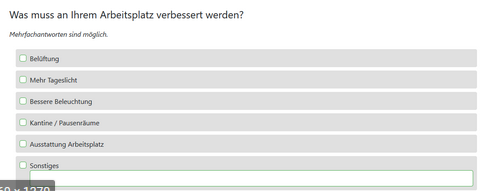
\includegraphics[width=0.8\textwidth]{pics/2ask_com.PNG}
    \centering
    \caption{Multiple-Choice-Frage von \cite{noauthor_fragebogen_nodate-2} }
    \label{fig:umfeld1}
\end{figure}

Von Interesse für designtechnische Aspekte ist die Angabe von sonstigen Antwortoptionen (siehe Abb. \ref{fig:umfeld1})
in Multiple-Choice-Fragen. Dieses Funktion deckt die Möglichkeit ab, dass keine der angegebenen Optionen für den 
Benutzer oder die Benutzerin in Frage kommt und optional eigene Antwortmöglichkeiten verwendet werden können. 
\newline
Ein tolles Feature für die Implementierung in die vorliegende Arbeit wäre die automatische Konvertierung 
sonstiger Optionen in vordefinierte Antwortmöglichkeiten. Umsetzen könnte man diese Konvertierung mittels algorithmischer Berechnungen.

\subsection{appinio.com}
Bei der Analyse dieses Tools stellte sich heraus, dass es sehr viele Funktionen beinhaltet. Die Auswertung liefert 
sehr ausführliche und mit vielen Details gespickte Informationen. Weiters ergab sich, dass das Tool für den Rahmen 
der Arbeit zu aufwendig gestaltet ist.

\begin{figure}[H]
    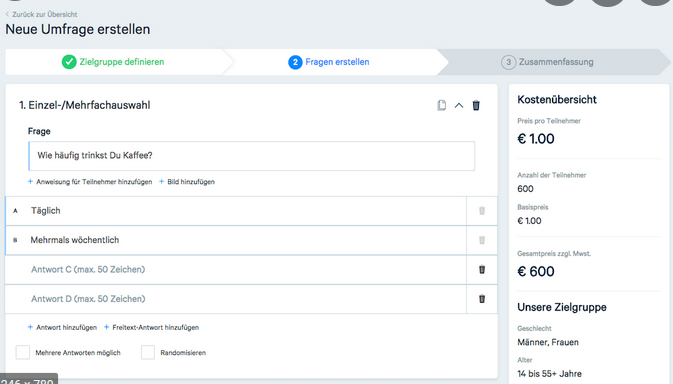
\includegraphics[width=0.8\textwidth]{pics/Appino_SteppsBeiErstellen.PNG}
    \centering
    \caption{Beispiel für die Erstellung eines Fragebogen von \cite{noauthor_fragebogen_nodate-3} }
    \label{fig:umfeld2}
\end{figure}

Das Design (siehe Abb. \ref{fig:umfeld2}) des Prozesses der Erstellung von Fragebogen ist sehr übersichtlich und optisch 
ansprechend umgesetzt. \cite{noauthor_fragebogen_nodate-3}

\subsection{ingress.com}
Das Tool Ingress deckt den Umfang der Arbeit mit seinen Funktionen ab. Mit ihm lassen sich Fragebögen erstellen, beantworten und auswerten. 
Während des Beantwortungsprozesses stellt Ingress ein Dashboard zur Verfügung, um den derzeitigen Stand der Umfrage zu überwachen.

\begin{figure}[H]
    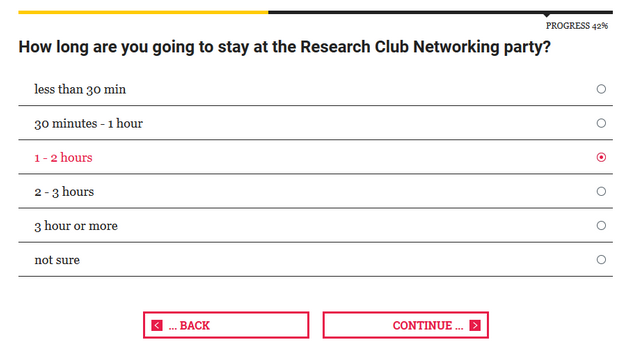
\includegraphics[width=0.8\textwidth]{pics/Ingress.PNG}
    \centering
    \caption{Fortschrittsanzeige bei der Beachtung der Fragebögen von \cite{noauthor_fragebogen_nodate-4} }
    \label{fig:umfeld3}
\end{figure}

Hervorzuheben bei diesem Tool ist die Fortschrittsanzeige, die während der Beantwortung von Umfragen (siehe Abb. \ref{fig:umfeld3}) angezeigt wird. 
Sie gibt den Benutzern eine direkte Rückmeldung über den Fortschritt und den Restaufwand, der betrieben werden muss, um 
das Ausfüllen des Fragebogens zu beenden. \cite{noauthor_fragebogen_nodate-4}

\subsection{questionpro.com}
Dieses Tool zeichnet sich durch das Analysieren der Daten in Echtzeit, die große Auswahl an Auswertungsdiagrammen und die 
resultierende genaue Auswertung aus. 

\begin{figure}[H]
    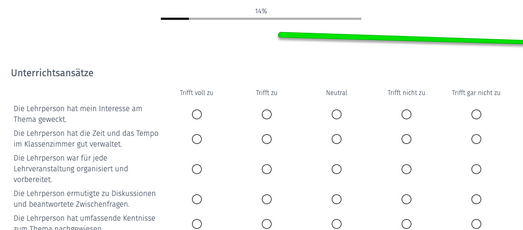
\includegraphics[width=0.8\textwidth]{pics/QuestionPro_Fortschrittsanzeige.PNG}
    \centering
    \caption{Fortschrittsanzeige bei der Beachtung der Fragebögen und Antwortoptionendesign von \cite{noauthor_fragebogen_nodate-5} }
    \label{fig:umfeld4}
\end{figure}

Dieses Tool bietet eine Fortschrittsanzeige, um Benutzerinnen und Benutzern eine direkte Rückmeldung über ihren derzeitigen Fortschritt zu geben.
(siehe Abb. \ref{fig:umfeld4}). Designtechnisch ist das Layout der Antwortoptionen von Interesse, da Optionen anders als 
Vergleichsobjekte nebeneinander statt untereinander angezeigt werden. Die Möglichkeit, diese Optionen nebeneinander 
anzuzeigen, ist nur dann sinnvoll, wenn die Optionen für jede Frage unverändert bleiben. Sollte das nicht der Fall sein, 
kann dadurch die Übersicht verloren gehen, da über jeder Antwortmöglichkeit ein anderer Text steht. \cite{noauthor_fragebogen_nodate-5}

\subsection{survio.com}
Bei diesem Tool war besonders das Herunterladen der Ergebnisse der Umfragen in vielen Formaten, beispielweise: PDF, DOCX, 
XLSX, CSV einprägsam.
\newline
\newline
Designtechnisch wurde auf die Verwendung von Radiobuttons verzichtet und stattdessen eine 
Auswahloption verwendet. Diese Option bietet dieselbe Funktionalität wie Radiobuttons, der / die Benutzer/in erkennt jedoch nicht 
auf den ersten Blick, welche Antwortmöglichkeiten die Frage hat. \cite{noauthor_fragebogen_nodate-6}

\subsection{umfrageonline.com}
Dieses Tool wurde genauer unter die Lupe genommen und es folgen die Erkenntnisse, die über das Design und die Funktionalitäten 
geschlossen wurden.

\begin{figure}[H]
    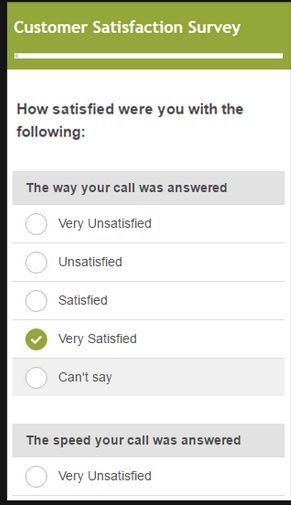
\includegraphics[width=0.3\textwidth]{pics/umfrageonline_com2.PNG}
    \centering
    \caption{Visuelle Trennung der Fragen von den Antwortoptionen von \cite{noauthor_fragebogen_nodate-7} }
    \label{fig:umfeld5}
\end{figure}

Das Tool zeigt (siehe Abb. \ref{fig:umfeld5}) eine visuelle Abtrennung von Fragen und Antwortmöglichkeiten, 
die hilft, nicht den Überblick bei einer großen Anzahl an Fragen und Antwortmöglichkeiten zu verlieren. 
Zudem dient es dazu, den Blick des Benutzers auf die Fragen zu fokussieren.
\begin{figure}[H]
    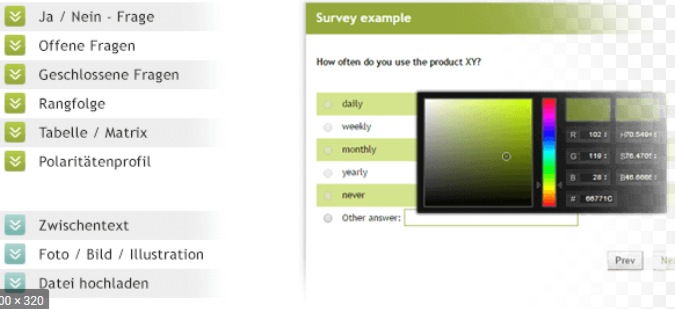
\includegraphics[width=0.8\textwidth]{pics/umfrageonline_com_erstellen.PNG}
    \centering
    \caption{Anpassung und Dateien zu einer Frage von \cite{noauthor_fragebogen_nodate-7} }
    \label{fig:umfeld6}
\end{figure}

Bilder oder Dateien, die zum Beantworten einer Frage nötig sind, zu einer Frage abzuspeichern, ist 
eine Funktionalität, die ein Fragebogentool von einem Anderen unterscheiden und abheben kann. Zudem ist die Funktion praktisch,
um wichtige Informationen zur Frage bereitzustellen. (siehe Abb. \ref{fig:umfeld6} als Beispiel). 
Den Umfang der Arbeit betrachtend, ist die in der Abbildung gezeigte Anpassung von Farben zu jedem Fragebogen zu aufwendig. 
Weiters wurden die Fragetypen analysiert. Die Implementierung aller Typen würde 
den Umfang der Arbeit überschreiten.

\begin{figure}[H]
    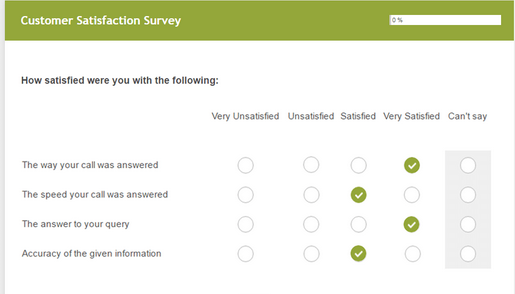
\includegraphics[width=0.8\textwidth]{pics/Umfrageonline_com_BlockanFragen.PNG}
    \centering
    \caption{Antwortoptionendesign von \cite{noauthor_fragebogen_nodate-7} }
    \label{fig:umfeld7}
\end{figure}

Dieses Tool bietet die Möglichkeit Antwortoptionen nebeneinander darzustellen.(siehe Abb. \ref{fig:umfeld7}). \cite{noauthor_fragebogen_nodate-7}, \cite{noauthor_pdflatex_nodate}

\begin{spacing}{1}
\chapter{Problembeschreibung}
\end{spacing}
\author{Weissengruber Nina}
Bei bereits existierenden Plattformen ist nicht sichergestellt, was mit den jeweiligen Daten passiert. 
Die Frage besteht darin, was mit den Daten geschieht, wie sie verwaltet werden oder ob sie an Dritte 
weiter gegegeben werden. Außerdem ist die Anonymität nicht sicher gestellt, 
da unsicher ist, ob irgendwelche persönlichen Daten zu den Personen, die die Umfrage durchführen, gesammelt oder 
an andere weitergeleitet werden.


\begin{spacing}{1}
\chapter{Aufgabenstellung}
\end{spacing}
\author{Weissengruber Nina}
Die Aufgabenstellungm der vorliegenden Arbeit, ist das Erstellen einer Fragebogen Plattform, 
bei der sichergestellt wird, dass die erhobenen Daten unter der Kontrolle des Fragenstellers bleiben, um so sämtliche datenschutzrechtlichen Aspekte zu erfüllen

In folgender Abbildung sieht man das Use-Case Diagramm für unsere Arbeit.

\begin{figure}[!htb]
    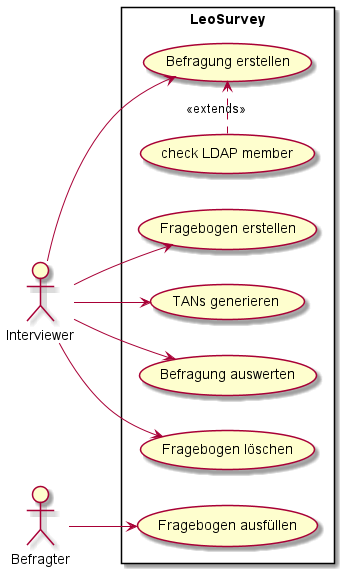
\includegraphics[width=0.5\textwidth]{pics/ucd.png}
    \centering
    \caption{Use Case Diagramm}
\end{figure}

Zunächst ist ein Fragebogen mit seinen Fragen zu erstellen. 
Anschließend wird eine Umfrage geplant (Bezeichnung der Umfrage, ev. Zeitraum der Umfrage, 
Teilnehmer der Umfrage). Danach werden Transaktionscodes (TAN) erstellt, 
um den Befragten eine anonyme Teilnahme an der Umfrage zu ermöglichen. Schließlich werden diese 
TANS an die Befragten übermittelt, woraufhin diese die Fragen des Fragebogens beantworten.


\begin{spacing}{1}
\chapter{Ziele}
\end{spacing}
\author{Weissengruber Nina}
Das Ziel dieser Diplomarbeit ist es, Personen eine simple und schnelle Möglichkeit zu bieten, um Umfragen zu erstellen. 
Dabei kann die Beantwortung der Fragen anonym ablaufen. Im Nachhinein sind die Daten leicht und 
schnell auswertbar.


\begin{spacing}{1}
\chapter{Systemarchitektur}
\end{spacing}
\setauthor{Weissengruber Nina}
\begin{figure}[!htb]
    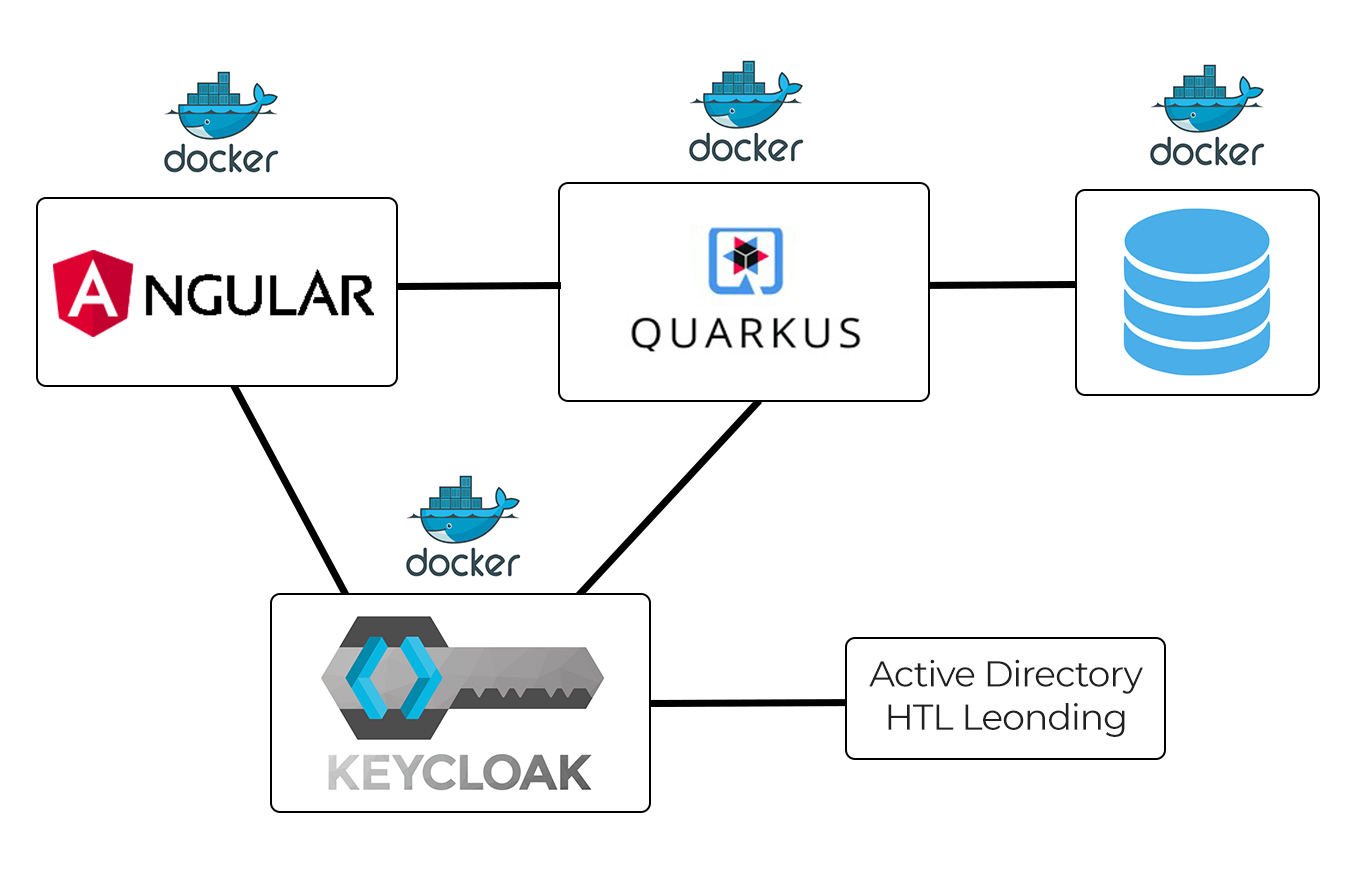
\includegraphics[width=0.5\textwidth]{pics/Systemarchitektur.png}
    \centering
    \caption{Systemarchitektur}
    \label{fig:systemarchitektur}
\end{figure}
In Abbildung \ref{fig:systemarchitektur} sieht man die Systemarchitektur.
Für diese Anwendung wurde für das Backend Quarkus verwendet, das auf eine PostgreSQL Datenbank zugreift.
Für das Frontend wurde Angular verwendet. Außerdem wurde ein Keycloak, der Zugriff auf das Active 
Directory der HTL Leonding hat und mit Frontend und Backend kommuniziert, eingebaut.

\section{Aktivitätsdiagramm}
Ein Aktivitätsdiagramm stellt eine Reihe von dynamischen Beziehungen in einem System dar.

\begin{figure}[!htb]
    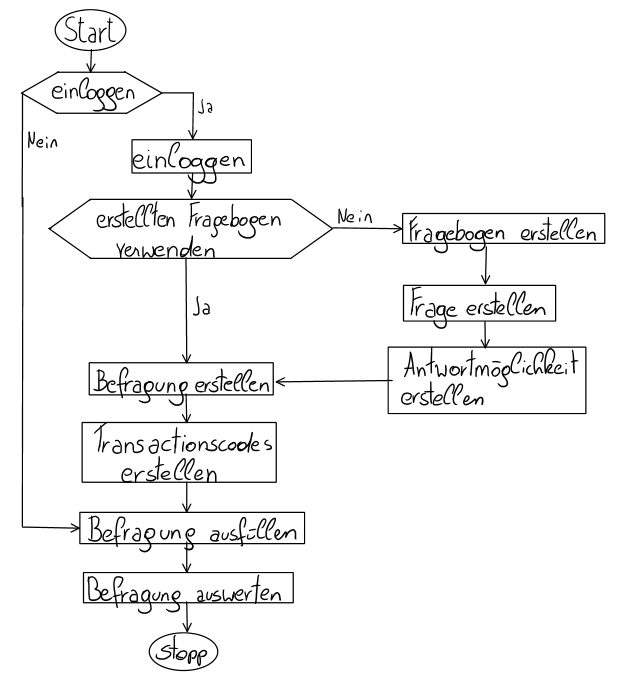
\includegraphics[width=0.5\textwidth]{pics/flussdiagramm.png}
    \centering
    \caption{Aktivitätsdiagramm}
    \label{fig:aktivitaetsdiagramm}
\end{figure}
Abbildung \ref{fig:aktivitaetsdiagramm}ist das Aktivitätsdiagramm für diese Arbeit.
Beim Start des Programms gibt es als erstes die Entscheidung, ob man sich einloggen will oder nicht. 
Möchte man sich nicht einloggen, kann man gleich die Befragung ausfüllen. Entscheidet man sich zum 
einloggen, steht man vor der Entscheidung, ob man einen bereits erstellten Fragebogen
verwenden möchte. Wenn ja, kann man eine Befragung erstellen. Möchte man keinen vorgefertigten Fragebogen 
verwenden, kann man selbst einen Fragebogen erstellen. Danach kann eine Frage erstellt und im Zuge 
dessen kann eine Antwortmöglichkeit/können Antwortmöglichkeiten erstellt werden. Danach ist es möglich, eine Befragung zu 
erstellen, um anschließend Transactions Codes zu erstellen. Danach kann man die Befragung 
ausfüllen und daraus die Befragung auswerten.

\setauthor{Raffeiner Christine}
\section{Klassendiagramm und Entity-Relationship-Modell}
\setauthor{Raffeiner Christine}
Beim Start der Arbeit wurden im Zuge der Implementierung 
ein Klassendiagramm und ein Entity-Relationship-Modell erstellt.

\subsection{Unterschied}
Bei beiden Diagrammtypen werden die Datenstrukturen und ihre Beziehungen zueinander abgebildet. 
Während jedoch Klassendiagramme dem objektorientierten Paradigma entsprechen (mit Collections, Objektidentität, usw.), 
bilden ERDs die in den Datenbanktabellen gespeicherten Datenstrukturen und deren Beziehungen ab. ERDs entsprechen dem 
relationalem Paradigma. (inkl. Erfüllung der Normalformen, des Schlüsselprinzips, usw.)
\newline
\newline
Die erste Version der Diagramme wurden mithilfe des SQL-Developers erstellt. Mehr Informationen zum SQL-Developer 
befinden sich im Kapitel \ref{chap:sqldeveloper}. \cite{noauthor_was_nodate-2}, \cite{noauthor_klassendiagramm_2022}, \cite{noauthor_klassendiagramm_nodate}

\subsection{Erste Version}
\begin{figure}[H]
    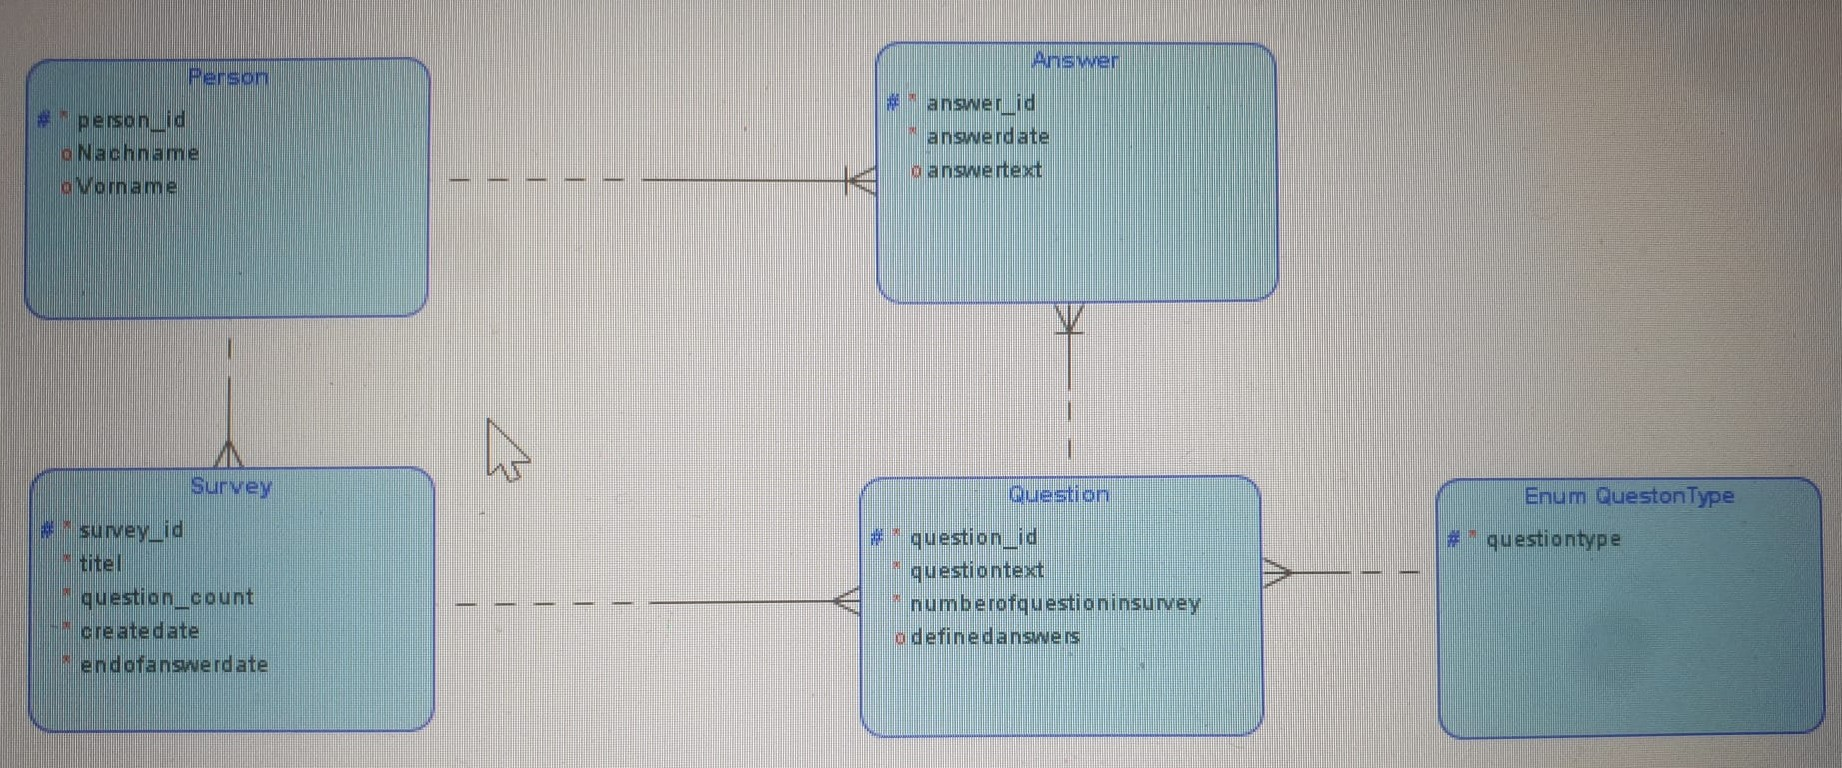
\includegraphics[width=0.8\textwidth]{pics/Datamodel_Version1.jpeg}
    \centering
    \caption{Erste Version des Datenmodelles (ERD)}
    \label{fig:cld1}
\end{figure}

\begin{figure}[H]
    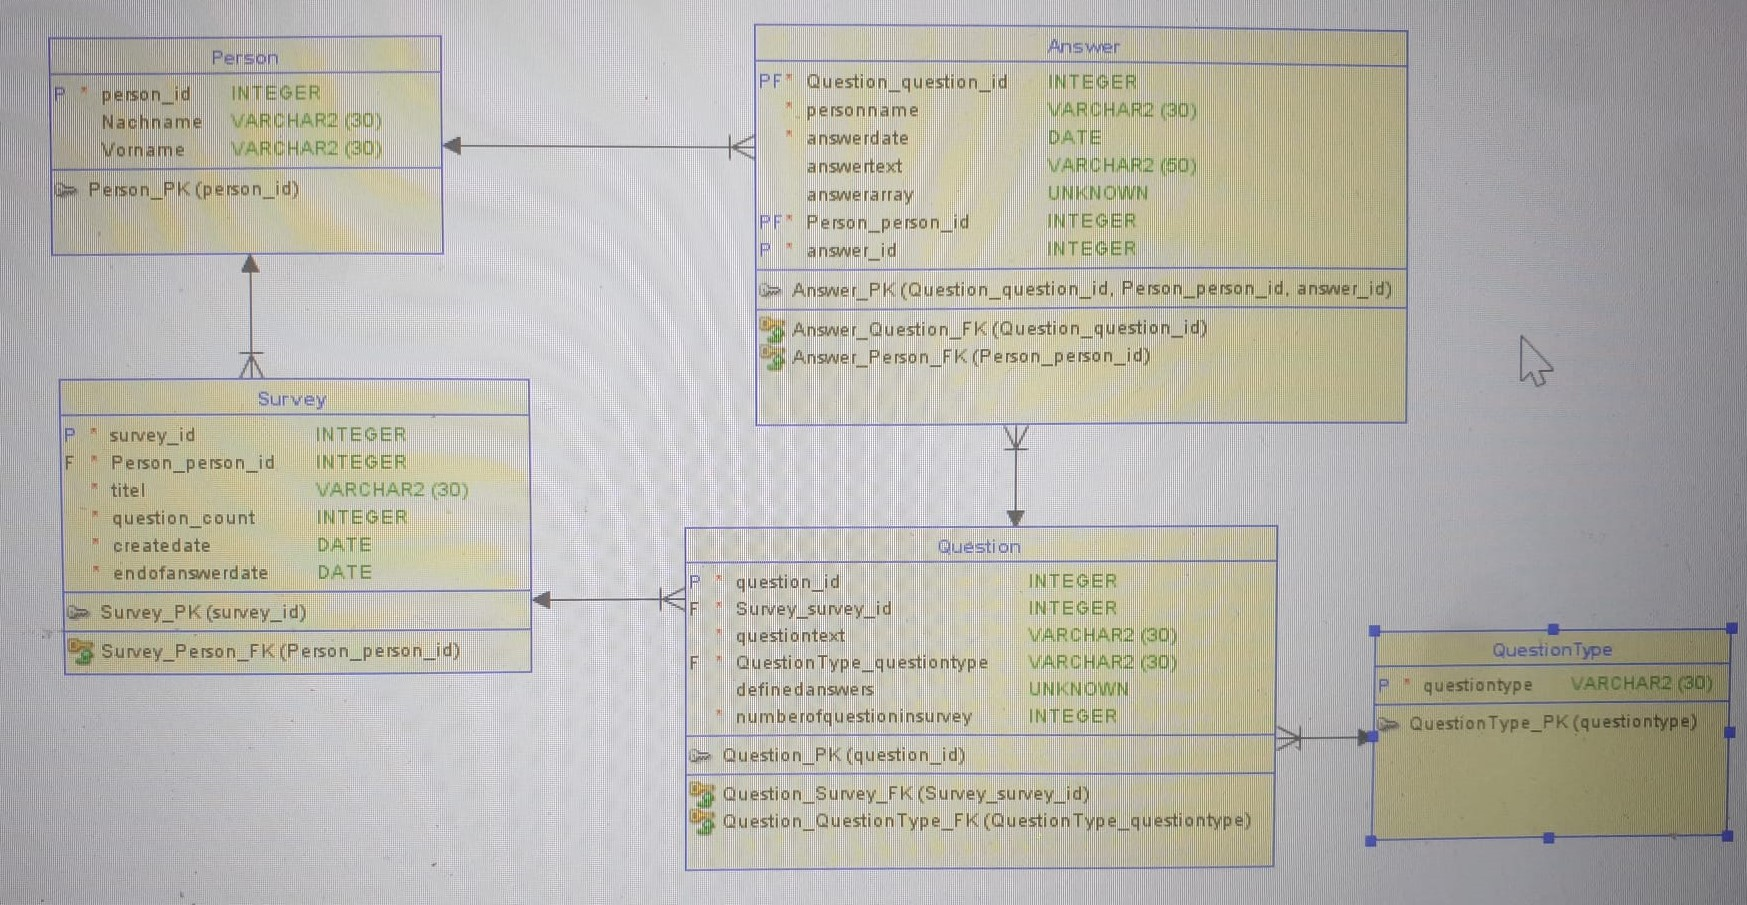
\includegraphics[width=0.8\textwidth]{pics/Datamodel_Vesion1_relational.jpeg}
    \centering
    \caption{Erste Version des Datenmodelles (CLD)}
    \label{fig:cld2}
\end{figure}
Das Datenmodell (siehe Abb. \ref{fig:cld1} und \ref{fig:cld2}) bildet eine einfache Art Fragebögen, 
zugehörige Befragungen und Antworten zu speichern, ab.
Für die leichtere Implementierung der grundlegenden Funktionen wurde in der ersten Version die Klasse Person noch zur 
Implementierung vorgesehen. Diese sollte in einer Endversion jedoch entfernt und durch die Anbindung an den Keycloak ersetzt werden.
\newline
\newline
Das Problem dieses Datenmodells bestand darin, dass nicht alle Anforderungen 
der Arbeit durch das Datenmodell abgebildet werden konnten und es auch nicht normalisiert wurde. 
\newline
Die erste Normalform wurde in dem Modell (siehe Abb. \ref{fig:cld1} und \ref{fig:cld2}) durch das Attribut definedanswers 
missachtet. Es war vorgesehen, alle möglichen Antworten in einem Attribut durch Trennzeichen abgetrennt zu speichern.
\newline
Es wurde dagegen entschieden, das Datenmodell zu überarbeiten und stattdessen ein neues Datenmodell von einem anderen Projekt als Vorlage 
zu nehmen. (siehe Kapitel \ref{chap:related_work}). 

\subsection{Normalisierung}
Unter Datenbanknormalisierung versteht man den Vorgang, Daten innerhalb einer Datenbank so effizient wie möglich zu organisieren.
Bei der Verwendung einer relationalen Datenbank kann die Normalisierung dazu beitragen, 
die Daten fehlerfrei zu halten und sicherzustellen, dass die Größe der Datenbank nicht durch 
doppelte Daten vergrößert wird. \cite{noauthor_normalisierung_2022}

\subsubsection{1. Normalform}
Die Erste Normalform (1NF) ist dann gegeben, wenn alle Informationen in einer Tabelle atomar vorliegen. \cite{noauthor_erste_nodate}

\subsection{Umstieg zu Markdown und PlantUML}
Alle weiteren Versionen des Datenmodells wurden mit PlantUML erstellt. Der Hauptgrund für den 
Wechsel bestand darin, dass die Software IntelliJ IDEA, die zum Programmieren des 
Backends verwendet wurde, diese Diagramme erstellen und anzeigen kann.
Diese können in Markdown eingebettet oder in eigenständigen Dateien mit einem Plugin gebildet werden. 
Die Teammitglieder waren mit PlantUML vertraut, was den Wechsel zusätzlich bestärkte.
\newline
\newline
Dateien mit Markdown-formatiertem Text können mit vielen Anwendungen geöffnet werden. 
Markdown-Dateien können einfach in andere Markdown-Anwendungen importieren werden.
Mehr Informationen über Markdown und PlantUML befinden sich im Kapitel \ref{chap:plantuml} und \ref{chap:markdown}.

\subsection{Zweite Version}
\begin{figure}[H]
    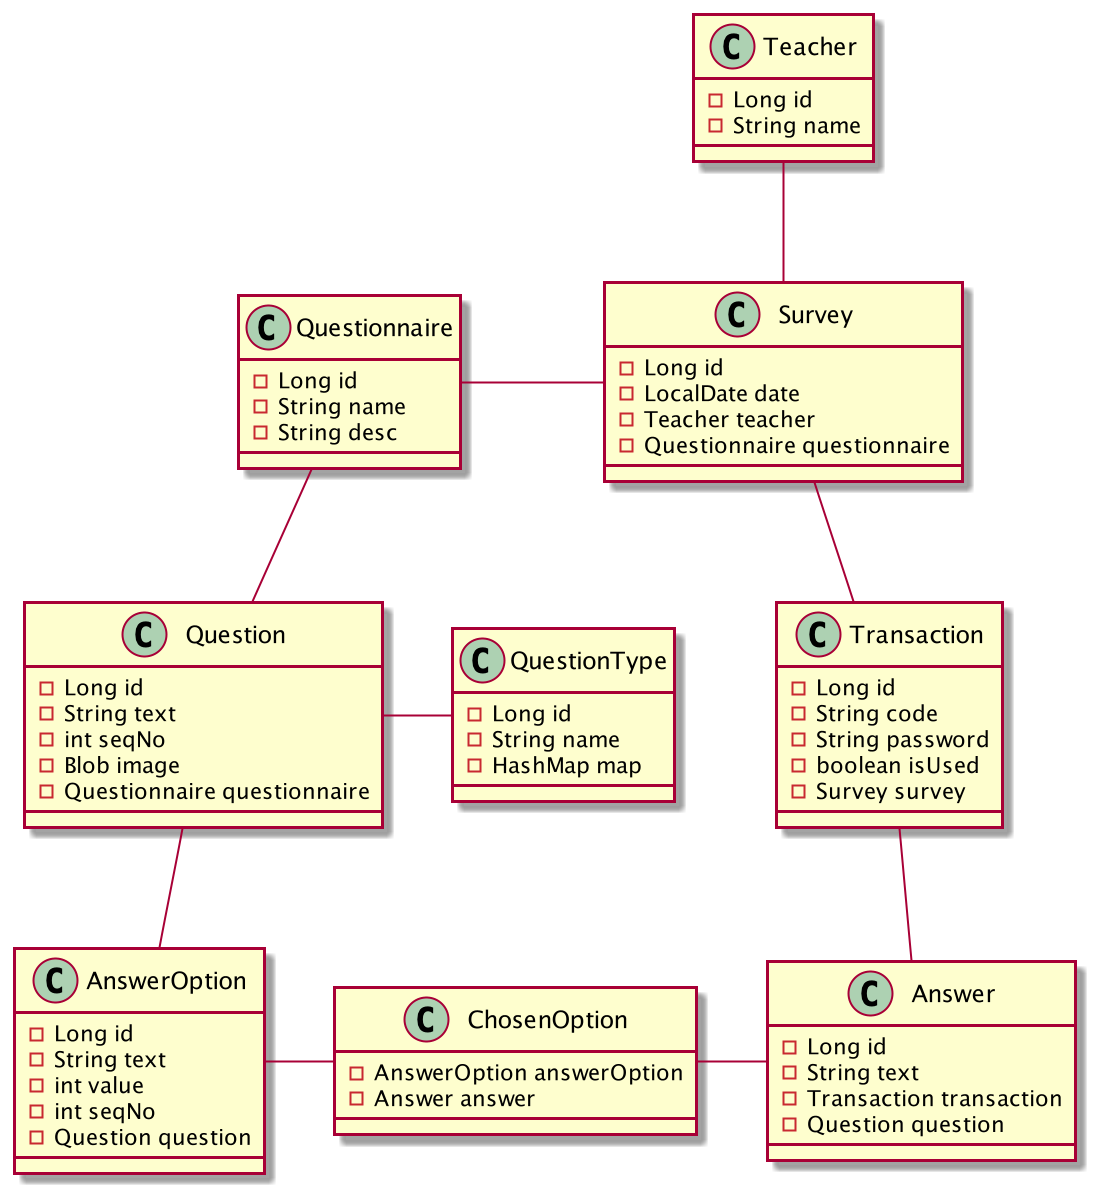
\includegraphics[width=0.8\textwidth]{pics/Datenmodel_Version2.png}
    \centering
    \caption{Zweite Version des Datenmodells}
    \label{fig:cld3}
\end{figure}
Die zweite Version des Datenmodells (siehe Abb. \ref{fig:cld3}) ist auf dem Modell eines Vorgängerprojektes aufgebaut 
(siehe Kapitel \ref{chap:related_work}). 
Erweiterungen wurden im Bereich Beantwortung der Befragung und Auswertung getätigt.
Mit den Erweiterungen konnten nun Singe-Choice, Multiple-Choice und Text-Antworten besser abgebildet werden.
Zudem wurde das Modell um die Funktion der optionalen Speicherung eines Bildes zu Fragen ergänzt.
\newline
\newline
Questionnaire stellt den Fragebogen und Survey die Befragungen dar. Es ergibt sich, dass für einen 
Fragebogen mehrere Befragungen gleichzeitig erstellt werden können.
Die Transaktionscodes stehen stellvertretend für den/die Benutzer/in und garantieren die Anonymität der Person, die den 
Fragebogen ausfüllt.

\subsection{Stabile Version}
\begin{figure}[H]
    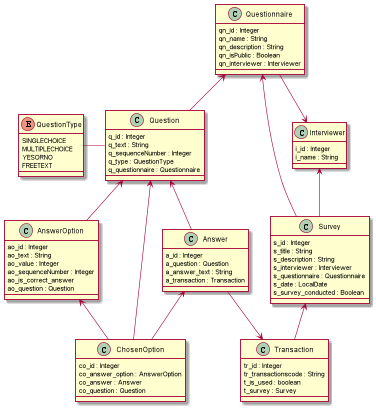
\includegraphics[width=0.8\textwidth]{pics/cld_Version3.png}
    \centering
    \caption{Zwischenversion des Datenmodells}
    \label{fig:cld4}
\end{figure}

Im Laufe der Implementierung sind weitere Änderungen am Klassendiagramm vorgenommen worden (siehe Abb. \ref{fig:cld4}), um den 
wachsenden Anforderungen gerecht zu werden. Dadurch ist beispielsweise ein zusätzliches 
Attribut im Fragebogen hinzugefügt worden (is\_public). Dieses Attribut stellt sicher, dass jede/r Benutzer/in der Applikation 
Fragebögen öffentlich zur Verfügung stellen kann. Sichtbar sind alle öffentlichen und privaten Fragebögen des Benutzers. 
\newline
Der Befragung wurde um das Attribut interviewer erweitert, um anderen Benutzern die Möglichkeit zu 
geben, öffentliche Fragebögen auszufüllen.
In der letzten signifikanten Änderung wurde das Attribut survey\_conducted hinzugefügt, 
dass besagt, ob und wie lange Personen den Fragebogen ausfüllen können. Dies dient 
dazu, den Fragebogen als Leistungsfeststellung zu verwenden.

\subsection{Endversion}
\begin{figure}[H]
    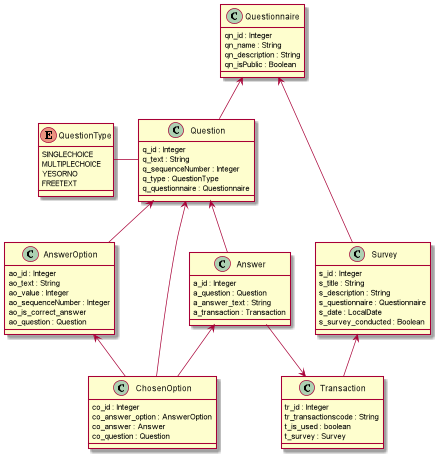
\includegraphics[width=0.8\textwidth]{pics/cld_final.png}
    \centering
    \caption{Letzte Version des Datenmodells}
    \label{fig:cld5}
\end{figure}

Mit der Implementierung des Keycloaks entfiel die Klasse Person. 
Die Speicherung der Nutzer/innen wurde durch den Keycloak übernommen. (siehe Abb. \ref{fig:cld5})


\begin{spacing}{1}
\chapter{Technologien}\label{chapter:tech}
\end{spacing}
\section{Angular}
\setauthor{Raffeiner Christine}
\begin{wrapfigure}{r}{0.3\textwidth}
    \begin{center}
      
\includegraphics[width=0.4\textwidth]{pics/Angular_Logo.png}
      \caption{Angular Logo von https://angular.io}
    \end{center}
\end{wrapfigure}
Angular ist ein TypeScript-basiertes, clientseitiges Webapplikations- und JavaScript-Framework 
was bedeutet, dass es für die Entwicklung von Webseiten und Webapplikationen ausgelegt ist. 
Es unterstützt die Verwendung des MVC(Model-View-Controller)-Pattern und vereinfacht die 
Erstellung und das Layoutieren von Single-Page-Applications (SPA) mit TypeScript,
HTML und einer Formatierungssprache. Mögliche Formatierungssprache sind CSS, SCSS SASS und Less.
\newline
\newline
Angular unterscheidet im Prinzip zwischen zwei Arten von Modulen. Zum Einen, das App-Modul, welches das Root-Module beinhaltet und als erstes Modul der Anwendung geladen und initialisiert 
wird und zum Anderen weitere Feature-Module, die sogenannten Components, Services und andere 
notwendige Dateien, die für ein bestimmtes Feature relevant sind.
Durch den Gebrauch des Model-View-Controller-Pattern von Angular wird die Wiederholung 
von Code mithilfe der Erstellung und Wiederverwendbarkeit von Komponenten, die 
statische HTML-Tags mit dynamischen Inhalten verbinden, verhindert.
\newline
\newline
Ein großer Vorteil von Angular ist es, dass es im Gegensatz zu anderen Frameworks über die Funktion 
einer bidirektionalen Verbindung verfügt. Das heißt, dass die Änderung eines 
Wertes einer Variable in einem Textfeld im HTML ebenfalls Auswirkungen auf die Variable im TypeScript 
hat und vice versa. Weitere Vorteile von Angular sind unter anderem, dass Angular ein 
Open Source Framework mit einer MIT Lizenz ist.
\newline
Weiteres stellt Angular umfangreiche Funktionen zur Verfügung, die direkt bereitgestellt sind.
Wie diese Funktionen zu implementieren sind, wird von Angular bereits vorgegeben und erspart somit 
die Überlegung der Implementierung. Zudem werden Zeit und fallweise Kosten gespart, da diese nicht erst
selbst programmiert werden müssen. \cite{noauthor_angular_nodate}, \cite{noauthor_angular_2021}

\subsection{TypeScript}
\begin{wrapfigure}{r}{0.3\textwidth}
    \begin{center}
      
\includegraphics[width=0.4\textwidth]{pics/TS_Logo.png}
      \caption{TypeScript Logo von https://thenewstack.io/how-typescript-helps-enterprise-developers/}
    \end{center}
\end{wrapfigure} 
TypeScript ist eine Programmiersprache, die von Microsoft entwickelt und gewartet wird. 
Sie ist eine streng syntaktische Variante von JavaScript und fügt der Sprache eine optionale 
statische Typisierung hinzu. Es kann zur Entwicklung von JavaScript-Anwendungen sowohl für 
die clientseitige als auch für die serverseitige Ausführung verwendet werden. TypeScript ist für 
die Entwicklung großer Anwendungen konzipiert und lässt sich in JavaScript umwandeln. 
\newline
TypeScript ist keine Programmiersprache für sich allein. Es ist vielmehr eine Kombination aus Werkzeugen und 
optionalen, entfernbaren Typen. TypeScript ermöglicht es einem beliebige 
JavaScript-Tools, -Bibliotheken und -Frameworks zu verwenden.
\newline
TypeScript bezieht sich auf mehrere verschiedene Dinge:
\begin{itemize}
    \item einen Type-Checker für die beiden Sprachen TypeScript und JavaScript
    \item eine übergeordnete Sprache, die die Typensyntax zu JavaScript hinzufügt
    \item den offizielle Compiler, der Code typisiert und umwandelt
\end{itemize}
All diese Komponenten werden benötigt, um JavaScript eine statische Typisierung hinzuzufügen 
und Werkzeuge bereitzustellen, die die Verwendung einfach und komfortabel machen.
\newline
Der TypeScript-Compiler ist selbst in TypeScript geschrieben und zu JavaScript kompiliert. Er ist unter der Apache 
License 2.0 lizenziert. \cite{noauthor_typescript_2022}, \cite{noauthor_softwareentwicklung_nodate}

\subsubsection{JavaScript}
JavaScript (kurz JS) ist leichtgewichtige, interpretierte Skriptsprache. Ihre Bekanntheit hat 
sie hauptsächlich als Skriptsprache für Webseiten erhalten, um Benutzerinteraktionen auszuwerten, 
Inhalte zu verändern, nachzuladen oder zu generieren. JavaScript wird auch außerhalb von Browsern 
angewandt und dient ebenfalls für die Programmierung von Prototypen. Die Sprache bietet 
sowohl objektorientierte, aber klassenlose, imperative als auch deklarative Programmierung an. 
Der Standard für JavaScript ist ECMAScript. \cite{noauthor_javascript_nodate}, \cite{noauthor_javascript_2022}, \cite{noauthor_javascript-grundlagen_nodate}

\subsection{CSS}
\begin{wrapfigure}{r}{0.3\textwidth}
    \begin{center}
      
\includegraphics[width=0.2\textwidth]{pics/CSS_Logo.png}
      \caption{CSS Logo}
    \end{center}
\end{wrapfigure} 
CSS auch Cascading Style Sheets ist eine Formatierungssprache für HTML-, SVG- und XML-Dokumente.
Somit behandelt CSS das Design oder den Stil und nicht den Inhalt von Webseiten. 
Beispielsweise können damit Schriftarten, Farben, Linien, Höhen, Breiten und Positionierung auf einer 
Webseite definieren werden. CSS ermöglicht es ein einmal erstelltes Design schnell und 
einfach in ein anderes Projekt zu übertragen. CSS stellt einen Standard dar und wird vom 
World Wide Web Consortium (W3C) gemanagt und weiterentwickelt. 
\newline
Darüber hinaus wird eine responsive Darstellung von CSS unterstützt. Anders gesagt heißt dass, das mittels CSS 
passende Darstellungsformen für unterschiedliche Geräte angefangen von Monitoren zu Druckern 
bis hin zu Smartphones definiert werden können. Mittels Media Queries können in CSS auch Geräteeigenschaften Breite und Höhe des Browserfensters
ausgelesen werden. Eigenschaften, die bestimmt werden können sind:
\begin{itemize}
    \item Breite und Höhe des Gerätes
    \item Orientierung (Quer- oder Hochformat)
    \item Bildschirmauflösung
\end{itemize}
CSS wird von allen gängigen Browsern 
unterstützt, allerdings kann es zu Einschränkungen bzw. Fehlern bei der Darstellung des Layouts in 
Browsern kommen - übermäßig davon betroffen sind veraltete Browser. \cite{noauthor_css_nodate}, \cite{noauthor_cascading_2022}, \cite{noauthor_css_nodate-1}, \cite{noauthor_css_nodate-2}

\subsubsection{World Wide Web Consortium}
Beim World Wide Web Consortium (W3C) handelt es sich um ein Gremium, dass technische 
Spezifikationen und Richtlinien zur Standardisierung der Techniken im World Wide Web entwickelt.
Andere bekannte Beispiele für Technologien, die durch das W3C standardisierte werden sind, HTML 
SVG und XML. \cite{noauthor_world_nodate}, \cite{noauthor_world_2022}

\subsection{SCSS}
SCSS ist die erweiterte Version von CSS. Es können Variablen definiert werden, die zur Folge haben, dass
der Code verkürzt wird. \cite{noauthor_unterschied_nodate}

\subsection{SASS}
\label{chap:stylesheet}
SASS basiert auf Ruby und heißt ausgeschrieben SassScript. Es steht unter der MIT-Lizenz und gilt daher als Open Source.
SASS bietet im Gegensatz zu CSS zusätzlich die Funktion von: 
\begin{itemize}
    \item Variablen (wie SCSS)
    \item Mathematische Funktionen wie Multiplizieren, Dividieren, Addieren und Subtrahieren (+, -, *, / )
    \item Funktionen
    \item Schleifen
    \item Fallunterscheidungen (wie if und else)
    \item Mixins (Vorlagen, die selbst erstellt oder bei der Verwendung eines Frameworks einfach in den eigenen Code eingebettet werden können)
    \item Vererbung (mittels Selektor)
\end{itemize}
Ein großer Nachteil von SASS ist, dass es zuerst kompiliert werden muss. Das heißt anders als in CSS,
wo Änderungen in der CSS-Datei sofort Auswirkungen auf der Webseite haben, müssen in SASS die Änderungen
erst in CSS übersetzt werden. Im Gegensatz dazu spricht für SASS die freie Auswahl der Syntax. Ob man nun die vorgegebene 
Syntax benutzt oder lieber die gewohnte SCSS- / CSS-Syntax verwendet. \cite{noauthor_sass_nodate}, \cite{noauthor_sass_nodate-2}, \cite{noauthor_grose_nodate}

\subsection{Less}
Genau wie SCSS oder SASS ist Less eine Obermenge von CSS- und somit ebenfalls eine Stylesheet-Sprache.
Vergleichsweise zu SASS ist die Verwendung von Mixins (Vorlagen), Variablen, Berechnungen und Verzweigungen.
Less ist in JavaScript geschrieben und muss ebenfalls kompiliert werden. Allerdings können 
Mithilfe eines Watch-Mode Änderungen automatisch im Webbrowser angezeigt werden. \cite{noauthor_sass_nodate-1}, \cite{noauthor_less_nodate}

\subsection{HTML}
\begin{wrapfigure}{r}{0.3\textwidth}
  \begin{center}
    
\includegraphics[width=0.2\textwidth]{pics/HTML_Logo.png}
    \caption{CSS Logo von https://de.wikipedia.org/wiki/HTML5}
  \end{center}
\end{wrapfigure} 
HTML - ausgeschrieben Hypertext Markup Language - ist eine bekannte textbasierte Auszeichnungssprache für die 
Anzeige und Strukturierung von Webseiten. HTML macht sich sogenannte Tags zu Nutze, um die verschiedensten
Inhalte wie Text, Bilder oder Videos anzuzeigen. Der derzeitige Standard von HTML ist XHTML (Extensible Hypertext Markup Language) und HTML5.
XHTML gehört zu XML, einer Auszeichnungssprache und Dateiformat und erweitert die Auszeichnungssprache HTML.
\newline
HTML5 enthält detaillierte Verarbeitungsmodelle, um mehr kompatible Implementierungen zu fördern: 
Es erweitert, verbessert und vereinfacht das für Dokumente verfügbare Format und führt 
Formatierungs- und Anwendungsprogrammierschnittstellen (APIs) für komplexe Webanwendungen ein. HTML5 ist 
vermehrt für Suchmaschinen optimiert und fördert im Gegensatz zu alten Versionen userorientierte Webseiten.
Zusätzlich zu den Anzeigeelementen verfügt HTML über nicht sichtbare Inhalte namens Metadaten. Diese Daten sind im normalen 
Gebrauch und für User nicht sichtbar. Suchmaschinen allerdings können sie lesen und nicht nur das, sondern auch ihre Suchergebnisse dahingehend
anpassen. Befinden sich keine Metadaten im HTML-Code, versuchen Suchmaschinen sich etwas von der Webseite zusammenzulesen.
HTML-Quellcode kann in jedem Editor geschrieben und von jedem Browser interpretiert werden. \cite{noauthor_hypertext_2022}, \cite{noauthor_html_nodate}, \cite{noauthor_html_nodate-1}

\subsection{NodeJS}
\begin{wrapfigure}{r}{0.3\textwidth}
  \begin{center}
    
\includegraphics[width=0.2\textwidth]{pics/NodeJS_Logo.png}
    \caption{NodeJS Logo von https://de.wikipedia.org/wiki/HTML5}
  \end{center}
\end{wrapfigure}
Node.js ist ein plattformübergreifendes Open-Source Framework, die der MIT-Lizenz unterliegt, und für 
die Entwicklung eigenständiger JavaScript-Programme, Netzwerktools und Webapplikationen verwendet wird.
Der JavaScript-Code kann außerhalb von Webbrowsern laufen und bietet neben Netzwerk-orientierten 
Kommandozeilen-Tools auch Werkzeuge für die Systemadministration. 
Node.js wird in Googles JavaScript-Laufzeitumgebung V8, einer prozessbasierten virtuellen Maschine 
ausgeführt, die den Code mithilfe eines Compilers in Maschinensprache übersetzt.  
\newline
\newline
Besonders für die Verwendung von Angular ist NodeJS von Bedeutung, da die geschriebene Applikation 
mit dem Node Package Manager, kurz npm mit beliebigen Modulen erweitert werden kann. Der Node Package Manager
kann dabei allerdings nicht nur Module samt ihrer Abhängigkeiten installieren, sondern diese ebenfalls
entfernen, kompilieren und auf neuere oder bestimmte Version aktualisieren. Diese Prozesse werden mithilfe
des Node.js-Repository zur Verfügung gestellt. \cite{nodejs_nodejs_nodate}, \cite{noauthor_nodejs_2022}, \cite{noauthor_nodejs_nodate}

\subsection{Angular Materials}
\label{chap:materials}
Die Angular Material UI ist eine Bibliothek, die es ermöglicht, verschiedene Komponenten zu importieren
und zu verwenden, um Benutzeroberflächen in Angular zu erstellen. Diese importieren Komponenten können gegebenfalls in einem vordefinierten 
Rahmen an die jeweiligen Anforderungen angepasst werden. Das heißt, dass in einer ausgewählten Komponente 
einzelne Teilbereiche zum Beispiele ausgeblendet (nicht verwendet) oder eingeblendet 
(verwendet und definiert) werden können. Die Verwendung von Materials spart einiges an Zeit, 
da man nicht alle Funktionen von Grund auf selbst programmieren muss. Zusätzlich zu den bereits implementierten
Funktionen liefert Angular Materials auch Layoutierungsregeln, Darstellungsregeln und Animationen (vordefiniertes CSS beziehungsweise JavaScript).
Diese Regeln können voneinander abweichen je nachdem welches Theme gewählt wird.
\newline
\newline
Themes definieren einen Satz klar definierter Darstellungsregeln. Beispielsweise wird der Hintergrund von ein und demselben Element
mit unterschiedlichen Themes verschieden eingefärbt. Ein klassisches Beispiel hierfür sind der Helle und Dunkle Modus
von vielen Webseiten und Programmen. Es ist allerdings auch möglich eigene Themes festzulegen.
All diese Aspekte machen das Erstellen visuell ansprechender und funktional 
userfreundlicher Anwendungen um einiges leichter. \cite{noauthor_angular_nodate-1}, \cite{noauthor_official_2022}

Beispiele für die in Angular Materials verwendeten Komponenten:
\begin{itemize}
  \item Toolbar
  \item Checkbox
  \item Expansion Panel
  \item Form field
  \item Stepper
  \item Pageinator
  \item Radio button
  \item Tabs
  \item etc. \cite{noauthor_name_nodate}
\end{itemize}

\subsection{angular-oauth2-oidc}
Das Modul angular-oauth2-oidc wird für die Kommunikation mit dem Keycloak verwendet. Es bietet 
mehrere Funktionen, die die Kommunikation vereinfachen und erleichtern. \cite{noauthor_angular-oauth2-oidc_nodate}
\begin{itemize}
  \item Lauffähig mit allen modernen Browsern und IE
  \item Automatisches Aktualisieren eines Tokens, wenn/einige Zeit bevor es abläuft
  \item Konfigurierbare Anmelde- und Abmelde-Funktion
\end{itemize}

\subsubsection{Anmerkungen zu den Features}
Die Lauffähigkeit für alle modernen Browser ist in der modernen Zeit eigentlich ein Muss, da der Benutzer die Freiheit
haben sollte, seinen präferierten Browser zu nutzen.
Das automatische Aktualisieren des Tokens, sollte dieser abgelaufen sein, verbessert die Userfreundlichkeit, 
da der Benutzer sich nicht neu einloggen muss oder anderweitig einen neuen Token anfordern muss.

\subsubsection{Logging out Funktion}
Die Logout-Methode löscht den zugewiesenen Token-Speicher (standardmäßig sessionStorage) und 
leitet den Benutzer an den Logout-Endpunkt des Auth-Servers weiter, falls ein solcher 
konfiguriert wurde.

\subsubsection{Logging in Funktion}
Die Funktion bietet die Möglichkeit den Benutzer an die angegebene URL des Identitäts-Anbieters weiterzuleiten.
Nach einer erfolgreichen Anmeldung wird der Benutzer zu einer in der Konfiguration angegebenen URL auf der Webseite umgeleitet.
Alternativ kann angegeben werden, dass die Anmeldung übersprungen wird.

\subsection{angular/localize}
Das Paket angular/localize enthält Hilfestellungen und Werkzeuge für die Lokalisierung einer Angular 
Anwendung. Die Idee dahinter besteht darin, dass Texte, die übersetzt werden sollen, mit 
speziellen Tags markiert werden. Die Übersetzung selbst kann einerseits entweder zur Laufzeit im Browser erfolgen oder
andererseits durch Markierungen im Code und einem statischen Nachbearbeitsungswerkzeug, der den Originaltext durch 
übersetzten Text ersetzt, bevor der Code bereitgestellt wird.
Für jede Sprache wird eine eigene Ausgangssprachdatei bereitgestellt, die Schlüssel-Wert-Paare mit Nachrichtenbezeichnern 
als Schlüssel und lokalisierten Nachrichten als Werte enthält.
Für das Format der Datei kann XLIFF 1.2 (Standart), XLIFF 2 oder in XML-Message Bundle (XMB) verwendet werden.
Die Ausgangssprachdatei muss als Identifikation der Sprache mit einem Sprachkürzel (ISO 639-2) versehen werden 
um die Sprache, das Land zu spezifizieren. 
\cite{noauthor_xml_2020}, \cite{noauthor_localization_nodate}, \cite{noauthor_angular_nodate-2}, \cite{noauthor_angular_nodate-3}, \cite{noauthor_angularlocalize_nodate}, \cite{noauthor_angular_nodate-4}

\subsubsection{Beispiele für Sprachkürzel}
\begin{itemize}
  \item en
  \item en\_Us
  \item fr
  \item de
\end{itemize}

\subsubsection{XLIFF 1.2 und XLIFF 2}
XLIFF (XML Localization Interchange File Format) ist ein XML-basiertes Bitext-Format, das zur 
Standardisierung der Übermittlung von Lokalisierungsdaten zwischen verschiedenen Tools während 
eines Lokalisierungsprozesses entwickelt wurde.
Im Vergleich zu XLIFF 1.2 hat XLIFF 2.0 eine anders organisierte DOM-Struktur und andere
Anwendung der Modularität. \cite{noauthor_xliff_2022}, \cite{noauthor_xliff-dateien_nodate}

\subsubsection{XML Message Bundle}
Der länderspezifische Text wurde in separate XML-Dateien extrahiert. 
Diese werden lose als XML-Ressourcenbündel bezeichnet und je nach Gebietsschema abgerufen und 
durchsucht. \cite{noauthor_xml_nodate}, \cite{noauthor_message_nodate}, \cite{noauthor_xml_nodate-1}

\section{Docker}
\setauthor{Raffeiner Christine}
\begin{figure}[H]
  
\includegraphics[width=0.2\textwidth]{pics/Docker_Logo.png}
  \centering
  \caption{CSS Logo von https://www.cloudflight.io/de/blog/docker-container-die-zukunft-moderner-applikationen-und-multi-cloud-deployments/}
\end{figure}
Docker ist eine Open-Source Softwareplattform für die Erstellung, Lieferung und Ausführung von Anwendungen. \cite{noauthor_home_nodate}
Docker teilt sich in die Bestandteile: 
\begin{itemize}
  \item Docker-Container
  \item Dockerfile
  \item Container-Images
  \item Docker run
  \item Docker Hub
  \item Docker Engine
  \item Docker Compose
  \item Docker Desktop.
\end{itemize}

\subsection{Docker Container}
Docker Container sind kleine und leichtgewichtige Ausführungsumgebungen, die den Kernel des 
Betriebssystems gemeinsam nutzen, ansonsten aber isoliert voneinander laufen und 
über ein eigenes Dateisystem verfügen. Durch die Perfektionierung dieses Prinzips hat Docker sich 
schnell zu einem De-facto-Industriestandard für Container entwickelt.
\newline
\newline
Docker-Container ermöglichen Kompositionsfähigkeit. Container erleichtern es den Entwicklern, die 
Bausteine einer Anwendung zu einer modularen Einheit mit leicht austauschbaren Teilen  
zusammenzustellen, was Entwicklungszyklen, Funktionsfreigaben und Fehlerbehebungen beschleunigen 
kann. Docker-Container sind zustandslos und unveränderlich. Container booten und laufen von einem Image, 
dass ihren Inhalt beschreibt. Dieses Image ist standardmäßig unveränderlich - einmal erstellt, 
ändert es sich nicht mehr. Eine Container-Instanz ist jedoch vergänglich. Wenn der Container aus dem 
Systemspeicher entfernt wird, ist er für immer verschwunden. \cite{noauthor_docker_nodate}, \cite{noauthor_install_nodate}, \cite{noauthor_docker_2022}, \cite{noauthor_was_nodate-5}

\subsubsection{Unterschied zu Virtuellen Maschinen}
Eine virtuelle Maschine (VM) ist die Virtualisierung / Emulation eines Computersystems. 
Virtuelle Maschinen bieten die Funktionalität eines physischen Computers. 
Sie sind isoliert vom Rechner, auf dem die virtuelle Maschinen laufen.
Jede VM benötigt ihr eigenes Betriebssystem, was bedeutet, dass sie in der Regel viel Speicherplatz benötigen und daher
langsam starten, schwierig zu bewegen und umständlich zu warten und zu aktualisieren sind. \cite{noauthor_virtuelle_2021}, \cite{noauthor_was_nodate-6}

\begin{figure}[H]
  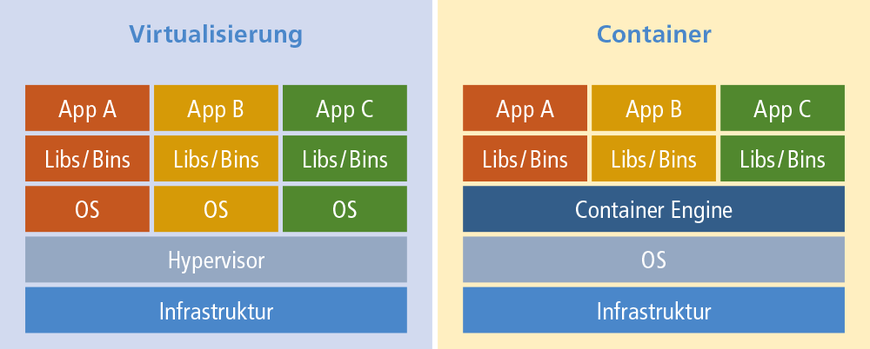
\includegraphics[width=0.8\textwidth]{pics/Container_VM.png}
  \centering
  \caption{Unterschied von Virtuellen Maschinen und Containern von https://www.shd-online.de/fachartikel/der-app-store-fuer-server-wofuer-sie-container-brauchen/}
\end{figure}

\subsection{Dockerfile}
Jeder Docker-Container beginnt mit einem Dockerfile. Diese Textdatei enthält eine 
Reihe von Anweisungen zur Erstellung eines Docker-Abbilds, einschließlich des Betriebssystems, 
der Sprachen, der Umgebungsvariablen, der Dateispeicherorte, der Netzwerk-Ports und aller anderen 
Komponenten, die zur Ausführung benötigt werden.

\begin{figure}[H]
  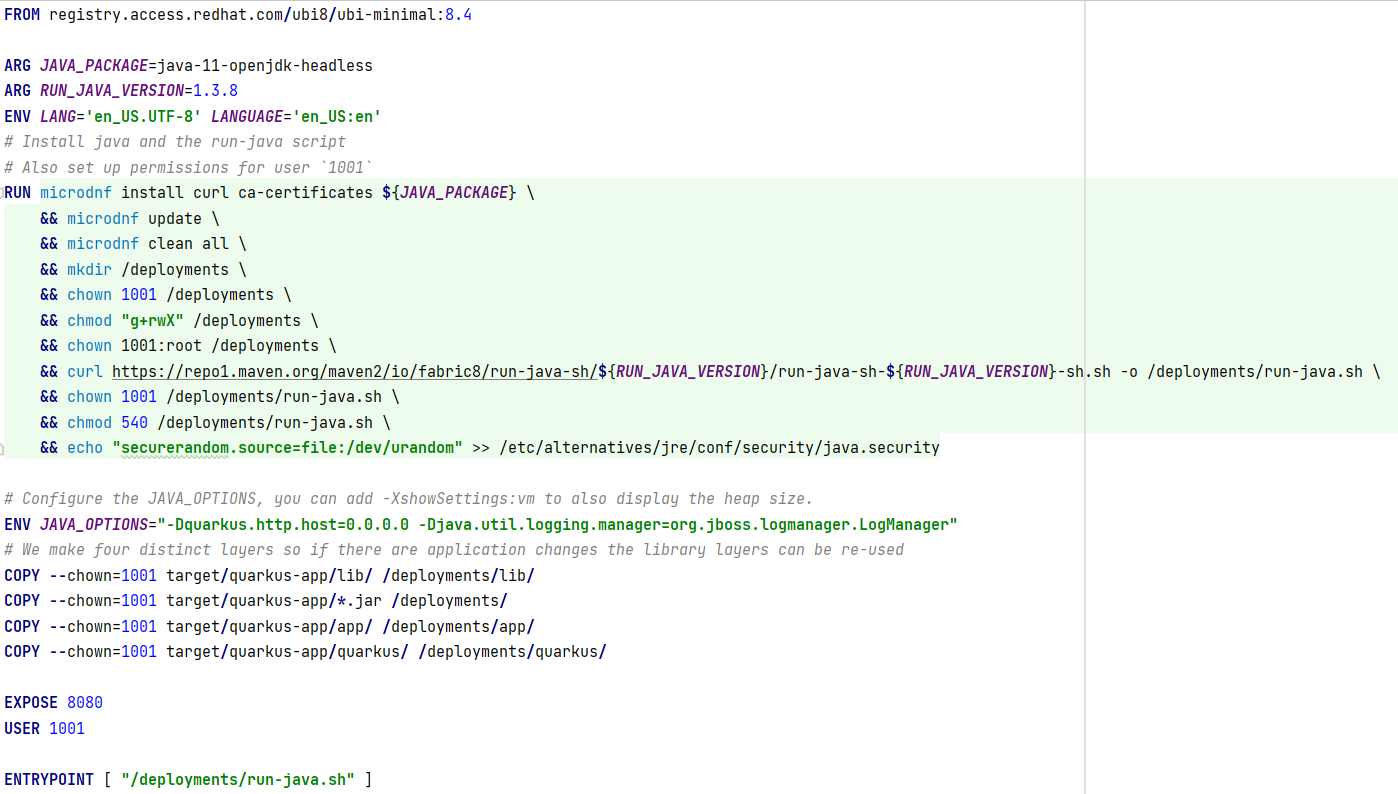
\includegraphics[width=0.8\textwidth]{pics/Bsp_Dockerfile.PNG}
  \centering
  \caption{Beispiel eines Dockerfiles}
\end{figure}

\subsection{Container-Images}
Ein Docker-Image ist eine andere Möglichkeit einen Docker-Container zu erstellen.
Ein Docker-Image ist eine portable, schreibgeschützte, ausführbare Datei, die die Anweisungen zur 
Erstellung eines Containers und die Spezifikationen dafür enthält, welche Softwarekomponenten der 
Container wie ausführen wird. Jeder Container ist eine Instanz eines Images, wobei mehrere Instanzen 
desselben Images gleichzeitig ausgeführt werden können. Diese Cluster von Containern müssen dann orchestriert werden, 
wozu in der Regel Kubernetes eingesetzt wird. \cite{noauthor_docker_nodate-2}

\subsubsection{Kubernetes}
Kubernetes ist eine flexible, erweiterbare Open-Source-Plattform für die Verwaltung von
containerisierten Systemen und Diensten, die sowohl eine deklarative Konfiguration als auch eine 
Automatisierung ermöglicht. \cite{noauthor_kubernetes_2021}, \cite{noauthor_was_nodate-7}

\begin{itemize}
  \item Automatisierte Terminplanung
  \item Automatisierte Rollouts und Rollbacks
  \item Horizontale Skalierung und Lastausgleich
  \item Bietet eine konsistente Umgebung für Entwicklung, Tests und Produktion
  \item Automatisch skalierbare Infrastruktur
\end{itemize}

\subsection{Docker run}
Docker run ist der Befehl von Docker, mit dem ein Container gestartet wird.
Es können Spezifikationen zum Beispiel für den Namen des Containers und den Port, auf dem der Container
laufen soll, getroffen werden.

\subsection{Docker Hub}
Docker Hub ist ein Repository, in dem Container-Images gespeichert, freigegeben und verwaltet werden 
können. Es ist mit den GitHub-Repository für GitHub zu vergleichen, nur werden im Docker Hub Images 
zur Verfügung gestellt. Startet man einen Container eines Images wird mit den Standardeinstellungen dieses 
Image automatisch auf Docker Hub gesucht und wenn gefunden, heruntergeladen. \cite{noauthor_docker_nodate-1}

\subsection{Docker-Engine}
Die Docker-Engine ist die zugrunde liegende Client-Server-Technologie, die 
Container erstellt und ausführt. Die Docker-Engine umfasst einen 
langlaufenden Daemon-Prozess zur Verwaltung von Containern, APIs, die es 
Programmen ermöglicht, mit dem Docker-Daemon zu kommunizieren, sowie eine 
Befehlszeilenschnittstelle bildet.

\subsection{Docker Compose}
Docker Compose ist ein Tool, das YAML-Dateien verwendet, um Multicontainer-Docker-Anwendungen 
zu definieren und auszuführen. Es ermöglicht Ihnen, alle Dienste Ihrer Konfiguration zu erstellen, 
zu starten, zu stoppen und neu zu erstellen und den Status und die Protokollausgabe 
aller laufenden Dienste anzuzeigen.

\subsubsection{YAML}
YAML ist eine für Sprache zur Daten-Serialisierung. Sie wird üblicherweise für Konfigurationsdateien 
und in Anwendungen verwendet, in denen Daten gespeichert oder übertragen werden. YAML verwendet Schlüssel-Wert-Paaren. \cite{noauthor_yaml_2022}, \cite{noauthor_einfuhrung_2021}

\begin{figure}[H]
  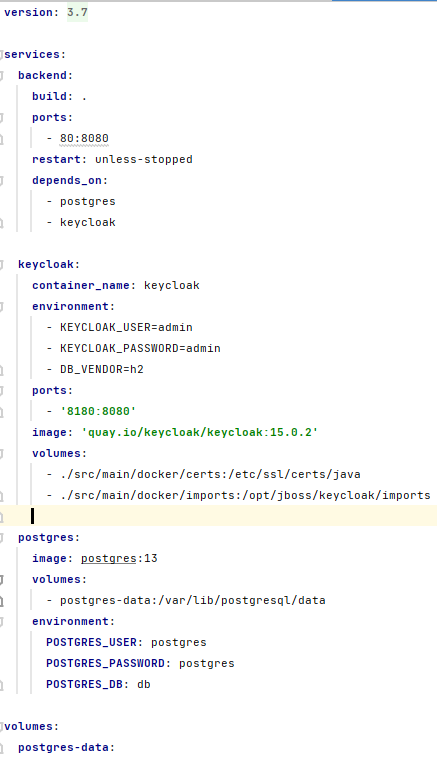
\includegraphics[width=0.6\textwidth]{pics/Bsp_Docker-composeYML.PNG}
  \centering
  \caption{Beispiel für Docker Compose YAML-Datei}
\end{figure}

\subsection{Docker Desktop}
Docker Desktop vereint all diese Komponenten in einer Anwendung, die eine 
benutzerfreundliche Möglichkeit zur Erstellung und gemeinsamen Nutzung von containerisierten 
Anwendungen und Microservices bietet. \cite{noauthor_docker_nodate-3}, \cite{noauthor_install_nodate-1}

\section{Keycloak}
\begin{wrapfigure}{r}{0.3\textwidth}
  \begin{center}
    
\includegraphics[width=0.2\textwidth]{pics/KeyCloak_logopng.png}
    \caption{Keycloak Logo von https://www.gepardec.com/keycloak/}
  \end{center}
\end{wrapfigure}
Keycloak ist ein Open-Source-Identitäts- und Zugriffsmanagement-Tool mit dem Schwerpunkt auf 
modernen Anwendungen wie Single-Page-Anwendungen, mobilen Anwendungen und REST-APIs.
Mit der Verwendung von Keycloak authentifizieren sich Benutzer mittels des Keycloak und nicht mit 
individuellen Anwendungen. Das bedeutet, dass keine Login-Formulare, Authentifizierung von Benutzern 
und Speicherung von Benutzern implementiertet werden müssen. Diese Login-Seite kann sogar angepasst werden.
Nach einmaligen Einloggen bei Keycloak, müssen sich die Benutzer nicht erneut anmelden, um auf 
eine andere Anwendung zuzugreifen. Dasselbe gilt auch für die Abmeldung. Mit der Verwendung von
Single-Sign-Out müssen sich Benutzer nur einmal abmelden um von allen Anwendungen, 
die den Keycloak benutzen, abgemeldet zu werden.  
\newline
\newline
Eine zusätzliche Funktion des Keycloak ist die eingebaute Unterstützung, um sich mittels LDAP mit 
bestehenden Active-Directory-Servern zu verbinden. 
Docker stellt ein Image für Keycloak zur Verfügung. \cite{noauthor_keycloak_nodate-1}, \cite{noauthor_quarkus_nodate}, \cite{noauthor_keycloakkeycloak_nodate}, \cite{noauthor_keycloak_2022}, \cite{noauthor_mit_2020}

\subsection{LDAP}
LDAP oder ausgeschrieben Lightweight Directory Access Protocol ist ein Softwareprotokoll, 
das Daten speichert und sortiert, um sie leicht auffindbar zu machen. Bei den Daten kann es 
sich um beliebige Informationen über Geräte oder Benutzer handeln, die in Verzeichnissen 
gespeichert sind. LDAP ist das Protokoll, das von Servern verwendet wird, um mit den 
Verzeichnissen vor Ort zu kommunizieren.
\newline
\newline
Der Hauptnutzen von LDAP besteht darin, als zentraler Mittelpunkt für die Authentifizierung und 
Autorisierung zu dienen. LDAP hilft dabei Benutzernamen und Kennwörter zu speichern und später 
wieder abrufbar zu machen, zum Beispiel wenn ein Benutzer versucht, auf eine LDAP-fähige Anwendung 
zuzugreifen. Mithilfe der in LDAP gespeicherten Anmeldeinformationen 
wird der Benutzer authentifiziert.
\newline
\newline
In LDAP können auch Benutzerattribute gespeichert werden, die bestimmen, worauf der Benutzer 
zugreifen darf. Obwohl LDAP und Active-Directory (AD) häufig synonym verwendet werden, 
handelt es sich um zwei verschiedene Arten von Software, die jedoch zusammenarbeiten können. \cite{bar_was_nodate}, \cite{noauthor_lightweight_nodate}, 

\subsection{Active-Directory}
Active-Directory (AD) ist eine Datenbank und bietet eine Reihe von Diensten, die Benutzer mit den 
Netzwerkressourcen verbinden. Die Datenbank beziehungsweise das Directory enthält wichtige Informationen 
über Ihre Umgebung, zum Beispiel welche Benutzer und Computer es gibt und wer was tun darf. \cite{noauthor_active_nodate}, \cite{noauthor_lightweight_2022}, \cite{noauthor_active_nodate-1}, \cite{noauthor_was_nodate-8}

Active-Directories bestehen aus drei Hauptebenen: 
\begin{enumerate}
  \item Domänen
  \item Bäume
  \item Wälder
\end{enumerate}

Eine Domäne ist eine Gruppe zusammengehöriger Benutzer, Computer und anderer Objekte. 
Mehrere Domänen können zu einem Baum (tree) zusammengefasst werden, und mehrere Bäume können zu 
einer Gesamtstruktur (auch Forest genannt) gruppiert werden.

\subsection{Login Prozess}
\begin{figure}[H]
  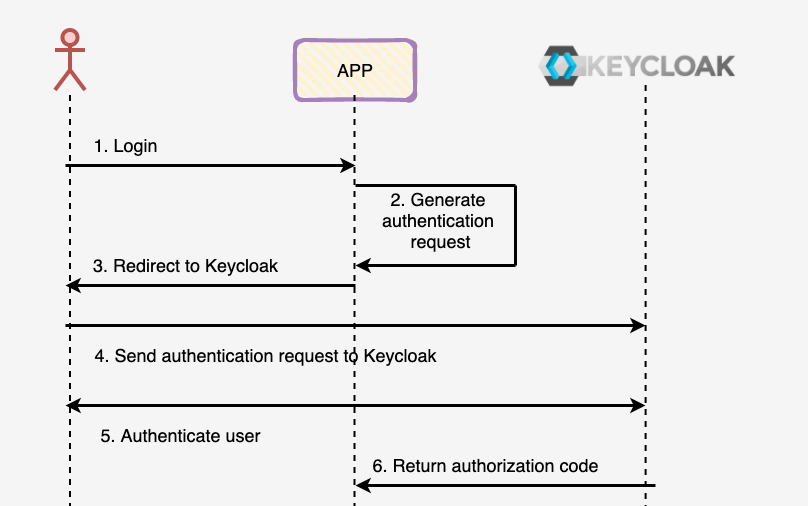
\includegraphics[width=0.8\textwidth]{pics/Keycloak_Auth.png}
  \centering
  \caption{Login Prozess von https://medium.com/codex/introduction-to-keycloak-227c3902754a}
  \label{fig:keycloak1}
\end{figure}

In der Abbildung (siehe Abb. \ref{fig:keycloak1}) wird der Login-Prozess des KeyCloak vereinfachend dargestellt.
\begin{enumerate}
  \item Der Benutzer klickt auf einen Login-Button
  \item Die Anwendung generiert eine Authentifizierungsanfrage.
  \item Die Authentifizierungsanforderung wird an den Benutzer gesendet.
  \item Der Keycloak zeigt dem Benutzer die Anmeldeseite an. Der Benutzer gibt seinen Benutzernamen und sein Passwort ein und schickt das Formular ab
  \item Keycloak überprüft die Anmeldedaten und erstellt daraufhin einen Autorisierungscode, der an die Anwendung zurückgeschickt wird
  \item Autorisierungscode wird gegen das ID-Token und das Refresh-Token ausgetauscht
\end{enumerate}

\subsubsection{JSON-Web-Token (JWT)}
Der Keycloak sendet standardmäßig ein signiertes JSON-Web-Token (JWT).
JSON Web Token (JWT) ist ein offener Standard, der eine kompakte Methode zur sicheren 
Übertragung von Informationen zwischen Parteien in Form eines JSON-Objekts ermöglicht. 
Es wird hauptsächlich für Authentifizierung und Informationsaustausch verwendet.
Diese Informationen können überprüft werden und sind vertrauenswürdig, da sie digital signiert werden.
JWTs können aber auch verschlüsselt werden, um die Geheimhaltung zwischen den Parteien zu gewährleisten. \cite{auth0com_jwtio_nodate}, \cite{noauthor_json_nodate}, \cite{noauthor_json_nodate-1}
 
\subsection{Admin Console}
Über die Admin Konsole können alle Aspekte des Keycloak-Servers zentral verwaltet werden.
Die verschiedene Einstellungen können hier getroffen und Funktionen aktiviert und deaktiviert werden. 
Weiters können Identitäts-Brokering und Benutzer-Föderation konfiguriert werden. Zudem besteht die Möglichkeit 
Anwendungen und Dienste zu erstellen und zu verwalten und feinkörnige Autorisierungsrichtlinien zu definieren.
Einstellungen von Benutzer, einschließlich Berechtigungen und Sitzungen können ebenfalls getroffen werden. \cite{noauthor_keycloak_nodate}, \cite{noauthor_server_nodate}

\begin{figure}[H]
  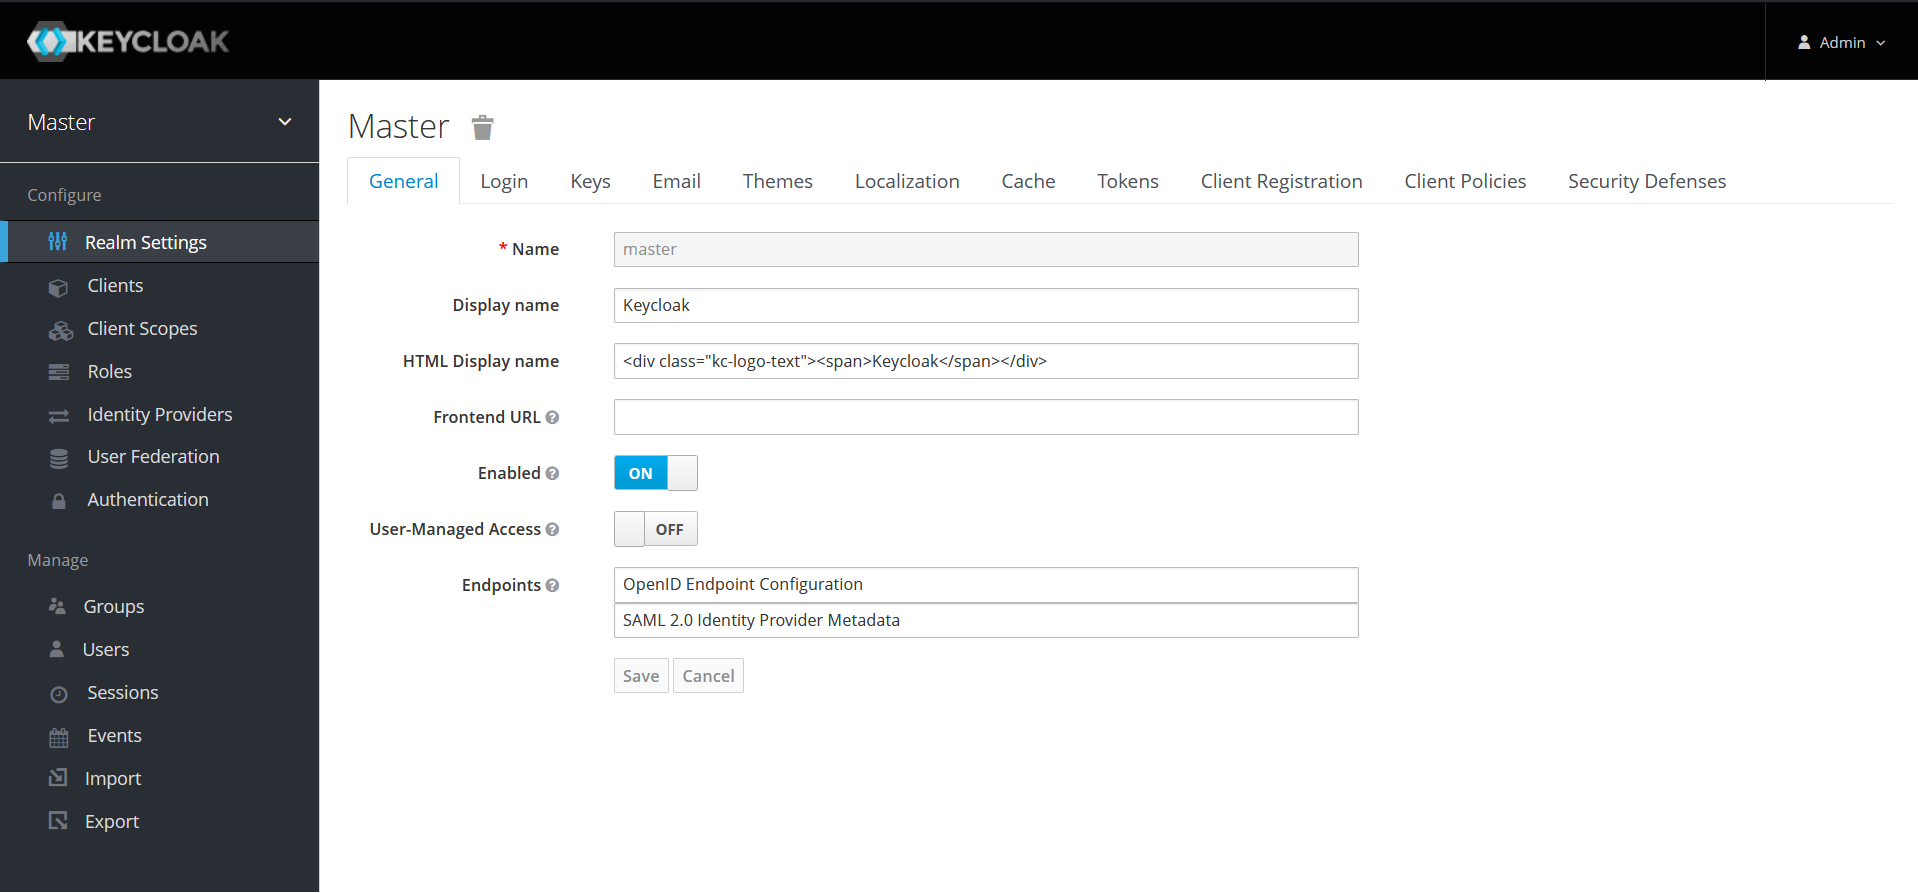
\includegraphics[width=1.0\textwidth]{pics/Keycloak_AdminConsole.PNG}
  \centering
  \caption{Admin Console}
\end{figure}

\subsection{Keycloak Konto-Konsole}
Die Konsole ist für Benutzer. Dort können sie ihr Konto verwalten, z.B. ihr Profil und ihr 
Passwort aktualisieren.

\section{Traefik}
\label{cha:treafik}
\setauthor{Raffeiner Christine}
Traefik ist ein Open Source Edge Router, der die Veröffentlichung von Diensten vereinfacht. 
Der Router empfängt Anfragen stellvertretend für das System und findet heraus, welche Komponenten für deren Bearbeitung 
zuständig sind. Traefik ist kompatibel mit allen wichtigen Cluster-Technologien wie Kubernetes, Docker, Docker Swarm, AWS, 
Mesos und Marathon. 
\newline
\newline
Was Traefik neben seinen vielen Funktionen auszeichnet, ist, dass es automatisch Dienste im Netzwerk erkennt, auch wenn diese nachträglich gestartet werden. 
Traefik inspiziert die Infrastruktur des Systems und findet heraus, welcher Dienst für welche 
Anfragen zuständig ist und kann diese in Echtzeit abfangen und anpassen (z.B. https auf http). 
Traefik benötigt keine separate Konfigurationsdatei um das System zu verwalten und zu synchronisieren: 
Alles geschieht automatisch und in Echtzeit ohne Neustarts und Verbindungsunterbrechungen. \cite{noauthor_traefik_nodate}, \cite{noauthor_traefiktraefik_nodate}
\begin{figure}[H]
  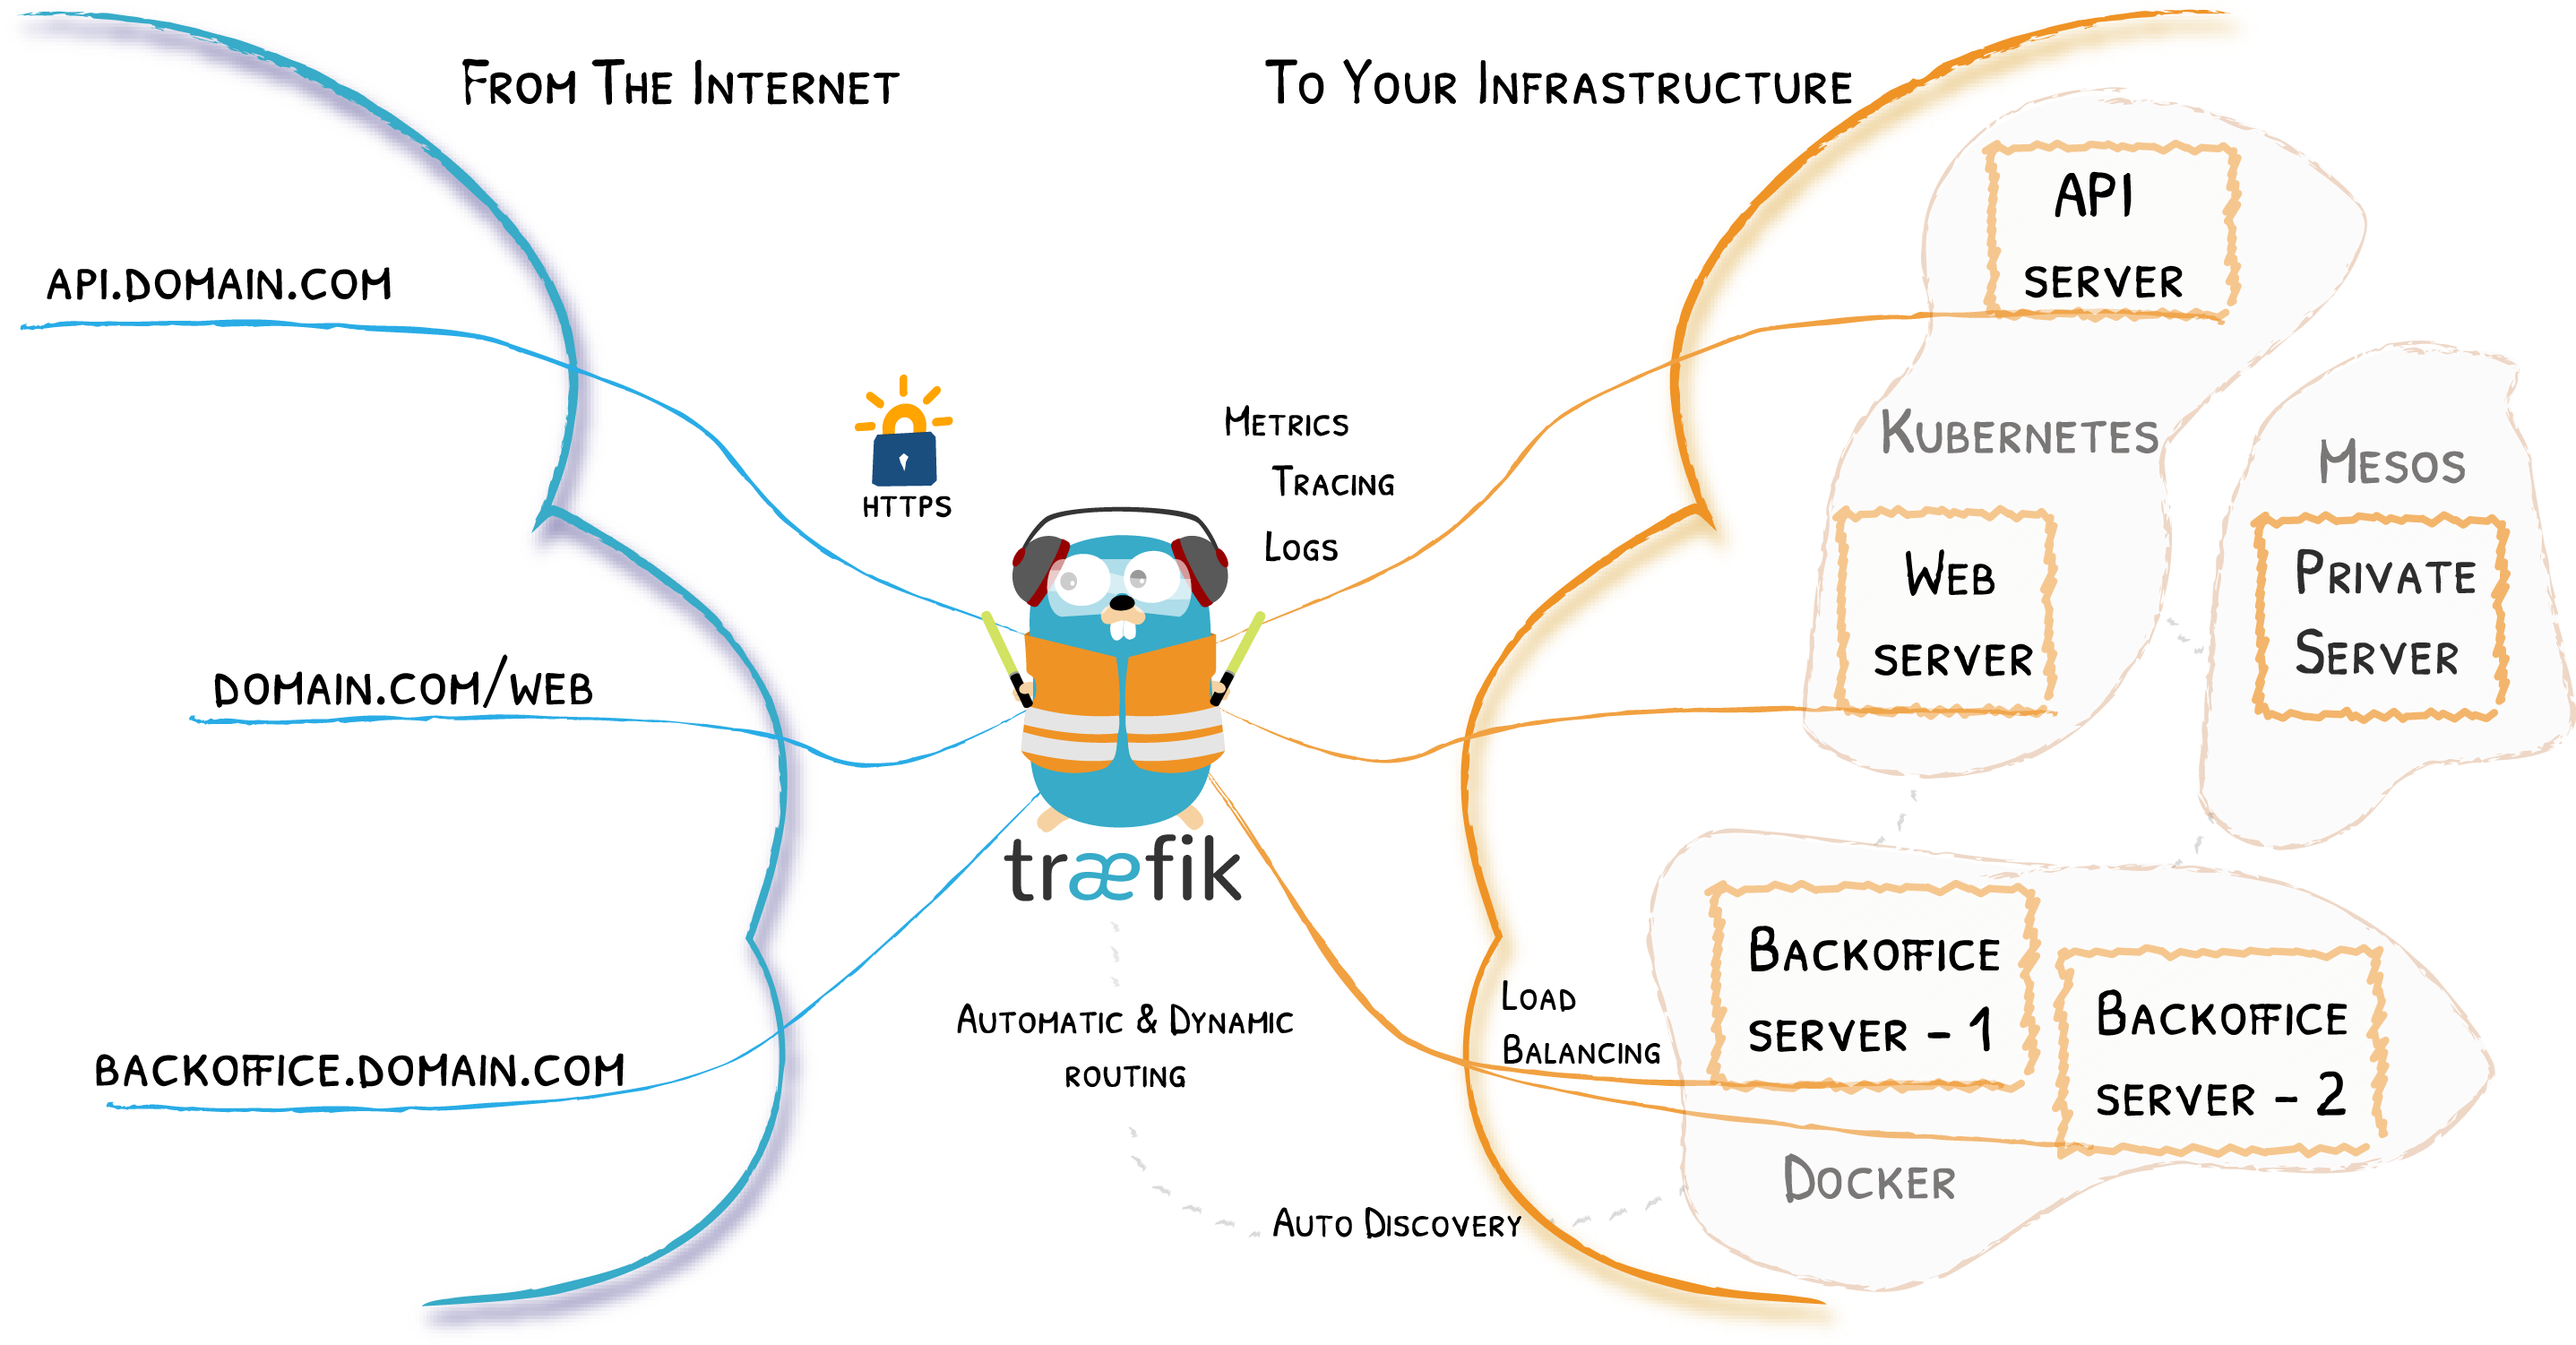
\includegraphics[width=0.9\textwidth]{pics/traefik-architecture.png}
  \centering
  \caption{Funktionsweise Traefik}
\end{figure}

\section{PlantUML}
\label{chap:plantuml}

\begin{figure}[!htb]
        
\includegraphics[width=0.2\textwidth]{pics/PlantumlLogo.png}
        \centering
        \caption{PlantUML Logo source: \cite{noauthor_plantuml_nodate}}
\end{figure}
PlantUML ist ein Open-Source-Werkzeug, mit dem Benutzer/innen Diagramme aus einer einfachen Textsprache 
erstellen können. Neben verschiedenen UML-Diagrammen unterstützt PlantUML auch verschiedene andere 
Formate für die Softwareentwicklung. \cite{noauthor_plantuml_2022}

\subsection{PlantUML integration}
Das Plugin PlantUML integration wird von IntelliJ verwendet um die PlantUML-Dateien anzuzeigen und zu erstellen.
Das Plugin bietet Code-Navigation und Hervorhebung. \cite{noauthor_plantuml_nodate}

\section{Markdown}
\label{chap:markdown}
\begin{figure}[!htb]
        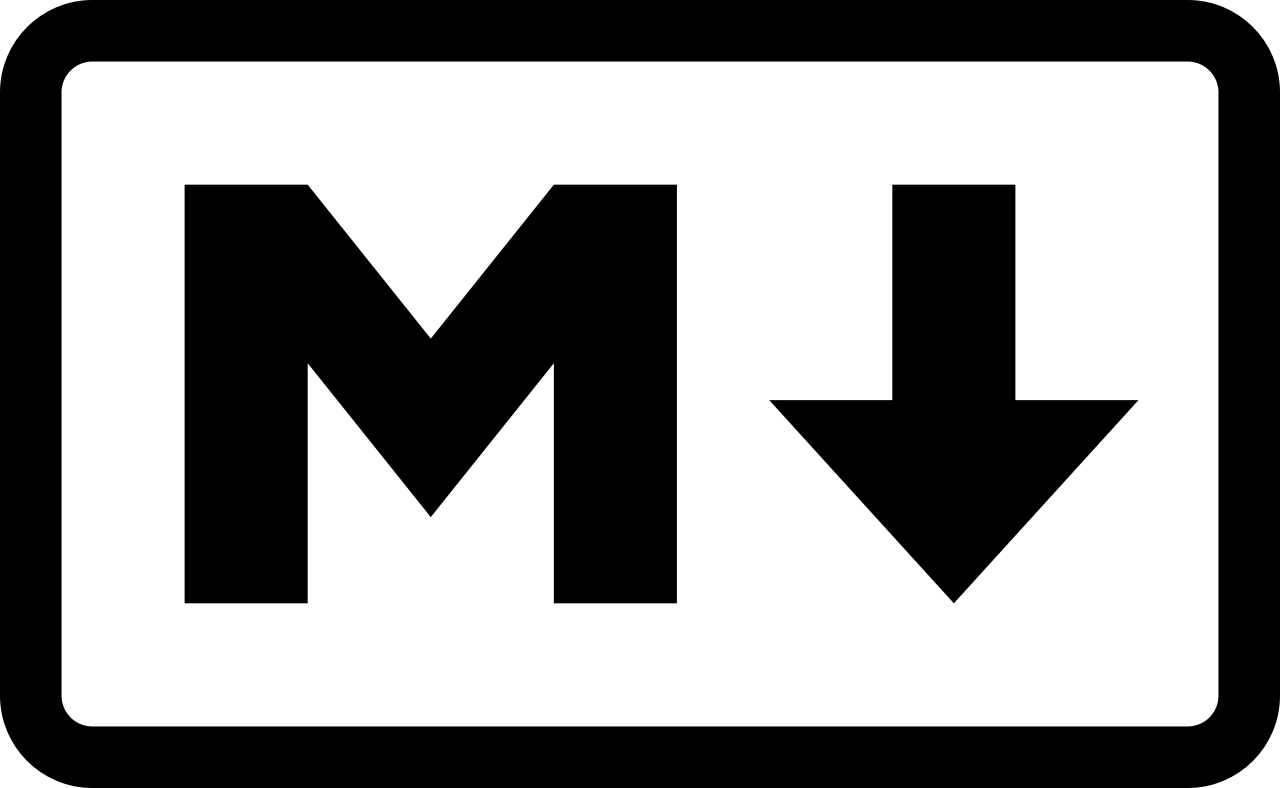
\includegraphics[width=0.2\textwidth]{pics/MarkdownLogo.png}
        \centering
        \caption{Markdown Logo 
        source: \cite{noauthor_markdown_2021} }
\end{figure}

Markdown ist eine leichtgewichtige Auszeichnungssprache, mit der 
Formatierungselemente zu Textdokumenten im Klartext hinzufügen werden können. \cite{noauthor_markdown_2021}, \cite{noauthor_markdown_nodate}

\section{Java}
\setauthor{Weissengruber Nina}
\begin{wrapfigure}{r}{0.3\textwidth}
    \begin{center}
      
\includegraphics[width=0.2\textwidth]{pics/Java_Logo.png}
      \caption{Java Logo ~\cite{java_logo}}
    \end{center}
\end{wrapfigure}
Java ist eine objektorientierte Programmiersprache, die in vielen Teilen der Informatik verwendet wird. 
Java als Programmiersprache dient vor allem zum Formulieren von Programmen. Anfangs liegen die Programme in 
Quellcode, also in für Menschen verständlichen Text vor. Mithilfe des Java-Compilers wird der Quellcode in für
Maschinen verständlichen Bytecode übersetzt. Dieser Quellcode wird dann über die Java Virtual Machine (JVM)
ausgeführt. ~\cite{java}
\newline
\newline
Ein großer Vorteil von Java ist die Plattformunabhängigkeit. Zum Ausführen der Programme oder Anwendungen
wird kein bestimmtes Betriebssystem benötig sondern lediglich die Java-Laufzeitumgebung (JRE).
Diese Laufzeitumgebung ist bereits auf vielen Computern mit verschiedenen Betriebssystemen vorinstalliert, 
wodurch die Plattformunabhängigkeit gegeben ist. Die Plattformunabhängigkeit wird auch durch die Java
Virtuell Machine (JVM) realisiert. ~\cite{java_biteno}
\subsection{Java Runtime Environment}
Die Java Runtime Environment (JRE) oder auch Java Laufzeitumgebung oder Java Runtime ist Teil des Java 
Development Kits (JDK).
\newline
\newline
Eine Laufzeitumgebung verhält sich wie ein kleines Betriebssystem und stellt alle notwendigen
Funktionalitäten für die Ausführung eines Programmes bereit. Die Laufzeitumgebung lädt Anwendungen und
lässt diese auf einer Plattform laufen, auf der alle notwendigen Ressourcen für einen 
betriebsystemunabhängigen Betrieb zu Verfügung.
\newline
\newline
Eine laufende Anwendung interagiert über ein Runtime System mit der Laufzeitumgebung. 
Die Laufzeitumgebung wiederum dient als Vermittler zwischen Anwendung und Betriebssystem. 
Die JRE stellt verschiedene Funktionen für Speicher, Netzwerk und Hardware bereit.
Diese Funktionen werden von der Laufzeitumgebung ausgeführt und nicht von der Anwendung und arbeiten 
unabhängig vom Betriebssystem. 
\newline
\newline
Ein großer Vorteil der Laufzeitumgebung ist, dass Programme Zugriff auf alle benötigten Funktionen haben, 
jedoch unabhängig von Betriebssystem arbeiten.
~\cite{java_jre}

\subsection{Java Development Kit}
Das Java Development Kit (JDK) bildet die Grundlage, auf der Anwendungen aufgebaut werden. 
JDK besteht aus verschiedenen Softwarekomponenten und enthält eine Vielzahl von Tools und Dienstprogrammen, 
mit denen verschiedene Aufgaben ausgeführt werden können. 
Die Hauptverwendung von JDK besteht darin, Code von Java-Code in Bytecode zu kompilieren,
wobei die JRE verwendet wird, um den Bytecode auszuführen.
~\cite{java_jdk}

\subsection{Java Virtual Machine}
Die Java Virtual Machine (JVM) ist die zentrale Komponente der Java-Laufzeitumgebung (JRE). 
Die JVM ermöglicht die plattformunabhängige Ausführung von Programmen im Java-Bytecode. 
Die JVM ist eine prozessbasierte VM oder auch ein einfacher virtueller Computer, in dem Java-Bytecode
ausgeführt wird. Die VM übersetzt die Anweisungen des Bytecodes zur Laufzeit in Maschinencode.
\newline
\newline
Ein weiterer Vorteil der JVM ist die Geschwindigkeit und Sicherheit. Da die Java-Programme von den 
Betriebssystemen abgeschottet sind, wird die Sicherheit erhöht, da Zugriffe auf Ressourcen sich genau
kontrollieren lassen.
~\cite{java_jvm}

\section{Quarkus}
\setauthor{Weissengruber Nina}
\begin{wrapfigure}{r}{0.3\textwidth}
    \begin{center}
      
\includegraphics[width=0.4\textwidth]{pics/Quarkus_logo.jpg}
      \caption{Quarkus Logo ~\cite{quarkus_logo}}
    \end{center}
\end{wrapfigure}

Quarkus ist ein Java Framework für JVMs (Java Virtual Machines) und native Kompilierung, um Java-Anwendungen 
für Container und Clouds zu optimieren.
~\cite{quarkus_redhat}

Quarkus unterstützt 2 Modi:
\begin{enumerate}
\item Optimierung des Bytecodes und Ausführen in der JVM

Java Code, der mit Quarkus geschrieben wurde, kann auf der JVM ausgeführt werden.
Es gibt jedoch Vorteile in Hinsicht auf den Speicherverbrauch und die Startzeit der laufenden Anwendung.
Um dies zu ermöglichen, schiebt Quarkus eine Reihe von zeitaufwendigen Schritten in den Build-Prozess.
Unteranderem:

   \begin{itemize}
     \item Laden und Parsen von Konfigurationen
     \item  Scannen des Java-Klassen-Pfades und das Auflösen von Annotationen
     \item  gegebenenfalls das Erstellen von Entitäten-Modellen für Datenanken
   \end{itemize}

   Quarkus führt diese Schritte einmalig durch und speichert die Ergebnisse für einen schnellen Abruf zwischen.
   \newline
   Unter anderem reduziert Quarkus die Menge der zur Laufzeit dynamisch vorliegenden Informationen. 
   Diese Informationen werden durch entsprechende Konstrukte ersetzt, 
   was im Hinblick auf den Einsatz mit Containern sinnvoll ist. 

\item Ausführen als nativer Code nach Kompilierung

Mit der Ahead-of-time-compilation (AOT) wird aus dem Java-Quelltext kein Bytecode erzeugt, 
sondern direkt ausführbarer Maschinencode. Dies bedeutet, dass auf der Ziel-Hardware keine JVM benötigt wird.
\end{enumerate}
~\cite{quarkus_ionos}

\subsubsection{Ahead-of-time compilation}
Bei der Ahead-of-time (AOT) compilation wird der Programmcode bereits zur Compilezeit/Kompilierzeit in Maschinensprache
übersetzt.
\newline
Mithilfe der AOT compilation wird die Startzeit der JVM von Java-Programmen verbessert.
~\cite{ahead_of_time_compilation}

\section{PostgreSQL}
\setauthor{Weissengruber Nina}
\begin{wrapfigure}{r}{0.3\textwidth}
    \begin{center}
      
\includegraphics[width=0.4\textwidth]{pics/postgreSql_Logo.png}
      \caption{PostgreSql Logo ~\cite{postgre_sql_logo}}
    \end{center}
\end{wrapfigure}
PostgreSQL ist ein leistungsstarkes, objektrelationales Open-Source-Datenbanksystem.
PostgreSQL basiert auf dem Client-Server-Modell, dies bedeutet,
dass ein am Server laufender Prozess die Datenbankdateien und deren Verbindungen, 
die von Client zum Server aufgebaut werden, und bearbeitete Anfragen verwaltet.
~\cite{postgre_sql}
\newline
\newline
Ein Vorteil von PostgreSQL ist, dass es ein Open Source System ist. Somit ist der Code frei zugänglich,
daher ist es möglich, PostgreSQL zu nutzen oder so zu verändern und implementieren,
wie es aktuell für einen von Vorteil ist. Weites ist es möglich, die PostgreSQL Datenbank zu skalieren und
somit kann die Datenbank auf die Größe der Anwendung angepasst werden.
~\cite{postgre_sql_cybertec}

\section{Rest-API}
\setauthor{Weissengruber Nina}
Representational State Transfer - Application Programming Interface (Rest-API) ermöglicht den Austausch von
Informationen, die sich auf unterschiedlichen Systemen befinden. Eine Rest-API ist zustandslos, dies bedeutet,
dass Aufrufe unabhängig voneinander erfolgen und jeder Aufruf alle Daten enthält, 
die erforderlich sind für eine erfolgreiche Durchführung.
~\cite{rest_api_ryte}
\newline
\newline
Außerdem baut Rest-API auf bestehende Systeme und Funktionen des Hypertext Transfer Protocol (HTTP) auf. 
Somit können Rest-basierte Interaktionen deren Status über numerische HTTP-Statuscodes kommunizieren. 
Der Vorteil besteht darin, dass REST-APIs diese HTTP-Statuscodes verwenden, um Fehler zu erkennen.
\newline
\newline
Weiters ist Rest-API Sprachunabhängig, dies bedeutet, dass man beim Erstellen von Restful-APIs oder 
Webdiensten jegliche Sprache verwenden kann, die HTTP verwendet. 
~\cite{rest_api_tech_target}
\newline
\newline
\begin{figure}[!htb]
  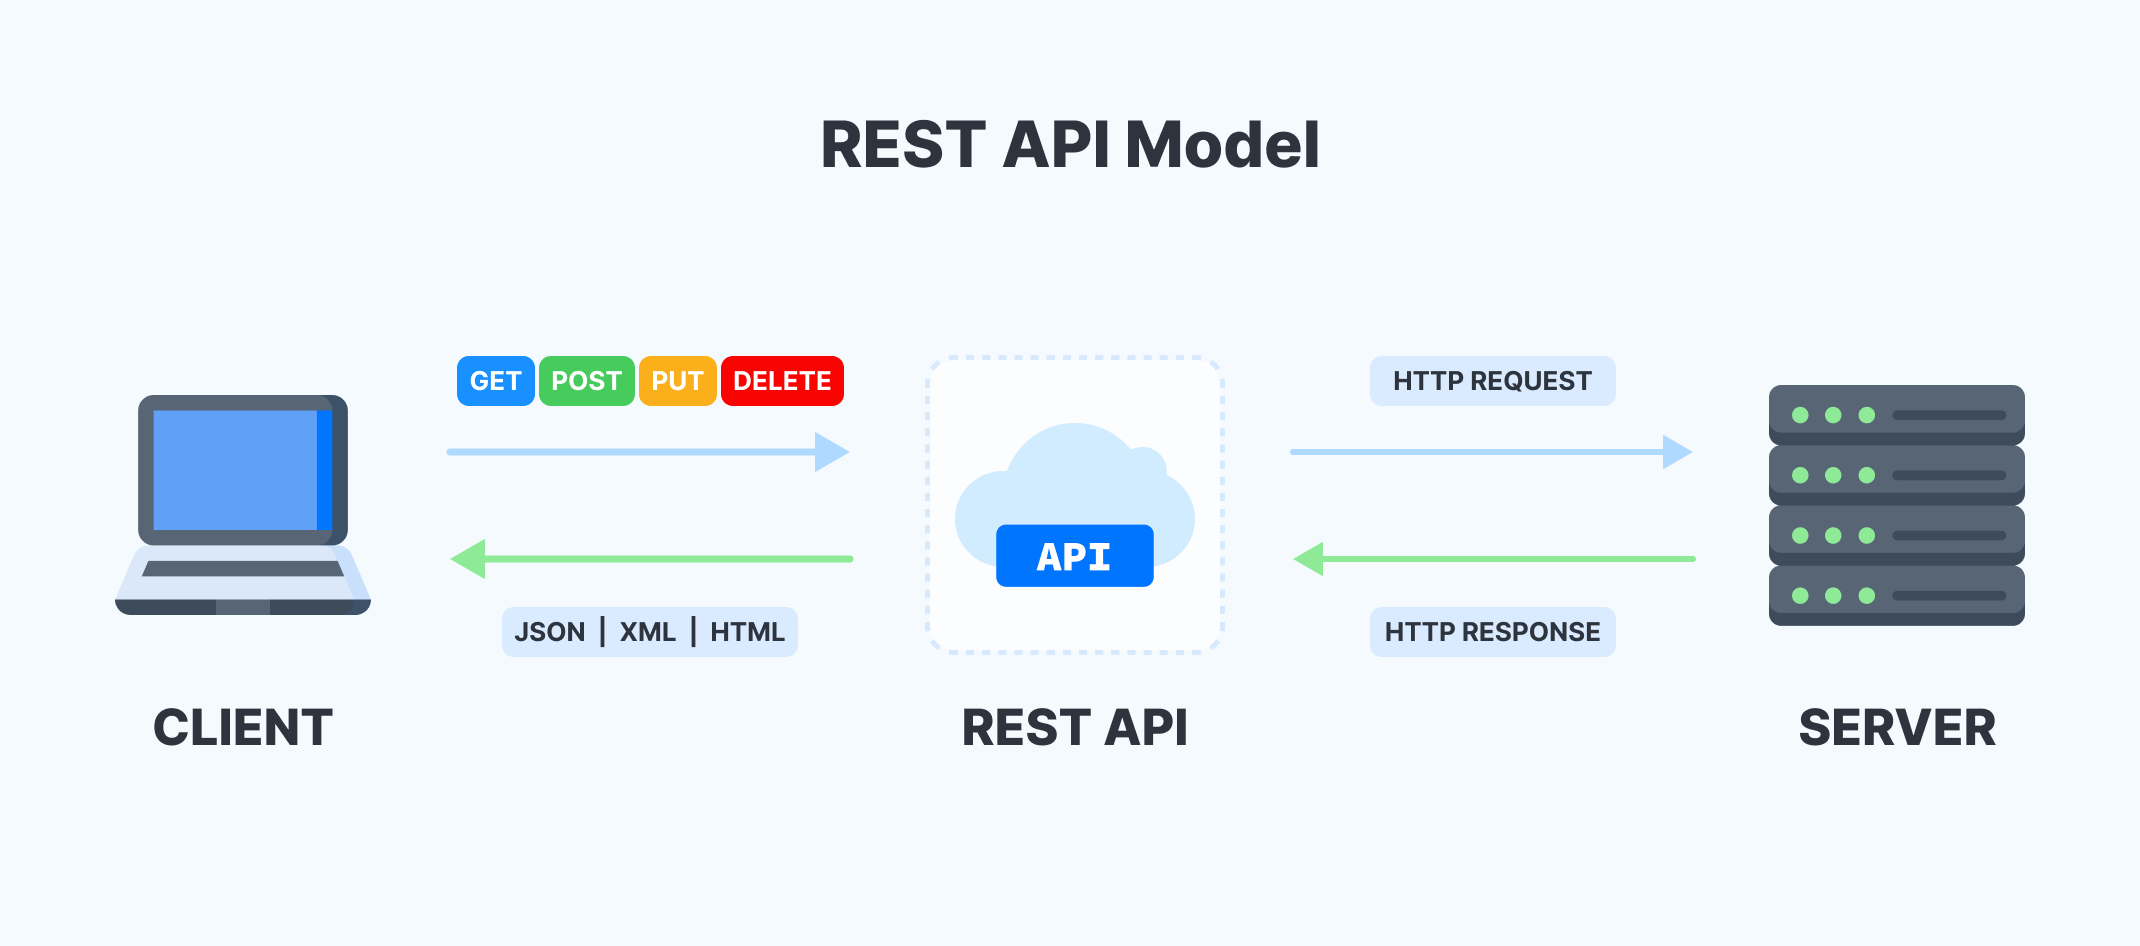
\includegraphics[width=0.8\textwidth]{pics/api-rest-model.png}
  \centering
  \caption{Rest-API Model ~\cite{rest_api_model}}
\end{figure}
\newline
Der Client schickt mittels HTTP-Request Methoden Anfragen an die Rest-API, die die Requests an den Client
weiterschicken.
\newline
Der Server sendet einen HTTP-Response an die Rest-API welche die Response an den Client als JSON,
XML oder HTML Datei sendet.

\subsection{API}
Ein Application Programming Interface (API) ist eine Schnittstelle, die verschiedene Programme verbindet
und die Datenübertragung und den Austausch von Anweisungen zwischen Programmteilen standardisiert.
\newline
APIs bieten verschiedene Anwendungsbereiche, über welche unterschiedliche Aufgaben ausgeführt werden können.
\newline
Es gibt vier verschiedene Arten von APIs:
\begin{itemize}
  \item Funktionsorientierte APIs
  \item Dateiorientierte APIs
  \item Protokollorientierte APIs
  \item Objektorientierte APIs
\end{itemize}

Funktionsorientierte APIs sind komplexe Schnittstellen, die es ermöglichen, auf Hardware-Komponenten
zuzugreifen. Dateiorientierte APIs ermöglichen die Verbindung auf Dateiebene und damit können Daten
abgefragt und geschrieben werden. Protokollorientierte APIs werden zur standardisierten Kommunikation 
zwischen Programmen verwendet. Objektorientierte APIs sind flexibel und können in verschiedenen Bereichen 
eingesetzt werden.
~\cite{api}

\subsection{HTTP}
Hypertext Transfer Protocol (HTTP) ist ein Protokoll, mit dem Daten in Netzwerken übertragen werden. 
HTTP ist standardisiert und definiert, wie Webclient und Server miteinander kommunizieren, 
damit vom Client angeforderte Daten geladen und angezeigt werden.
\newline
\newline
HTTP definiert zwei unterschiedliche Arten von Nachrichten

\begin{itemize}
  \item Anfrage (Request)
  \item Antwort (Response)
\end{itemize}

Diese Nachrichten bestehen aus einem HTTP-Header und einem HTTP-Body. 
Im Header sind Meatinformationen enthalten und im Body befinden sich die Daten, 
die an den Client geschickt werden.
\newline
\newline
Zur Übertragung von Daten zwischen Server und Client wird das TCP/IP-Protokoll verwendet. 
Fordert der Client über TCP ein Dokument an, wird eine Antwort (Response) vom Server versendet,
dabei wird auch ein HTTP-Statuscode mitgesendet. Mithilfe des Statuscodes wird Auskunft darüber gegeben,
ob die Anfrage erfolgreich war. Je nachdem, ob es erfolgreich war oder nicht wird ein dreistelliger
HTTP-Code an den Client gesendet.
~\cite{http_ryte}

\subsubsection{HTTP-Statuscodes}
HTTP-Statuscodes zeigen an, ob eine HTTP-Anfrage (Request) erfolgreich abgeschlossen wurde.

Man unterscheidet zwischen folgenden Statuscodes:
\begin{itemize}
  \item Informative Antworten (100-199)
  \item Erfolgreiche Antworten (200-299)
  \item Umleitungen (300-399)
  \item Client-Fehler (400-499)
  \item Server-Fehler (550-599)
\end{itemize}
~\cite{http_statuscode}

\begin{figure}[!htb]
  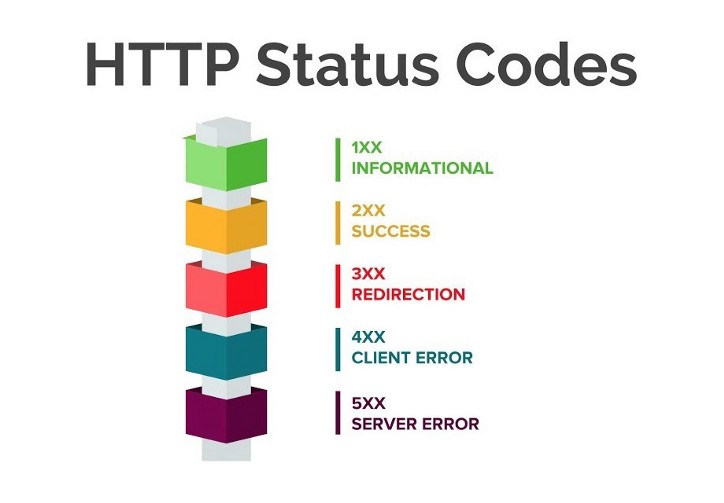
\includegraphics[width=0.8\textwidth]{pics/httpStatusCodes.jpeg}
  \centering
  \caption{HTTP-Statuscodes ~\cite{http_statuscode_pic}}
\end{figure}

\subsubsection{HTTP-Request}
Ein HTTP-Request ist eine Anfrage, die vom Client an den Server gesendet wird.
Die Requests sagen mithilfe von Methoden, Server mit dem Request durchführen soll.
\newline
\newline
Folgende Methoden können in den Requests enthalten sein:
\begin{itemize}
  \item \textbf{"GET"}: Mithilfe der GET-Methode
  fordert der Client Inhalte vom Server an.
  \item \textbf{"POST"}: Mit POST sendet der
  Client Dokumente zum Server.
  \item \textbf{"HEAD"}: Die HEAD-Methode ist
  ähnlich zur GET-Methode, jedoch wird nur der Header eines Dokuments angefordert.
  \item \textbf{"PUT"}: Bei der PUT-Methode sendet der Client Daten zum Server.
  Beziehen sich die mitgeschickten Daten auf eine vorhandene Ressource,
  werden diese aktualisiert, ansonsten neu erstellt.
  \item \textbf{"DELETE"}: Mithilfe der
  DELETE-Methode werden Daten auf dem Server gelöscht.
  \item \textbf{"CONNECT"}: Mit der
  CONNECT-Methode kann ein Tunnel erstellt werden, um auf Websites, die SSL verwenden, zuzugreifen.
  \item \textbf{"OPTIONS"}: Bei der
  OPTIONS-Methode kann der Client Informationen über verfügbare Kommunikationsoptionen abrufen.
  \item \textbf{"Trace"}: Über die TRACE-Methode
  kann der Client Requests verfolgen. 
\end{itemize}

\begin{figure}[!htb]
  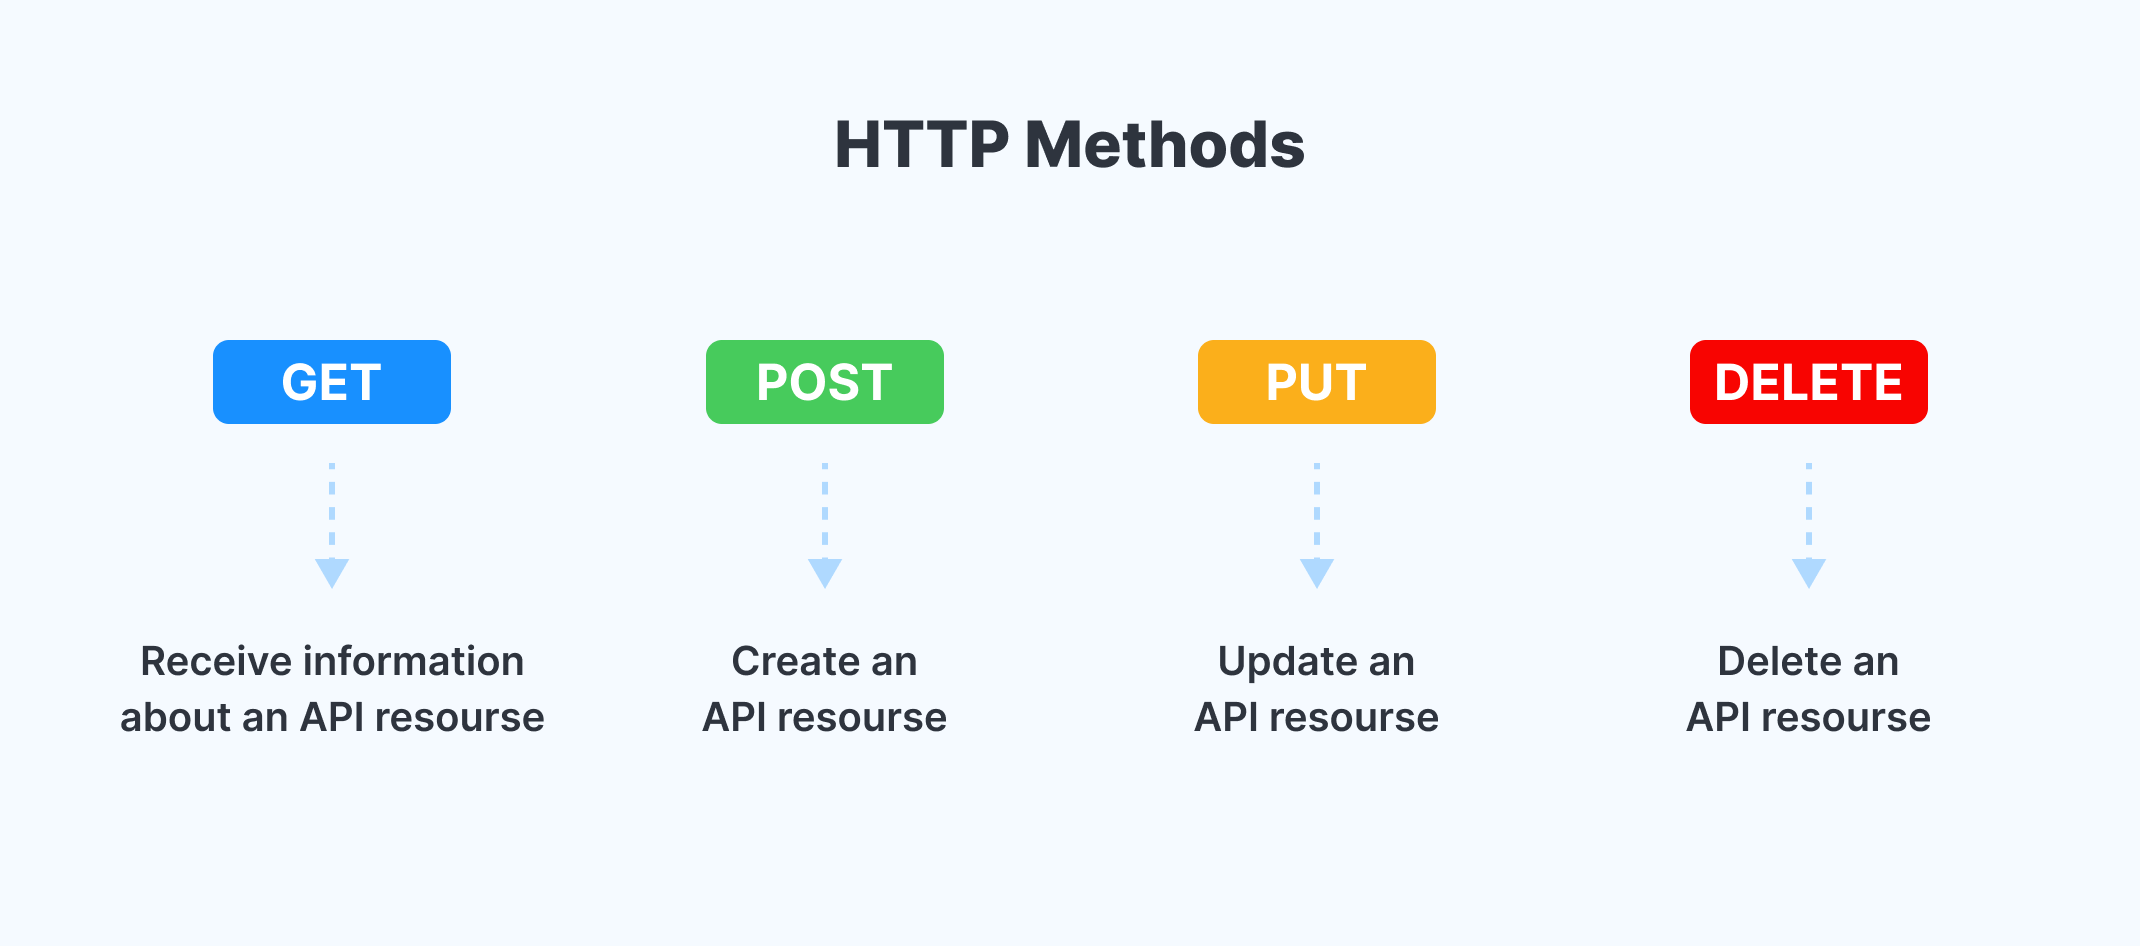
\includegraphics[width=0.8\textwidth]{pics/funktionsweiseRest.png}
  \centering
  \caption{HTTP-Methoden ~\cite{rest_api_model}}
\end{figure}

\subsubsection{HTTP-Response}
Ein HTTP-Response ist eine Antwort oder Meldung, die von Server zum Client gesendet wird. 
Ein HTTP-Response besteht aus einem Header mit optionalen Antwortparametern und einem Body, der
jedoch auch leer sein kann. 
Der Header enthält die Protokollversion, außerdem enthält er auch noch einen Statuscode und einer
Statusmeldung. Der Statuscode der Antwort teilt dem Client mit, ob
die gewünschte Operation vom Server ausgeführt werden konnte.
~\cite{http_response}

\subsubsection{TCP/IP-Protokoll}
Das TCP/IP-Protokoll ist eine Gruppe von Protokollen,
die die Grundlage für das Internet und andere Netzwerke bilden. 
Der Name TCP/IP setzt sich aus den beiden Protokollen Transmission Control Protocol (TCP) und 
Internetprotokoll (IP) zusammen. 
Wobei bei auch bei diesen Protokollen mehrere Protokollen zusammengefasst werden. 
Bei TCP/IP handelt es sich also um keine bestimmte Technik, sondern um eine Gruppierung von Protokollen.
\newline
\newline
Die Protokolle des TCP/IP-Models sind so standardisiert, dass es nicht von Wichtigkeit ist, 
welches Betriebssystem oder welches Gerät man für die Kommunikation über das Netzwerk verwendet.
~\cite{tcp_ip}

\section{Software-Testing}
\setauthor{Weissengruber Nina}
Software-Testing ist der Prozess, um die Funktionalität einer Softwareanwendung zu bewerten. 
Es dient zum Feststellen, ob die entwickelte Software die Anforderungen erfüllt oder nicht.
Es wird also das Ergebnis der Entwicklung getestet.
~\cite{software_testing}

\subsection{Testtechniken}
Man unterscheidet zwischen zwei Testtechniken
\subsubsection{Statische Testtechniken}
Statische Testtechniken dienen dem Überprüfen von Arbeitsergebnissen, ohne diese auf dem Rechner auszuführen.
\newline
Vorteile sind, dass es eine frühe Fehlererkennung gibt und Fehler direkt aufgedeckt werden.
Außerdem verringern sie die Anzahl von dynamischen Tests, welche aufwändiger und teuer sind.
\subsubsection{Dynamische Testtechniken}
Dynamische Testtechniken werden verwendet, um Fehler in der Software zu entdecken.
\newline
~\cite{software_testing_methoden}
Es gibt verschiedene dynamische Testtechniken. Die geläufigsten sind:
\begin{itemize}
  \item \textbf{"Black-Box-Testverfahren"}
  Dabei werden Testfälle nur anhand der Spezifikationen/Anforderungen erstellt, 
  ohne die innere Struktur zu berücksichtigen.
  ~\cite{black_box}
  \item \textbf{"White-Box-Testverfahren"}
  Berücksichtigt im Gegensatz zum Black-Box-Testverfahren das innere des Testobjekts,
  das heißt den Code.
  ~\cite{white_box}
  \item \textbf{"Erfahrungsbasierte Testverfahren"}
  Dabei werden Testfälle anhand von Erfahrungen, Wissen und Intuition der Tester erstellt.
  ~\cite{erfahrungsbasiertes_testen}
\end{itemize}

\subsection{Testarten}
Man unterscheidet zwischen verschiedenen Arten zu testen. Die Entscheidung, welcher Test verwendet werden
soll, hängt von dem Ziel ab, welches der Test erfüllen soll.
\subsubsection{Funktionale Tests}
Funktionale Tests konzentrieren sich auf Funktionen in der Anwendung und überprüfen, 
ob diese ihre Aufgabe richtig erfüllen.
\subsubsection{Nicht-funktionale Tests}
Nicht funktionale Tests überprüfen, wie gut die Anwendung im Ganzen funktioniert.
\begin{itemize}
  \item \textbf{"Performanz/ Effizienz"}
  wird durch Performanztests oder Lasttest geprüft.
  \item \textbf{"Zuverlässigkeit"}
  Zuverlässigkeitstest überprüfen, ob ein Testobjekt über einen bestimmten Zeitraum ein bestimmtes 
  Leistungsniveau unter bestimmten Bedingungen aufrechterhält.
  \item \textbf{"Benutzbarkeit/ Gebrauchstauglichkeit"}
  Benutzbarkeitstests prüfen, wie gut und einfach ein System für den Benutzer zu bedienen ist.
  \item \textbf{"Sicherheitstest"}
  überprüfen, ob System und Daten vor unerlaubten Zugriffen und externen Bedrohungen geschützt sind.
  \item \textbf{"Kompatibilität"}
  Interoperabilitätstest bewerten die Fähigkeit des Softwareprodukts.
  \item \textbf{"Wartbarkeit"}
  wird durch Reviews und werkzeuggeschützte statische Analyse geprüft.
  \item \textbf{"Übertragbarkeit"}
  wird durch Portabilitätstests getestet.
\end{itemize}
~\cite{software_testing_methoden}

\subsection{Unit Test}
Mithilfe von Unit Tests werden Komponenten des geschriebenen Codes überprüft. 
Der Code wird in einzelne Teile isoliert und diese Teile werden auf ihre Funktionalitäten überprüft.
\newline
\newline
Unit Tests sind nach den drei A's der Modultests aufgebaut.
\begin{itemize}
  \item \textbf{"Arrange (Anordnen)"}:
  Beim Arrange werden die Anforderungen definiert, die der Code erfüllen muss.
  \item \textbf{"Act (Handeln)"}:
  Beim Act wird der Test durchgeführt.
  \item \textbf{"Assert (Umsetzung)"}:
  Beim Assert werden die Ergebnisse überprüft. Wenn die Ergebnisse dem entsprechen, was erwartet
  wird, wird der Test validiert.
\end{itemize}
~\cite{unit_test}

\subsection{Smoke Test}
Smoke Test werden als Software-Probelauf bezeichnet. 
In einem kurzen Zeitraum soll die Funktionalität von neuen Funktionen und Anwendungen geprüft werden. 
Das Ziel von Smoke Tests ist es, Fehler zu finden, die später gravierende Probleme auslösen.
~\cite{smoke_test}

\subsection{Regressionstest}
Mithilfe von Regressionstests wird überprüft, ob Änderungen an der Anwendung oder andere dazugehörige
Softwarekomponenten Fehler herbeiführen und ob die Änderungen am Code die Funktionsweise beeinträchtigen 
oder stören.
\newline
\newline
Regressionstests können bei folgende Prozessen erforderlich sein:
\begin{itemize}
  \item beim Einführen von neuen Features
  \item beim Beheben eines Fehlers
  \item beim Refactoring zur Steigerung der Leistung
  \item beim Ändern der Hosting-Umgebung einer Anwendung
\end{itemize}

Regressionstests werden auf einer der folgenden Testebene durchgeführt:
\begin{itemize}
  \item Unit-Tests
  \item Integrationstests
  \item Systemtests
  \item Akzeptanztests
\end{itemize}
~\cite{regressionstests}

\subsection{Integrationstest}
Bei Integrationstests werden Units in Gruppen auf verschiedenste Weise kombiniert und getestet. 
Integrationstests können Probleme von Schnittstellen aufdecken. 
\newline
\newline
Es gibt 2 Methoden zur Durchführung von Integrationstest:
\begin{itemize}
  \item \textbf{"Bottom-up-Methode"}:
  Bottom-up Integrationstests beginnen mit Unit-Test, die gefolgt werden von Tests mit Kombinationen von Units.

  \item \textbf{"Top-down-Methode"}:
  Top-down Integrationstests beginnen damit, die Module höchster Ebene zu testen. Erst dann werden Module niedrigerer Ebenen getestet.

\end{itemize}
~\cite{integrationstests}

\subsection{Systemtests}
Bei Systemtests wird überprüft, wie die verschiedenen Komponenten im vollständigen System oder in der Anwedung
zusammenarbeiten.
\newline
Es gibt verschiedene Arten von Systemtests, welche unterschiedliche Komponenten testen:
\begin{itemize}
  \item \textbf{"Leistungstests:"}
  Geschwindigkeit, Stabilität, Reaktionszeiten
  \item \textbf{"Lasttests"}:
  Latenz, Anzahl der Benutzer
  \item \textbf{"Usability-Tests"}:
  Aufgabenerfolgsrate, Zeit bis Aufgaben erledigt sind
\end{itemize}
~\cite{systemtest}

\subsection{Testframeworks}
Testframeworks sind Richtlinien oder Regeln, die zum erstellen und entwerfen von Testfällen
verwendet werden.

~\cite{testframework}


\begin{spacing}{1}
\chapter{Tools}\label{chapter:tech}
\end{spacing}
\section{Adobe XD}
\setauthor{Raffeiner Christine}
\begin{wrapfigure}{r}{0.3\textwidth}
    \begin{center}
      
\includegraphics[width=0.15\textwidth]{pics/XD_Logo.png}
    \end{center}
\end{wrapfigure}
Adobe XD ist eine kostenpflichtige vektorbasierte Design-Plattform für die Erstellung von Wireframes, Animations- und Interaktions-Design, 
User Interface Design und Prototypen und gilt weiters als All-in-One-Tool. Adobe XD erlaubt es Komponenten als eine Art Template anzulegen 
und diese zur Wiederverwendung und Synchronisierung gängiger Elemente wie zum Beispiel Buttons und Navigationssymbole zu verwenden.
Verändert man nun eine erstellte Hauptkomponente im Nachhinein, werden alle zugehörigen Änderungen automatisch in allen Instanzen angezeigt.
Mit Komponentenzuständen können allerdings Variationen für eine einzelne Komponente erstellt werden. Zum Beispiel kann eine andere 
Hintergrundfarbe im Hover-Zustand (Mauszeiger liegt über dem Element) bestimmt werden.
\newline
\newline
Eine weitere Funktion Responsive Resize erkennt Layouts und passt das Design für andere Formate automatisch an. Adobe XD bietet ebenfalls die Verwendung von Plug-ins für 
die verschiedensten Funktionen, wie zum Beispiel die Verwendung von Icons, an. Um einen funktionierenden Prototyp zu erstellen 
kann auf die Verwendung von Ankerlinks nicht verzichtet werden, da nahtlose Übergänge und eine Navigation von Seite zu Seite dafür unabdinglich sind. \cite{noauthor_adobe_nodate}, \cite{noauthor_was_nodate}

\section{Oracle SQL-Developer}
\setauthor{Raffeiner Christine}
\label{chap:sqldeveloper}
Oracle SQL Developer ist eine kostenlose, integrierte Entwicklungsumgebung, für die 
Entwicklung und Verwaltung von Datenbanken. SQL Developer bietet eine vollständige 
Ende-zu-Ende-Entwicklung von PLSQL- und SQL-Anwendungen, ein Arbeitsblatt für die Ausführung von 
Abfragen und Skripten, eine Datenbankadministrationskonsole für die Verwaltung der Datenbank, eine 
Berichtschnittstelle und eine vollständige Datenmodellierungslösung den Data Modelers. \cite{noauthor_was_nodate-1}

\subsection{Data Modeler}
Oracle SQL Developer Data Modeler ist ein kostenloses, grafisches Tool, 
dass die Datenmodellierungsaufgaben vereinfacht. 
Mit dem Data Modeler können Benutzer/innen logische, relationale, physische und 
mehrdimensionale Datentypenmodelle erstellen, durchsuchen und bearbeiten. 
Der Data Modeler bietet Forward- und Reverse-Engineering-Funktionen und unterstützt die 
gemeinsame Entwicklung durch integrierte Quellcodekontrolle. \cite{noauthor_data_nodate}

\begin{spacing}{1}
\chapter{Ausgewählte Aspekte}
\end{spacing}
\section{Besonders gut gelöste Programmteile}
\subsection{Internationalization}
\setauthor{Raffeiner Christine}
\begin{lstlisting}[language=HTML, caption=Internationalization-Makierung im HTML, label=lst:Internationalization_HTML]
  <mat-label i18n="label text|Question text">Fragetext eingeben</mat-label>
  <mat-card-title i18n="Title|card title" >Frage {{administration.question.sequenceNumber}}</mat-card-title>
\end{lstlisting}

Texte, die eine Übersetzung bekommen sollen, werden mit der Kennzeichnung i18n versehen, kurz für Internationalization.
Nach der Kennzeichnung können noch zusätzliche Informationen in der Form von i18n=\dq <Bedeutung> | <Beschreibung>\dq  für die automatische Übersetzung angegeben werden. 
In diesem Beispiel wurde keine automatische Übersetzung verwendet, trotzdem wurden zusätzliche Attribute angeben um im Falle eines Umstiegs schneller wechseln zu können.
\newline
\newline
\begin{lstlisting}[language=XML, caption=xliff-Datei, label=lst:xliffDatei]
  <?xml version="1.0" encoding="UTF-8" ?>
  <xliff version="1.2" xmlns="urn:oasis:names:tc:xliff:document:1.2">
  <file source-language="en" datatype="plaintext" original="ng2.template">
    <body>
      <trans-unit id="3292363768460657245" datatype="html">
        <source>Richtige Antwort</source>
        <target>Right Answer</target>
        <context-group purpose="location">
          <context context-type="sourcefile">src/app/answer-option-erstellen/answer-option-erstellen.component.html</context>
          <context context-type="linenumber">7</context>
        </context-group>
        <note priority="1" from="description">right answer</note>
        <note priority="1" from="meaning">checkbox text</note>
      </trans-unit>
      <trans-unit id="878423452191694276" datatype="html">
        <source><x id="INTERPOLATION" equiv-text="{{this.questions.length}}"/> Fragen</source>
        <target><x id="INTERPOLATION" equiv-text="{{this.questions.length}}"/> Question</target>
        <context-group purpose="location">
          <context context-type="sourcefile">src/app/answer-survey/answer-survey.component.html</context>
          <context context-type="linenumber">4</context>
        </context-group>
        <note priority="1" from="description">qestion anz</note>
        <note priority="1" from="meaning">headline text</note>
      </trans-unit>
      ...
\end{lstlisting}

Durch die Ausführung des Befehls \textit{ng xi18n --output-path src\textbackslash locale} werden alle Texte mit dem Kennzeichen ibn18 in eine XLF-Datei
extrahiert. In der Datei wird zuerst angegeben in welcher Form sie geschrieben ist. In diesem Fall ist es eine XLF-Datei mit der Version 1.2 (Angular Standard). (Zeile 2)
\newline
\textit{source-language=\dq en\dq} gibt die Sprache an. (Zeile 3)
\newline
Eine \textit{<trans-unit>} wird für jeden mit einer Kennzeichnung versehenen Text generiert. (Zeile 5)
\newline
In \textit{<source>} steht der Originaltext, der angegeben wurde. (Zeile 6)
\newline
Der Text der nun als Übersetzung gilt muss umklammert von \textit{<target> <\textbackslash target>} für jede \textit{<trans-unit>} selbst übersetzt und unter \textit{<source>} eingefügt werden. (Zeile 7)
\newline
\newline
\begin{lstlisting}[language=TypeScript, caption=Konfigurieren der Sprachen im angular.json, label=lst:Angular.json]
  "i18n": {
    "sourceLocale": "de",
    "locales": {
      "en": "src/locale/language_source.eng.xlf"
      }
    ...
    "en":{
    "localize": ["en"]
     },
    "de":{
      "localize": ["de"]
    },
    ...
\end{lstlisting}
Zum Schluss muss der Applikation noch mittgeteilt werden, wo die Ausgangssprache Datei liegt (Zeile 4) und in welcher Sprache diese angegeben ist. 
Zeile 7 und 10 sind Kürzel, die später für das Starten der Applikation wichtig sind.
\newline
\newline
Es ist zu beachten, dass nach diesen Änderungen beim Starten der Applikation immer anzugeben ist welche Sprache verwendet werden soll.
Beispielsweise: \textit{ng serve --configuration=de} oder \textit{ng serve --configuration=en}
Durch kleine Änderungen im package.json kann auch automatisiert eine bestimmte Sprache gestartet werden.

\begin{lstlisting}[language=TypeScript, caption=automatisches Starten der deutschen Sprache, label=lst:package.json]
  "scripts": {
    "ng": "ng",
    "start": "ng serve --configuration=de",
    ...
\end{lstlisting}
Mittels \textit{npm start} wird nun automatisch die deutsche Version der Applikation gestartet.

\subsection{Angular-CSS bearbeiten}
\setauthor{Raffeiner Christine}
\begin{lstlisting}[language=TypeScript, caption=Semi-Transperentes Eingabefeld, label=lst:Ng-deep]
::ng-deep .mat-form-field-appearance-fill .mat-form-field-flex {  
    background: rgba(255, 255, 255, 0.5);
}
\end{lstlisting}
Um den Hintergrund einer Material-Komponente Mat-Form-Field (eine Komponente die Formularelemente
einschließt) halbtransparent zu machen wurde ng-deep verwendet.
\newline
\newline
Ng-deep ermöglicht den Zugriff auf DOM-Elemente, in nicht selbstgeschriebenen Komponenten.
Im Beispiel von Angular Material (oder eine andere Bibliothek eines Drittanbieters wie Materials), befinden 
sich die Elemente außerhalb des Bereichs (wie zum Beispiel Eingabefelder), und lassen keinen direkten Zugriff mit CSS auf diese Elemente 
zu. Ng-deep ermöglicht diesen Zugriff. Mehr Infos zu Angular Material befinden sich im Kapitel \ref{chap:materials}.

\subsection{Keycloak}
\setauthor{Raffeiner Christine}
Mittels des Keycloak können sich die Benutzer der Applikation mit gewohnten Anmeldeinformationen anmelden.
\begin{lstlisting}[language=TypeScript, caption=Konfiguration des Keycloaks, label=lst:Konfiguration-Keycloak]
{
  "backendApiUrl": "http://localhost:8080/api",
  "keycloakUrl": "http://localhost:8180/auth/realms/School"
}
\end{lstlisting}
Für die Anbindung des Keycloaks an das Frontend muss zuerst festgelegt werden, unter welcher URL sich der KeycloakService und das Backend befinden.
\newline
\newline
\begin{lstlisting}[language=TypeScript, caption=Aufrufen des Logins, label=lst:Initialisierung Login]
  openLogin(){
    this.config.init().then(() => this.authenticationService.initializeLogin())
  } 
\end{lstlisting}
Wird nun das Login aufgerufen wird der Authentifikations-Service initialisiert.
\newline
\newline
\begin{lstlisting}[language=TypeScript, caption=Initialisierung des AuthenticationService, label=lst:authenticationService]
  init(): Promise<any> {
    return this.httpClient
      .get<Config>('/assets/config.json')
      .pipe(
        tap(config => {
          this.config = config;
          authModuleConfig.resourceServer.allowedUrls!.push(config.backendApiUrl);
        })
      )
      .toPromise();
  }
\end{lstlisting}
Mit der Initialisierung werden die angegebenen Konfigurationsdateien ausgelesen und die angegeben URLs zum Weiterleiten zugelassen.
\newline
\newline
\begin{lstlisting}[language=TypeScript, caption=Aufrufen des Authentifikationswächters, label=lst:URLRouten]
  const routes: Routes = [
    {path: '', component: StartseiteComponent, pathMatch: "full"},
    {path: '', canActivateChild: [AuthGuard], children: [
      //{path: '', redirectTo: '/dashboard', pathMatch: 'full'},
      {path: 'dashboard', component: DashboardComponent},
      {path: 'fragebogen-erstellen', component: FragebogenErstellenComponent},
      {path: 'dashboard/fragebogen-editieren/:id', component: EditQuestionnaireComponent}
    ]},
    {path: 'answerSurvey', component: AnswerSurveyComponent},
    {path: 'startseite', component: StartseiteComponent},
    {path: '**', component: StartseiteComponent}
  ];
\end{lstlisting}
Man wird nicht nur mit dem Klick auf den Login-Knopf zum Anmelden auf den Keycloak weitergeleitet. Will man auf 
Unterseiten, die einen Login erfordern zugreifen, wird man ebenfalls automatisch zum Login weitergeleitet. Dies wird mittels 
Authentifikationswächtern (authentificationguards) bewerkstelligt. In diesem Fall wird der Wächter aufgerufen, wenn auf 
jede Unterseite (Zeile 3, 4, 5, 6 und 7) (bis auf die Startseite und die Seite zum Beantworten der Fragen (Zeile 9 und 10)) aufgerufen wird.
\newline
\newline
\begin{lstlisting}[language=TypeScript, caption=Authentifikationswächter, label=lst:Authentifikationswächter]
  canActivateChild(
    childRoute: ActivatedRouteSnapshot,
    state: RouterStateSnapshot
  ): Observable<boolean | UrlTree> | Promise<boolean | UrlTree> | boolean | UrlTree {
    console.log(this.authenticationService.oidcLoaded.value);
    if (this.authenticationService.oidcLoaded.value) {
      return true;
    }
      this.config.init().then(() => this.authenticationService.initializeLogin())
      return false;
  }
\end{lstlisting}
Der Authentifikationswächter überprüft beim Aufrufen einer Seite, die er überwacht beziehungsweise beschützt, ob der 
derzeitige Benutzer sich bereits einmal angemeldet hat (Zeile 6). Sollte das der Fall sein wird der Benutzer auf die gewünschte Seite weitergeleitet. 
Hat sich der Benutzer noch nicht eingeloggt wird der Authentifikations-Service initialisiert und der derzeitige Aufrufen der Unterseite abgewiesen. (Zeile 9 und 10) 
\newline
\newline
\begin{lstlisting}[language=TypeScript, caption=Login und Logout, label=lst:Login und Logout]
  username = new BehaviorSubject<string>('');
  roles = new BehaviorSubject<string[]>([]);
  oidcLoaded = new BehaviorSubject<boolean>(false);
  ...
  logOut() {
    this.oAuthService.logOut();
  }
  
  async initializeLogin(): Promise<void> {
    console.log(this.configService.config);
    this.oAuthService.configure({
      issuer: this.configService.config.keycloakUrl,
      redirectUri: window.location.origin,
      clientId: 'my-frontend-service',
      responseType: 'code',
      scope: 'offline_access',
      showDebugInformation: true
    });
    await this.oAuthService.loadDiscoveryDocumentAndTryLogin({
      customHashFragment: window.location.search
    });
  
    if (!this.oAuthService.hasValidAccessToken()) {
      this.oAuthService.initLoginFlow();
    } else {
      this.oAuthService.setupAutomaticSilentRefresh();
      const profile: any = await this.oAuthService.loadUserProfile();
      this.username.next(profile.info.preferred_username)
      this.roles.next(this.parseJwt(this.oAuthService.getAccessToken()).realm_access.roles);
      this.oidcLoaded.next(true);
    }
  }
\end{lstlisting}
Mit dem Aufruf der Logout-Methode wird der Authentifikations-Service benachrichtigt und loggt den Benutzer aus. (Zeile 1 und 2).
Will sich der Benutzer nun einloggen, werden zuerst einige wichtige Informationen gesetzt wie zum Beispiel der Name des Client des Keycloaks 
für die Applikation (Zeile 10) und wo der Benutzer nach erfolgreichem Einloggen, hingeleitet wird (Zeile 9). Ist der 
Benutzer nicht eingeloggt wird der Benutzer zum Login über den Keycloak weitergeleitet. (Zeile 20). 
Ist der Benutzer bereits eingeloggt wird der Authentifikations-Token erneuert und der Benutzername und die Rolle aktualisiert.
\newline
\newline
Das Erhalten der Anmeldedaten wurde mithilfe eines Observable-Patterns gelöst. Daten können hierbei in ein Oberservable gegeben werden.
Ändern sich die Daten des Oberservables werden die Observer, die das Oberservable beobachten, benachrichtigt.
\newline
\newline
Nach erfolgreichem Login werden die Anmeldedaten in ein Oberservable gegeben - konkret in ein BehaviorSubject, das als Oberservable 
fungiert. Um die Daten zu erhalten, wird ein Subscribe auf das BehaviorSubject durchgeführt.
\newline
\newline
\begin{lstlisting}[language=TypeScript, caption=Verwendung der geschickten Daten TypeScript, label=lst:Verwendung der Anmeldedaten TypeScript]
  ngOnInit(): void {
    this.authenticationService.username.subscribe(value => {
      this.logged_in = (value.length > 1);
    })
  }
\end{lstlisting}
\begin{lstlisting}[language=html, caption=Verwendung der geschickten Daten HTML, label=Verwendung der Anmeldedaten HTML]
  ...
  <button *ngIf="!this.logged_in" i18n="button text|Login button text" mat-stroked-button color="primary" (click)="openLogin()">Einloggen</button>
  <div *ngIf="this.logged_in">
    <button mat-stroked-button color="primary" routerLink="/dashboard">Dashboard</button>
    <button i18n="button text|Logout button text" mat-stroked-button color="primary" (click)="loggoutUser()">Ausloggen</button>
  </div>
  ...
\end{lstlisting}
Der Header der Webseite führt beispielsweise ein Subscribe auf das BehaviorSubject, dass den Benutzernamen beinhaltet, aus. Ist der 
Benutzer nicht eingeloggt, ist beim Laden der Seite der Wert des BehaviorSubject leer. Daraufhin wird ein Login-Button angezeigt.
Loggt sich der Benutzer nun ein, wird der Observer des Headers darüber informiert und statt des Login-Buttons wird nun ein 
Logout-Button und ein Button der zum Dashboard führt angezeigt.

\subsection{CSV-Download}
\setauthor{Raffeiner Christine}
\begin{lstlisting}[language=TypeScript, caption=CSV-Download, label=lst:CSV-Download]
    const dialogRef = this.generateTransactionCodes.open(TransactionComponent,{width:"30%"});

    dialogRef.afterClosed().subscribe(result => {
      if((typeof result) == "number"){
        this.transactionservice.generateTransactioncodes(result, this.survey.id).subscribe((response : any)=>{
          let dataType = response.type;
            let binaryData = [];
            binaryData.push(response);
            let downloadLink = document.createElement('a');
            downloadLink.href = window.URL.createObjectURL(new Blob(binaryData, {type: dataType}));
            if ("transactionCodes.csv"){
                downloadLink.setAttribute('download', "transactionCodes_" + this.survey.title + ".csv");
                document.body.appendChild(downloadLink);
                downloadLink.click();
            }
        });
      }
    });
\end{lstlisting}
Es wird ein Dialogfenster geöffnet (Zeile 1) in dem die Anzahl der Transaktions Codes angegeben wird. Nach dem Schließen des 
Dialogfensters wird überprüft, ob das Dialogfenster \dq richtig \dq geschlossen wurde - es wurde eine Zahl angegeben 
und \textit{Generieren} und nicht \textit{Zurück} ausgewählt (Zeile 2 \& 3). Danach werden die Transactioncodes mittels 
einer HTTP-Anfrage an den Server generiert. Dieser schickt ein CSV-File an das Frontend zurück (Zeile 4). 
Die Daten werden von einem JSON-Objekt wieder in eine CSV-File umgewandelt (Zeile 5, 6 und 7) und danach wird das File 
zum Herunterladen bereit gemacht (8 und 9). Der Datei wird noch ein Name verliehen (Zeile 11) und danach automatisch heruntergeladen (DownloadLink wird geklickt Zeile 13).

\subsection{Reaktive Formulare}
\setauthor{Raffeiner Christine}
Reaktive Formulare werden für die Verarbeitung und Überprüfung von Formulareingaben verwendet.
\newline
\newline
\begin{lstlisting}[language=TypeScript, caption=Formularüberprüfung mit reakitven Formularen TypeScript, label=lst:Formularüberprüfung]
this.userForm = new FormGroup({
  name: new FormControl('', [Validators.required, Validators.minLength(5), Validators.maxLength(50)]),
  desc: new FormControl('', [Validators.required, Validators.minLength(5), Validators.maxLength(250)])
});
\end{lstlisting}
Um reaktive Formulare zu verwenden, muss eine \textit{FormGroup} (stellvertretend für das Formular) mit 1 oder mehreren 
Einträgen mit \textit{FormControl} (stellvertretend für eine Formulareingabe) erstellt werden. Die im \textit{FormControl} angegebenen Validationen dienen
zur Überprüfung, ob das Feld für den Gebrauch, richtig ausgefüllt worden ist. In diesem Fall sollen die Felder ausgefüllt und zwischen 5 und 50 \textbackslash  250 Zeichen enthalten.

\begin{lstlisting}[language=html, caption=Formularüberprüfung mit reakitven Formularen HTML, label=lst:impl:foo]
<form [formGroup]="userForm">
  ...
  <input matInput formControlName="name" i18n-placeholder="placeholder text|placeholder for questionnaire name" placeholder="Umfragename eingeben" name="questinnairename" [(ngModel)]="this.questionnaire.name" required>   
  <mat-error *ngIf="userForm.controls['name'].invalid">
  <p i18n="error message|error name">Name muss zwischen 5-50 Zeichen enthalten.</p>
...
\end{lstlisting}

Um die \textit{FormGroup} und die \textit{FormControl} mit den zugehörigen Elementen zu verknüpfen, müssen diese im HTML 
referenziert werden. (Zeile 1 und 3). Sollten die angegeben Validationen nicht erfüllt sein, wird ein entsprechender Fehlertext angezeigt. (Zeile 4)

\subsection{Berechnen der anzuzeigenden Fragen}
\setauthor{Raffeiner Christine}
Beim Beantworten von Fragen werden nur eine gewissen Menge an Fragen auf einmal angezeigt, um langes Scrollen zu 
verhindern. Zudem soll es den Benutzer / die Benutzerin dabei unterstützen sich immer nur auf ein paar Fragen zu fokussieren, um nicht überwältigt zu werden.
\begin{lstlisting}[language=html, caption=Pageinator, label=lst:Berechnen anzuzeigender Fragen HTML]
  ...   
  <div class="mat-paginator-container">
  <mat-paginator [showFirstLastButtons]="true" [length]="this.questions.length" [pageSize]="pageSizeOptions[1]" [pageSizeOptions]="pageSizeOptions" aria-label="Select page" (page)="recalc($event)">
  </mat-paginator>
  </div>

  <div id="questionsbox">
  <div *ngFor="let item of this.indexArray, let i=index">
    <app-questions-to-answer [questionToAnswer]="this.questionsToAnswer[item]"></app-questions-to-answer>
  </div>
  </div>
  ...
\end{lstlisting}
Während der Beantwortung der Fragen wird mit einem Pageinators gearbeitet, (Zeile 2) der die gesamten Fragen auf mehrere Seiten aufteilt. Dieser hilft dabei, die Fragen nur 
stückchenweise anzuzeigen. Mit ihm können die gesamte Anzahl an Fragen, die angezeigt werden 
(3, 5 oder 10 Fragen Standardmäßig wurde 5 eingestellt) und die Seite, die man ansteuern will, eingestellt werden.
Es ist auch möglich, schnell auf die erste und letzte Seite zu springen. Werden die Standardeinstellungen geändert oder wird die Seite gewechselt, werden die angezeigten Fragen neu berechnet. 
\newline
\newline
\begin{lstlisting}[language=TypeScript, caption=Berechnen der anzuzeigenden Fragen TypeScript, label=lst:Berechnen anzuzeigender Fragen HTML]
  ...
  recalc(pageEvent: PageEvent){
    this.fillArray(pageEvent.pageSize * pageEvent.pageIndex, pageEvent.pageSize * (pageEvent.pageIndex + 1));
  }
  
  fillArray(start : number, end : number){
    this.indexArray = [];
    for (let index = start; index < end; index++) {
      if(index < this.questionsToAnswer.length){
        this.indexArray.push(index);
      }
    }
  }
  ...
\end{lstlisting}
Für die Berechnung wird ein Event ausgelöst, welches mitteilt, dass sich die Einstellungen verändert haben (Zeile 2). 
Danach wird ein Array, mit den anzuzeigenden Fragen, zuerst geleert und danach befüllt.

\subsection{Konfiguration des Traefik}
Traefik wurde für die Sicherheit, genauer gesagt die Verwendung von https statt http eingesetzt.
HTTPS- und HTTP-Anfragen werden innerhalb des DockerContainer auf HTTP-Anfragen umgeleitet.
Zudem wurde eine festgelegte Version des Traefik-Images verwendet und ein Dashboard hinzugefügt (siehe \ref{fig:treafikDashboard}). 
\begin{lstlisting}[caption=Starten Traefik, label=lst:Traefik]
  version: "3.3"
  services:
    traefik:
      image: "traefik:v2.6"
      command:
        - --entrypoints.web.address=:80
        - --entrypoints.websecure.address=:443
        - --providers.docker
        - --api
      ports:
        - "80:80"
        - "8080:8080"
        - "443:443"
      volumes:
        - "/var/run/docker.sock:/var/run/docker.sock:ro"
      labels:
        # Dashboard
        - "traefik.http.routers.traefik.rule=Host(`traefik.docker.localhost`)"
        - "traefik.http.routers.traefik.tls.certresolver=leresolver"
        - "traefik.http.routers.traefik.service=api@internal"
        - "traefik.http.routers.traefik.entrypoints=websecure"
  
      # middleware redirect
        - "traefik.https.middlewares.redirect-to-http.redirectscheme.scheme=http"
  
      # global redirect to http
        - "traefik.https.routers.redirs.rule=hostregexp(`{host:.+}`)"
        - "traefik.https.routers.redirs.entrypoints=web"
        - "traefik.https.routers.redirs.middlewares=redirect-to-http"
\end{lstlisting}

\begin{figure}[H]
  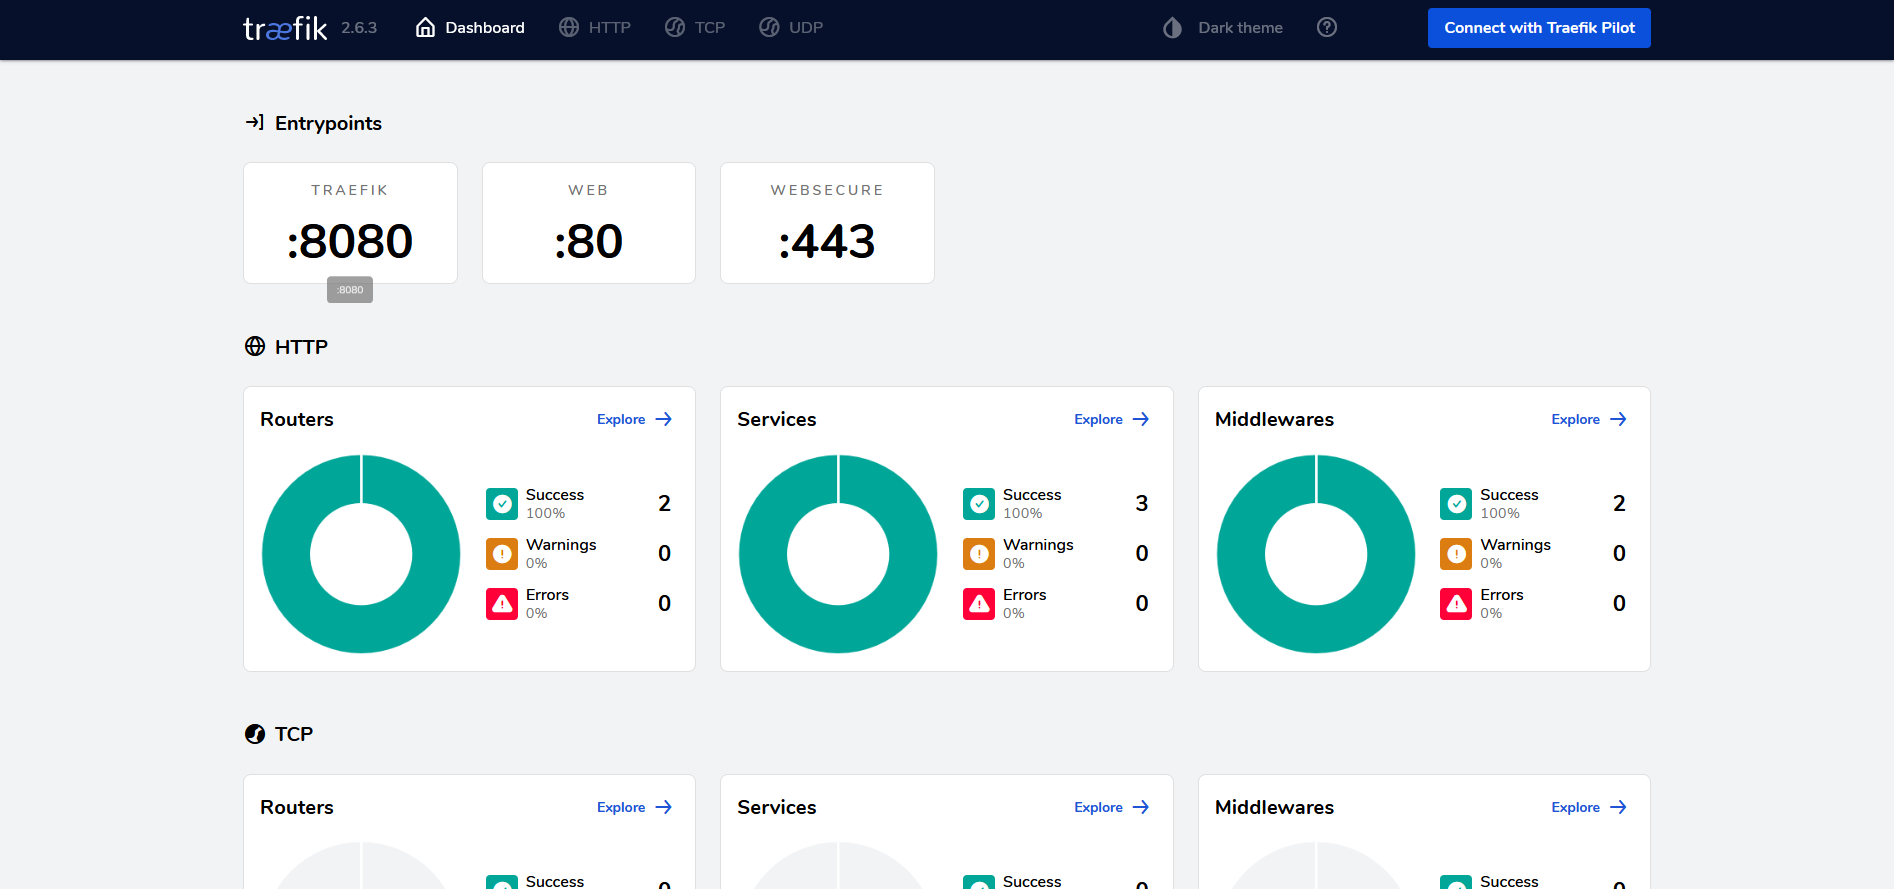
\includegraphics[width=0.8\textwidth]{pics/TreafikDashboard.PNG}
  \centering
  \caption{Dashboard Traefik}
  \label{fig:treafikDashboard}
\end{figure}

\subsection{Dockerfiles}
\subsubsection{Keycloak Docker}
\begin{lstlisting}[caption=Keycloak Dockerfile, label=lst:Dockerfile Keycloak]
version: '3.9'
services:
  keycloak:
  # Name des Containers
    container_name: keycloak
  environment:
    # Zugriffsdaten
      - KEYCLOAK_USER=admin
      - KEYCLOAK_PASSWORD=admin
    # Eingebaute h2 Datenbank
      - DB_VENDOR=h2
    ports:
      - '8180:8080'
    # Image auf dem Aufgebaut wird
    image: 'quay.io/keycloak/keycloak:15.0.2'
    volumes:
    # Speicherort der Zertifikate der Benutzer und Benutzerinnen  
      - ./certs:/etc/ssl/certs/java
    # Speicherort der Keycloak Standarteinstellungen
      - ./imports:/opt/jboss/keycloak/imports
    # Einlesen der Standardeinstellungen und Verhalten des Einlesens bereits vorhandene Objekte nicht ersetzeten
    command: [ '-b', '0.0.0.0', '-Dkeycloak.profile.feature.upload_scripts=enabled', '-Djavax.net.ssl.trustStore=/etc/ssl/certs/java/cacerts', '-Djavax.net.ssl.trustStorePassword=changeit', '-Dkeycloak.migration.action=import', '-Dkeycloak.migration.provider=singleFile','-Dkeycloak.migration.strategy=IGNORE_EXISTING' ,'-Dkeycloak.migration.file=/opt/jboss/keycloak/imports/keycloak_settings.json' ]
    networks:
      - keycloak_network

networks:
  keycloak_network:
    name: keycloak_network
    driver: bridge
\end{lstlisting}
Die importierten Standardeinstellungen erstellen automatisch das Realm, Clients für Frontend und Backend, die Rollen, etc. die 
für die Benutzung gebraucht werden. Somit müssen die Einstellungen nicht jedesmal beim Starten manuell ausgeführt werden.
\begin{lstlisting}[caption=Auszug aus den importieren Einstellungen, label=lst:Imortierte Einstellungen]
  {
    "id": "School",
    "realm": "School",
    "notBefore": 0,
    "defaultSignatureAlgorithm": "RS256",
    "revokeRefreshToken": false,
    "refreshTokenMaxReuse": 0,
    "accessTokenLifespan": 300,
    "accessTokenLifespanForImplicitFlow": 900,
    "ssoSessionIdleTimeout": 1800,
    "ssoSessionMaxLifespan": 36000,
    "ssoSessionIdleTimeoutRememberMe": 0,
    "ssoSessionMaxLifespanRememberMe": 0,
    "offlineSessionIdleTimeout": 2592000,
    "offlineSessionMaxLifespanEnabled": false,
    "offlineSessionMaxLifespan": 5184000,
    "clientSessionIdleTimeout": 0,
    "clientSessionMaxLifespan": 0,
    "clientOfflineSessionIdleTimeout": 0,
    "clientOfflineSessionMaxLifespan": 0,
    "accessCodeLifespan": 60,
    "accessCodeLifespanUserAction": 300,
    ...
\end{lstlisting}

\subsubsection{Postges Docker}
\begin{lstlisting}[caption=Postgres Dockerfile, label=lst:Postges Dockerfile]
  version: '3.1'
  services:
    # Datenbank
    db:
    # Containername
      container_name: survey_postgres
    # Image auf das Aufgebaut wird
      image: postgres:13.3-alpine
  
    # Bei (manuell oder anderweitigen) stoppen der DB wird, nicht neu gestartet wird, selbst wenn der Docker-Daemon neu startet
      restart: unless-stopped
    # Zugriffsdaten
      environment:
        POSTGRES_USER: postgres
        POSTGRES_PASSWORD: postgres
        POSTGRES_DB: db
      ports:
        - 5432:5432
      volumes:
      # Speicherort der permanenten Daten
        - ./db-postgres/db:/var/lib/postgresql/data
      # Importdatenspeicherort
        - ./db-postgres/import:/import
      networks:
        - postgres
  
    # grafische Tool zur Entwicklung und Administration
    pgadmin:
      container_name: survey_pgadmin
      image: dpage/pgadmin4:5.5
      environment:
        PGADMIN_DEFAULT_EMAIL: ${PGADMIN_DEFAULT_EMAIL:-pgadmin4@pgadmin.org}
        PGADMIN_DEFAULT_PASSWORD: ${PGADMIN_DEFAULT_PASSWORD:-admin}
        PGADMIN_CONFIG_SERVER_MODE: 'False'
      volumes:
        - ./db-postgres/pgadmin:/root/.pgadmin
      ports:
        - 8090:80
      networks:
        - postgres
      restart: unless-stopped
  
  networks:
    postgres:
      driver: bridge  
\end{lstlisting}

\subsection{Fragebogen duplizieren}
In dieser Diplomarbeit besteht die Möglichkeit, Fragebögen zu duplizieren. Dies wurde mit dem Code von
\ref{lst:duplicateQuestionnaire} umgesetzt. In diesem Code wird der übergebene Questionnaire ohne id in der Datenbank
gespeichert. Da damit aber nur der Fragebogen und nicht die Fragen oder die Antwortmöglichkeiten dupliziert wurde,
müssen die Questions und AnswerOptions gefunden werden, welche für den aktuellen Fragebogen verwendet werden.
Ist dies geschehen, werden auch diese Daten ohne id in der Datenbank gespeichert. Erst wenn das alles erfüllt ist,
wurde der Fragebogen richtig kopiert.
\begin{lstlisting} [caption=Fragebogen duplizieren, label=lst:duplicateQuestionnaire]
public Questionnaire duplicateQuestionnaire(Questionnaire questionnaire, Interviewer interviewer) {
  Questionnaire originalQuestionnaire = findQuestionnaire(questionnaire);
  Questionnaire duplicateQuestionnaire;
  duplicateQuestionnaire = new Questionnaire(
    originalQuestionnaire.name,
    originalQuestionnaire.description,
    false,
    interviewer);
  duplicateQuestionnaire = save(duplicateQuestionnaire);
  Question duplicateQuestion;
  List<Question> questions = questionRepository.findByQuestionnaire(originalQuestionnaire);
  AnswerOption duplicateAnswerOption;
  List<AnswerOption> answerOptions;
  for (Question originalQuestion : questions) {
    duplicateQuestion = new Question(
      originalQuestion.text,
      originalQuestion.sequenceNumber,
      originalQuestion.questiontype,
      duplicateQuestionnaire);
    duplicateQuestion = questionRepository.save(duplicateQuestion);
    answerOptions = answerOptionRepository.findByQuestionId(originalQuestion.id);
    for (AnswerOption originalAnswerOption : answerOptions) {
      duplicateAnswerOption = new AnswerOption(
        originalAnswerOption.text,
        originalAnswerOption.value,
        originalAnswerOption.sequenceNumber,
        originalAnswerOption.isCorrectAnswer,
        duplicateQuestion);
      duplicateAnswerOption = answerOptionRepository.save(duplicateAnswerOption);
    }
  }
  return duplicateQuestionnaire;
}
\end{lstlisting}

\subsection{Auswertung}
Um herauszufinden, wie die Umfrage ausgefallen ist, gibt es die Auswertung. Bei dieser Diplomarbeit wurde sich dafür
entschieden, zwei verschiedene Arten von Auswertungen zu implementieren:
\begin{enumerate}
  \item Auswertung pro Frage
  \item Auswertung pro Befragten
\end{enumerate}
\subsubsection{Auswertung pro Frage}
Bei der ersten Variante wurde sich dafür entschieden, anzuzeigen, wie oft eine Antwortmöglichkeit
ausgewählt wurde. Wie so eine Auswertung aussehen kann, sieht man in Abbildung\ref{fig:auswertungErgebnis1}.
\newline
\newline
\newline
\begin{figure}[h]
  \centering
    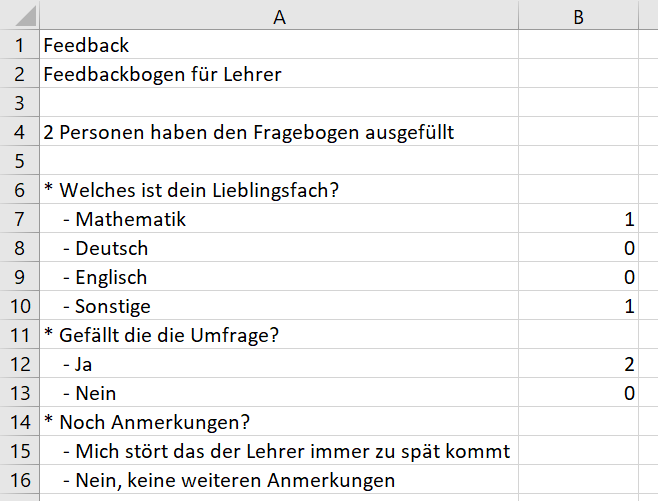
\includegraphics[width=0.5\textwidth]{pics/auswertung1.png}
    \caption{Auswertung}
    \label{fig:auswertungErgebnis1}
\end{figure}

Wie diese Auswertung umgsetzt wurde, wird in \ref{lst:auswertung1} gezeigt.
Mithilfe eines StringBuilders wurden alle nötigen Informationen zu einem String zusammengefügt und danach
mittels PrintWriter in das evaluation.csv File geschrieben. Es werden folgende Daten benötigt:
\begin{itemize}
  \item Name und Beschreibung vom aktuellen Fragebogen
  \item wie viele Transaktionscodes verwendet wurden, mit einem Verweis auf die aktuelle Umfrage
  \item für jede Frage jeweils
  \subitem den Namen
  \subitem die Antwortmöglichkeiten
  \subitem die Anzahl, wie oft eine Antwortmöglichkeit ausgewählt wurde
\end{itemize}
Es wird außerdem überprüft, ob eine Frage vom Typen Freetext ist. Ist dies der Fall, wird die Antwort dieser Frage
am Ende des Files angehängt.
\begin{lstlisting} [caption=Auswertung, label=lst:auswertung1]
  Survey survey = findById(surveyId);
  Questionnaire questionnaire = questionnaireRepository.findById(survey.questionnaire.id);
  List<Question> questions = questionRepository.getQuestionsByQuestionaireId(questionnaire.id);
  List<Transaction> transactions = transactionRepository.findBySurvey(survey);
  for (Transaction transaction : transactions) {
      if (transaction.isUsed){
          usedTransactions ++;
      }
  }
  File file = new File("evaluation.csv");
  try (PrintWriter writer = new PrintWriter("evaluation.csv")) {
      StringBuilder sb = new StringBuilder();
      sb.append(questionnaire.name);
      sb.append(questionnaire.description);
      sb.append(usedTransactions);
      sb.append(" Personen haben den Fragebogen ausgefuellt");
      for (Question question : questions) {
          sb.append(question.text);
          answers = answerRepository.findByQuestion(question);
          if (question.questiontype.equals(QuestionType.FREETEXT)){
              for (Answer answer : answers) {
                  sb.append("    - ");
                  sb.append(answer.answerText);
              }
          }else{
              answerOptions = answerOptionRepository.findByQuestionId(question.id);
              for (AnswerOption answerOption : answerOptions) {
                  chosenOptions = chosenOptionRepository.findByAnswerOption(answerOption);
                  sb.append("    - ");
                  sb.append(answerOption.text);
                  sb.append(": ");
                  sb.append(chosenOptions.size());
              }
          }
      }
      writer.write(sb.toString());
  } catch (FileNotFoundException e) {
      System.out.println(e.getMessage());
  }
\end{lstlisting}
Bei der zweiten Variante wurde sich dafür entschieden, pro Befragten den Wert der ausgewählten Antwortmöglichkeit
anzuzeigen. Wie so eine Auswertung aussehen kann sieht man in Abbildung \ref{fig:auswertungErgebnis2}.
\begin{figure}[h]
  \centering
    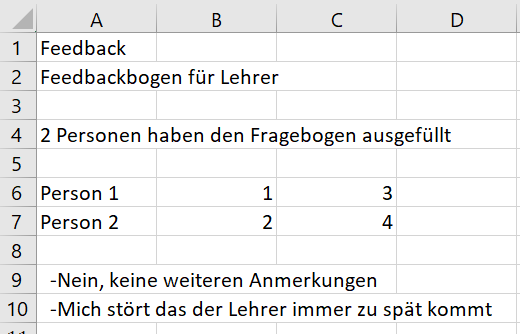
\includegraphics[width=0.5\textwidth]{pics/auswertung2.png}
    \caption{Auswertung}
    \label{fig:auswertungErgebnis2}
\end{figure}

Wie diese Auswertung umgsetzt wurde, wird in \ref{lst:auswertung2} gezeigt.
Mithilfe eines StringBuilders wurden alle nötigen Informationen zu einem String zusammengefügt und danach
mittels PrintWriter in das evaluation2.csv File geschrieben. Es werden folgende Daten benötigt:
\begin{itemize}
  \item Name und Beschreibung vom aktuellen Fragebogen
  \item wie viele Transaktionscodes verwendet wurden, mit einem Verweis auf die aktuelle Umfrage
  \item pro Transaktionscode, der für diese Umfrage verwendet wurde, den Wert der ausgewählten Antwortmöglichkeit, jeder Frage
\end{itemize}
Es wird außerdem überprüft, ob eine Frage vom Typen Freetext ist. Ist dies der Fall, wird die Antwort dieser Frage
am Ende des Files angehängt.
  \begin{lstlisting} [caption=Auswertung, label=lst:auswertung2]
      Survey survey = findById(surveyId);
      Questionnaire questionnaire = questionnaireRepository.findById(survey.questionnaire.id);
      List<Question> questions = questionRepository.getQuestionsByQuestionaireId(questionnaire.id);
      List<Transaction>transactions = transactionRepository.findBySurvey(survey);
      File file = new File("evaluation2.csv");
      try (PrintWriter writer = new PrintWriter("evaluation2.csv")) {
          StringBuilder sb = new StringBuilder();
          sb.append(questionnaire.name);
          sb.append(questionnaire.description);
          sb.append(usedTransactions);
          sb.append(" Personen haben den Fragebogen ausgefuellt");
        
          for (Transaction transaction : transactions) {
              answers = answerRepository.findByTransaction(transaction);
              count ++;
              sb.append("Person ");
              sb.append(count);
              sb.append(";");
              for (Answer answer : answers) {
                  chosenOptions = chosenOptionRepository.findByAnswer(answer);
                  for (ChosenOption chosenOption : chosenOptions) {
                      answerOpt = chosenOption.answerOption;
                      if (chosenOption.question.questiontype == QuestionType.FREETEXT){
                          sb.append("\n");
                          freetextAnswers.add(chosenOption.answer);
                      }else {
                          sb.append(" ");
                          sb.append(answerOpt.value);
                          sb.append(";");
                      }
                  }
              }
          }
          if (freetextAnswers.size() != 0){
              for (Answer answer : freetextAnswers) {
                  sb.append("\n");
                  sb.append("  -");
                  sb.append(answer.answerText);
              }
          }
          writer.write(sb.toString());
      } catch (FileNotFoundException e) {
          System.out.println(e.getMessage());
      }
      return file;
  }
  \end{lstlisting}


\section{Besondere Probleme, die gelöst wurden}
\setauthor{Raffeiner Christine, Weissengruber Nina}
\subsection{Bild speichern im Backend}
Hauptgrund für die schlussendliche Nichtimplementierung des optionalen Speicherns von Bilder zu Fragen war vorallem
die Zeiteinteilung, da das Anliegen für das Einbinden von Bildern erst kurz vor Abgabe der Arbeit aufgekommen ist.
Trotz dessen wurden Versuche für die Speicherung im Backend unternommen. Diese wurden jedoch im weiteren Verlauf
eingestellt.
\newline
\newline
Um ein Bild in der Datenbank zu speichern, kann ein Objekt von Typ byte[] erstellt werden. (Siehe: \ref{lst:lob})
\begin{lstlisting} [caption= @Lob, label=lst:lob]
    @Lob
    @Column(name = "photo")
    private byte[] photo;
\end{lstlisting}
Das übergebene Bild muss in ein byte[] umgewandelt werden, um dieses zu speichern.
Um dies zu erreichen, wurden folgende Versuche unternommen:

\subsubsection{Bild in Byte Array umwandeln}
Beim ersten Versuch wurde das Bild mithilfe eines ImageIO.read() gelesen und mit einem ByteArrayOutputStream
in einem Array gespeichert. Danach wurde das Array durch einen ByteArrayInputStream eingelesen und mit
ImageIO.write() im File output.jpg gespeichert.

\begin{lstlisting} [caption=Bild in Byte Array umwandeln, label=lst:ImageToByteArray]
    public void saveImage(File imageFile){
       BufferedImage bImage = null;
        try {
            bImage = ImageIO.read(imageFile);
        } catch (IOException e) {
            e.printStackTrace();
            System.out.println(e.getMessage());
        }
        ByteArrayOutputStream bos = new ByteArrayOutputStream();
        try {
            ImageIO.write(bImage, "jpg", bos );
        } catch (IOException e) {
            e.printStackTrace();
        }
        byte [] data = bos.toByteArray();
        Question question = new Question("hallo", data, 100, QuestionType.FREETEXT,null);
        save(question);
    }

    public File returnImage(byte[] data){
        ByteArrayInputStream bis = new ByteArrayInputStream(data);
        BufferedImage bImage2 = null;
        try {
            bImage2 = ImageIO.read(bis);
        } catch (IOException e) {
            e.printStackTrace();
        }
        try {
            ImageIO.write(bImage2, "jpg", new File("output.jpg") );
        } catch (IOException e) {
            e.printStackTrace();
        }
        File imageFile = new File("output.png");
        return imageFile;
    }
\end{lstlisting}

\subsubsection{Bild mit Session in DB speichern}
Beim zweiten Versuch wurde mithilfe von HibernateUtil.getSessionFactory().openSession() eine Session eröffnet,
in der mittels eine FileInputStream das Bild in ein byte[] ungewandelt wird. Danach wird das erzeugte byte[] 
in der DB gespeichert. Um das byte[] aus der DB zu laden und in ein File umzuwandeln, verwendet man den
FileOutputStream.
\newline
\newline
Dieser Versuch wurde anfangs mit einem Bild, das lokal auf dem Rechner liegt, getestet. Dabei wurde das Bild
in der DB gespeichert und wieder geladen. Als ausporbiert wurde, ob dieser Versuch funktioniert, wenn das Bild
vom Frontend mitgesendet wird, trat der Fehler auf, dass man ein mitgeschicktes File nicht so leicht umwandeln kann.
Nach dieser Erkenntnis wurde auch dieser Versuch eingestellt.

\begin{lstlisting} [caption=Bild mit Session in DB speichern, label=lst:imageSessionSave]
public static void main( String[] args )
    {
        System.out.println("Hibernate save image into database");
        Session session = HibernateUtil.getSessionFactory().openSession();
        
        session.beginTransaction();
        
        //save image into database
        File file = new File("C:\\mavan-hibernate-image-mysql.gif");
        byte[] bFile = new byte[(int) file.length()];
        
        try {
         FileInputStream fileInputStream = new FileInputStream(file);
         //convert file into array of bytes
         fileInputStream.read(bFile);
         fileInputStream.close();
        } catch (Exception e) {
         e.printStackTrace();
        }
        
        Avatar avatar = new Avatar();
        avatar.setImage(bFile);
        
        session.save(avatar);
        
        //Get image from database
        Avatar avatar2 = (Avatar)session.get(Avatar.class, avatar.getAvatarId());
        byte[] bAvatar = avatar2.getImage();
        
        try{
            FileOutputStream fos = new FileOutputStream("C:\\test.gif"); 
            fos.write(bAvatar);
            fos.close();
        }catch(Exception e){
            e.printStackTrace();
        }

        session.getTransaction().commit();
    }
\end{lstlisting}

\subsection{CORS Fehler}
Nach der Implementierung einiger Hauptfunktionen im Frontend -- zum Beispiel das Erstellen eines Fragebogen --
wurden diese mit den bereits erstellten REST-Methoden verbunden und getestet. Im Laufe der Testungen sind 
CORS Fehler aufgetreten. Wie so ein Fehler aussieht wird beispielhaft in Abb. \ref{fig:cors} dargestellt.
Ein CORS Fehler entsteht beim Laden von Daten aus verschiedenen Quellen. Das Problem wurde durch das Einfügen 
von folgender Zeile \ref{lst:CorsError} in den application.properties behoben.

\begin{figure}[H]
    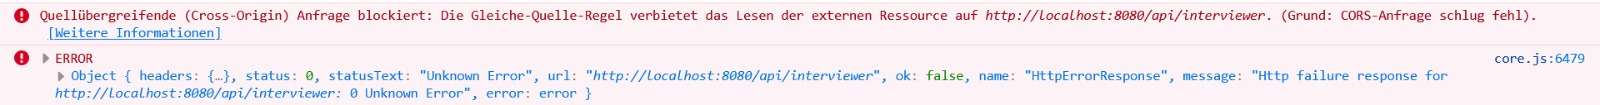
\includegraphics[width=1\textwidth]{pics/cors_error.jpeg}
    \centering
    \caption{CORS Fehler}
    \label{fig:cors}
\end{figure}

\begin{lstlisting} [caption=Lösung CORS Error, label=lst:CorsError]
    quarkus.http.cors=true
\end{lstlisting}

\subsection{Cyclic-Object-Error}
Cyclic-Object-Error (siehe Abb. \ref{fig:cycle} als Beispiel) können bei der Konvertierung von Angular-Objekten in 
JSON-Objekte auftreten. \cite{noauthor_typeerror_nodate}, \cite{noauthor_fixing_nodate}

Der Fehler tritt genau dann auf wenn:
\begin{enumerate}
    \item ein Objekt auf sich selbst referenziert
    \item zwei Objekte aufeinander referenzieren
    \item mehreren Objekten, die in einen Kreis aufeinander referenzieren, konvertiert werden sollen
\end{enumerate}

Das JSON-Format an sich unterstützt keine Objektreferenzen, daher versucht JSON.stringify() nicht, diese zu lösen, und schlägt entsprechend fehl. 
Veranschaulicht würde das JSON-Objekte unendlich lang und in die Tiefe gehen.
\begin{figure}[H]
  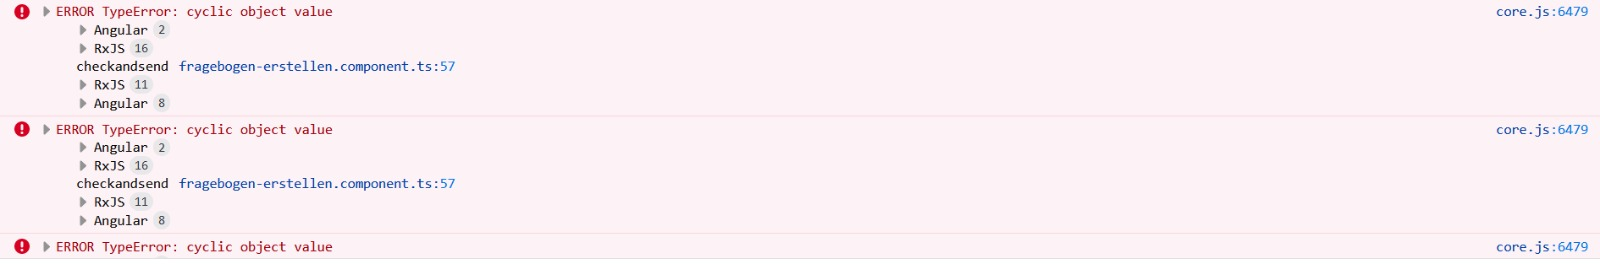
\includegraphics[width=1.2\textwidth]{pics/cycle_object.jpeg}
  \centering
  \caption{Cyclic-Object-Error}
  \label{fig:cycle}
\end{figure}
In der vorliegenden Arbeit wurde versehentlich ein Cyclic-Object erstellt, um die Darstellung von Fragen und zugehörigen
Antwortmöglichkeiten zu gewährleisten. Dabei referenzierte die Frage auf die Antwortmöglichkeit und die Antwortmöglichkeit auf die Frage.
Die Referenzierung der Antwortmöglichkeiten auf die Frage ist durch das Backend vorgegeben worden. Die Referenzierung der Antwortmöglichkeit auf die Frage 
wurde für die einfachere Zuordnung und Darstellung der beiden im Frontend eingefügt. (siehe Listing \ref{lst:alte Klassen mit cycle-error})
\begin{lstlisting}[language=TypeScript, caption=Klassen mit Cyclic-Error, label=lst:alte Klassen mit cycle-error]
import { Interviewer } from "./interviewer";
import { AnswerOption } from "./answer-option"

export class Questionnaire {
  constructor(
    public id = 0, public name :string = "", 
    public description : string = "", 
    public isPublic: Boolean = false, 
    public interviewer : Interviewer = new Interviewer(1, "HTL Leonding"),
    public AnswerOptions : AnswerOption[] = []
    ){}
}

import { Question } from "./question";

export class AnswerOption {
    constructor(
      public id = 0, public text :string = "", 
      public value = 0, 
      public sequenceNumber = 0, 
      public isCorrectAnswer = true, 
      public question : Question = new Question()
    ){}
}
\end{lstlisting}
Für die Übertragung von Daten zwischen Frontend und Backend wurde beschlossen JSON zu verwenden.
Dieses Format kann diese Referenzierung nicht darstellen und die einmalige Verwendung von
cycle.js, einer Bibliothek, die solche Referenzierung darstellen kann, wäre zu aufwändig gewesen.
\newline
\newline
Für die Lösung dieses Problem wurde eine neue Klasse erstellt und beide Objekte (Frage und Antwortmöglichkeiten-Liste) 
einander zugeordnet. Somit konnte die Referenzierung der Antwortmöglichkeit auf die Frage entfernt und der 
Cyclic-Object-Error gelöst werden.
\begin{lstlisting}[language=TypeScript, caption=Klassen ohne Cyclic-Error, label=lst:neue Klassen ohne cycle-error]
  import { AnswerOption } from "./answer-option"
  import { Question } from "./question"
  
  export class Administration {
      constructor(
        public question : Question = new Question(), 
        public answerOptionArray : Array<AnswerOption>, 
        public aocounter = 1
      ){}
  }  
\end{lstlisting}

\setauthor{Raffeiner Christine}
\section{Entwurfsentscheidungen}
\subsection{Verwendung von CSS, SCSS, SASS oder Less}
Die Entscheidung welches Stylesheet zur Layoutierung von Angular verwendet wird, war von Anfang an klar.
Technologien wie SASS und Less (siehe Kapitel \ref{chap:stylesheet}) kamen nicht in Frage, da dem Team diese Technologien eher unbekannt sind.
Übrig blieben folgend CSS und SCSS. Die Entscheidung wurde für SCSS getroffen, da es 
eine Obermenge von CSS mit mehr Funktionen ist.

\subsection{Entscheidung zwischen Angular und anderen Frameworks}
\setauthor{Raffeiner Christine}
Nicht nur wird Angular von vielen Unternehmen für ihre Projekte verwendet, sondern liefert es auch im Gegensatz zu anderen Frameworks 
eine vorgegeben Struktur, die die Verwendung erleichtern. Auch bietet Angular die benötigte Leistungsfähigkeit für die Erstellung des Frontends. 
Die Entscheidung wurde zudem durch längere Erfahrung mit dem Framework Angular und Mangel an Erfahrung mit anderen Frameworks 
wie React oder Vue verstärkt. \cite{noauthor_angular_nodate-5}, \cite{noauthor_angular_nodate-6}, \cite{noauthor_vue_nodate}

\setauthor{Weissengruber Nina}
\subsection{Entscheidung Java}
Wir haben uns einerseits für diese Programmiersprache entschieden, 
einerseits da sie uns seit der ersten Klasse an der HTL Leonding beigebracht wird und wir dadurch gewisse 
Grundkenntnisse in Java besitzen. Andererseits, da unser Diplomarbeitsbetreuer sehr gute Kenntnisse in Java 
besitzt und wir bei Fragen uns an ihn wenden können. Weiteres existiert im Internet eine große Community, 
die Hilfestellungen oder Problemlösungen dokumentiert und bereitstellt.

\subsection{Entscheidung PostgreSql}
Wir haben uns für PostgreSql entschieden, da PostgreSql dem SQL-Standard entspricht. 
Außerdem ist PostgreSql nicht an ein Betriebssystem gebunden.


\begin{spacing}{1}
\chapter{Implementierung}
\end{spacing}
\setauthor{Weissengruber Nina}
\section{Endpoints}
\subsection{Transaction}
\subsubsection{find all}
\textbf{GET} \emph{https://localhost:8080/api/transaction}

\textbf{Rückgabewert}
Zurückgegeben wird eine Liste von allen Transactionen als JSON
Format.

\subsubsection{find By Id}
\textbf{GET} \emph{https://localhost:8080/api/transaction/id/\{id\}}

\textbf{Parameter}
\begin{itemize}
    \item \emph{id}: eindeutige Nummer einer Transaction
\end{itemize}

\textbf{Rückgabewert}
Zurückgegeben wird das gefundene Transaction Objekt als JSON Format. Wenn keines mit der angegeben \emph{id} gefunden wird, so wird der
HTTP Error \emph{No Content (204)} zurückgegeben.

\subsubsection{create Transaction}
\textbf{POST} \emph{https://localhost:8080/api/transaction}

\textbf{Body}
\begin{itemize}
    \item Transaction Objekt im JSON Format
    \item UriInfo
\end{itemize}

\textbf{Aktion}
In der Datenbank wird das übergebene Transaction Objekt persistiert.

\textbf{Rückgabewert}
Zurückgegeben wird die URI, über welche das soeben erstellte Objekt über einen anderen Endpoint angefordert werden kann.

\subsubsection{get Transaction with code}
\textbf{GET} \emph{https://localhost:8080/api/transaction/code/\{code\}}

\textbf{Parameter}
\begin{itemize}
    \item \emph{code}: String mit dem Code einer Transaction
\end{itemize}

\textbf{Rückgabewert}
Zurückgegeben wird das gefundene Transaction Objekt als JSON Format. Wenn keines mit der angegeben \emph{id} gefunden wird, so wird der
HTTP Error \emph{No Content (204)} zurückgegeben.

\subsubsection{get Survey with Transaction}
\textbf{POST} \emph{https://localhost:8080/api/transaction/getSurvey}

\textbf{Body}
\begin{itemize}
    \item Transaction Objekt im JSON Format
\end{itemize}

\textbf{Aktion}
Es werden alle Survey Objekte mit einer referenz auf das übergebene Transaction Objekt gesucht.

\textbf{Rückgabewert}
Zurückgegeben wird eine Liste von Survey Objekten.

\subsubsection{update Transaction}
\textbf{POST} \emph{https://localhost:8080/api/transaction/\{id\}}

\textbf{Body}
\begin{itemize}
    \item id: eindeutige Nummer einer Transaction
    \item Transaction Objekt im JSON Format
\end{itemize}

\textbf{Aktion}
In der Datenbank wird das wird das bereits persistierte Objekt aktualisiert.

\textbf{Rückgabewert}
Zurückgegeben wird das persistierte Objekt. Wenn keines mit der angegeben id gefunden wird, so wird der HTTP Error Bad Request
(400) zurückgegeben.

\subsubsection{delete Transaction}
\textbf{DELETE} \emph{https://localhost:8080/api/transaction/\{id\}}

\textbf{Body}
\begin{itemize}
    \item id: eindeutige Nummer einer Transaction
\end{itemize}

\textbf{Aktion}
Es wird das Transaction Objekt mit der übergebenen Id gesucht und anschließend
aus der Datenbank gelöscht.

\textbf{Rückgabewert}
Nach einem erfolgreichen lösch Vorgang wird der http status \emph{ok (200)} zurückgegeben.

\subsubsection{generate Transaction}
\textbf{GET} \emph{https://localhost:8080/api/transaction/generate/\{number\}/\{surveyId\}}

\textbf{Parameter}
\begin{itemize}
    \item \emph{surveyId}: eindeutige Nummer einer Survey
    \item \emph{number}: Anzahl wie viele Transactions generiert werdern müssen
\end{itemize}

\textbf{Aktion}
Es wird die Anzahl der gewünschten Transactions erstellt und in der Datenbank persistiert 

\textbf{Rückgabewert}
Zurückgegeben wird ein File in dem alle Codes der neu generierten Transactions stehen.

\subsection{Survey}
\subsubsection{find All}
\textbf{GET} \emph{https://localhost:8080/api/survey}

\textbf{Rückgabewert}
Zurückgegeben wird eine Liste von allen Survey Objekten als JSON
Format.

\subsubsection{find By Id}
\textbf{GET} \emph{https://localhost:8080/api/survey/id/\{id\}}

\textbf{Parameter}
\begin{itemize}
    \item \emph{id}: eindeutige Nummer einer Survey
\end{itemize}

\textbf{Rückgabewert}
Zurückgegeben wird das gefundene Survey Objekt als JSON Format. Wenn keines mit der angegeben \emph{id} gefunden wird, so wird der
HTTP Error \emph{No Content (204)} zurückgegeben.


\subsubsection{create Survey}
\textbf{POST} \emph{https://localhost:8080/api/survey}

\textbf{Body}
\begin{itemize}
    \item Survey Objekt im JSON Format
    \item UriInfo
\end{itemize}

\textbf{Aktion}
In der Datenbank wird das übergebene Survey Objekt persistiert.

\textbf{Rückgabewert}
Zurückgegeben wird die URI, über welche das soeben erstellte Objekt über einen anderen Endpoint angefordert werden kann.

\subsubsection{find Survey by Interviewer Id}
\textbf{GET} \emph{https://localhost:8080/api/survey/\{interviewerId\}}

\textbf{Parameter}
\begin{itemize}
    \item \emph{interviewerId}: eindeutige Nummer eines Interviewers
\end{itemize}

\textbf{Rückgabewert}
Zurückgegeben wird das gefundene Survey Objekt als JSON Format. 

\subsubsection{find Questionnaire with Survey Id}
\textbf{GET} \emph{https://localhost:8080/api/survey/questionnaire/\{surveyId\}}

\textbf{Parameter}
\begin{itemize}
    \item \emph{surveyId}: eindeutige Nummer einer Survey
\end{itemize}

\textbf{Rückgabewert}
Zurückgegeben wird das gefundene Questionnaire Objekt als JSON Format.

\subsubsection{update Survey}
\textbf{POST} \emph{https://localhost:8080/api/survey/\{id\}}

\textbf{Body}
\begin{itemize}
    \item id: eindeutige Nummer einer Survey
    \item Survey Objekt im JSON Format
\end{itemize}

\textbf{Aktion}
In der Datenbank wird das wird das bereits persistierte Objekt aktualisiert.

\textbf{Rückgabewert}
Zurückgegeben wird das persistierte Objekt. Wenn keines mit der angegeben id gefunden wird, so wird der HTTP Error Bad Request
(400) zurückgegeben.

\subsubsection{delete Survey}
\textbf{DELETE} \emph{https://localhost:8080/api/survey/\{id\}}

\textbf{Body}
\begin{itemize}
    \item id: eindeutige Nummer einer Survey
\end{itemize}

\textbf{Aktion}
Es wird das Survey Objekt mit der übergebenen Id gesucht und anschließend
aus der Datenbank gelöscht.

\textbf{Rückgabewert}
Nach einem erfolgreichen lösch Vorgang wird der http status \emph{ok (200)} zurückgegeben.

\subsubsection{Auswertung}
\textbf{GET} \emph{https://localhost:8080/api/survey/evaluation/\{surveyId\}}

\textbf{Parameter}
\begin{itemize}
    \item \emph{surveyId}: eindeutige Nummer einer Survey
\end{itemize}

\textbf{Rückgabewert}
Zurückgegeben wird ein File mit der Auswertung.

\subsection{Question}
\subsubsection{find All}
\textbf{GET} \emph{https://localhost:8080/api/question}

\textbf{Rückgabewert}
Zurückgegeben wird eine Liste von allen Question Objekten als JSON
Format.

\subsubsection{find By Id}
\textbf{GET} \emph{https://localhost:8080/api/question/id/\{id\}}

\textbf{Parameter}
\begin{itemize}
    \item \emph{id}: eindeutige Nummer einer Question
\end{itemize}

\textbf{Rückgabewert}
Zurückgegeben wird das gefundene Question Objekt als JSON Format. Wenn keines mit der angegeben \emph{id} gefunden wird, so wird der
HTTP Error \emph{No Content (204)} zurückgegeben.

\subsubsection{create Question}
\textbf{POST} \emph{https://localhost:8080/api/question}

\textbf{Body}
\begin{itemize}
    \item Question Objekt im JSON Format
    \item UriInfo
\end{itemize}

\textbf{Aktion}
In der Datenbank wird das übergebene Question Objekt persistiert.

\textbf{Rückgabewert}
Zurückgegeben wird die URI, über welche das soeben erstellte Objekt über einen anderen Endpoint angefordert werden kann.

\subsubsection{update Question}
\textbf{POST} \emph{https://localhost:8080/api/question/\{id\}}

\textbf{Body}
\begin{itemize}
    \item id: eindeutige Nummer einer Question
    \item Question Objekt im JSON Format
\end{itemize}

\textbf{Aktion}
In der Datenbank wird das wird das bereits persistierte Objekt aktualisiert.

\textbf{Rückgabewert}
Zurückgegeben wird das persistierte Objekt. Wenn keines mit der angegeben id gefunden wird, so wird der HTTP Error Bad Request
(400) zurückgegeben.

\subsubsection{delete Question}
\textbf{DELETE} \emph{https://localhost:8080/api/question/\{id\}}

\textbf{Body}
\begin{itemize}
    \item id: eindeutige Nummer einer Question
\end{itemize}

\textbf{Aktion}
Es wird das Question Objekt mit der übergebenen Id gesucht und anschließend
aus der Datenbank gelöscht.

\textbf{Rückgabewert}
Nach einem erfolgreichen lösch Vorgang wird der http status \emph{ok (200)} zurückgegeben.

\subsection{Questionnaire}
\subsubsection{find All}
\textbf{GET} \emph{https://localhost:8080/api/questionnaire}

\textbf{Rückgabewert}
Zurückgegeben wird eine Liste von allen Questionnaire Objekten als JSON
Format.

\subsubsection{find By Id}
\textbf{GET} \emph{https://localhost:8080/api/questionnaire/id/\{id\}}

\textbf{Parameter}
\begin{itemize}
    \item \emph{id}: eindeutige Nummer einer Questionnaire
\end{itemize}

\textbf{Rückgabewert}
Zurückgegeben wird das gefundene Questionnaire Objekt als JSON Format. Wenn keines mit der angegeben \emph{id} gefunden wird, so wird der
HTTP Error \emph{No Content (204)} zurückgegeben.

\subsubsection{create Questionnaire}
\textbf{POST} \emph{https://localhost:8080/api/questionnaire}

\textbf{Body}
\begin{itemize}
    \item Questionnaire Objekt im JSON Format
    \item UriInfo
\end{itemize}

\textbf{Aktion}
In der Datenbank wird das übergebene Questionnaire Objekt persistiert.

\textbf{Rückgabewert}
Zurückgegeben wird die URI, über welche das soeben erstellte Objekt über einen anderen Endpoint angefordert werden kann.

\subsubsection{find public Questionnaires}
\textbf{GET} \emph{https://localhost:8080/api/questionnaire/public}

\textbf{Rückgabewert}
Zurückgegeben wird eine Liste von Questionnaire Objekten, bei denen das Attribut isPublic auf true gestezt ist.

\subsubsection{get public and owned Questionnaires}
\textbf{GET} \emph{https://localhost:8080/api/questionnaire/public/\{interviewerId\}}

\textbf{Body}
\begin{itemize}
    \item interviewerId: eindeutige Nummer eines Interviewers
\end{itemize}

\textbf{Rückgabewert}
Zurückgegeben wird eine Liste von Questionnaire Objekten, bei denen das Attribut isPublic auf true gestezt ist 
und eine referenz auf das übergebene Interviewer Onjekt besteht.

\subsubsection{find Questionnaire By Interviwer id}
\textbf{GET} \emph{https://localhost:8080/api/questionnaire/interviwer/\{interviewerId\}}

\textbf{Body}
\begin{itemize}
    \item interviewerId: eindeutige Nummer eines Interviewers
\end{itemize}

\textbf{Rückgabewert}
Zurückgegeben wird eine Liste von Questionnaire Objekten, bei denen 
eine referenz auf das übergebene Interviewer Onjekt besteht.

\subsubsection{duplicate Questionnaire}
\textbf{POST} \emph{https://localhost:8080/api/duplicateQuestionnaire}

\textbf{Body}
\begin{itemize}
    \item Questionnaire Objekt im JSON Format
\end{itemize}

\textbf{Aktion}
Es wird ein duplicat des übergebenen Questionnaire Objekts in der Datenbank persistiert.

\textbf{Rückgabewert}
Zurückgegeben wird das duplizierte Questionnaire Objekt.

\subsubsection{update Questionnaire}
\textbf{POST} \emph{https://localhost:8080/api/questionnaire/\{id\}}

\textbf{Body}
\begin{itemize}
    \item id: eindeutige Nummer einer Questionnaire
    \item Questionnaire Objekt im JSON Format
\end{itemize}

\textbf{Aktion}
In der Datenbank wird das wird das bereits persistierte Objekt aktualisiert.

\textbf{Rückgabewert}
Zurückgegeben wird das persistierte Objekt. Wenn keines mit der angegeben id gefunden wird, so wird der HTTP Error Bad Request
(400) zurückgegeben.

\subsubsection{delete Questionnaire}
\textbf{DELETE} \emph{https://localhost:8080/api/questionnaire/\{id\}}

\textbf{Body}
\begin{itemize}
    \item id: eindeutige Nummer eines Questionnaire
\end{itemize}

\textbf{Aktion}
Es wird das Questionnaire Objekt mit der übergebenen Id gesucht und anschließend
aus der Datenbank gelöscht.

\textbf{Rückgabewert}
Nach einem erfolgreichen lösch Vorgang wird der http status \emph{ok (200)} zurückgegeben.

\subsection{Interviewer}
\subsubsection{find All}
\textbf{GET} \emph{https://localhost:8080/api/interviewer}

\textbf{Rückgabewert}
Zurückgegeben wird eine Liste von allen Interviewer Objekten als JSON
Format.

\subsubsection{find By Id}
\textbf{GET} \emph{https://localhost:8080/api/interviewer/id/\{id\}}

\textbf{Parameter}
\begin{itemize}
    \item \emph{id}: eindeutige Nummer eines Interviewers
\end{itemize}

\textbf{Rückgabewert}
Zurückgegeben wird das gefundene Interviewer Objekt als JSON Format. Wenn keines mit der angegeben \emph{id} gefunden wird, so wird der
HTTP Error \emph{No Content (204)} zurückgegeben.

\subsubsection{create Question}
\textbf{POST} \emph{https://localhost:8080/api/interviewer}

\textbf{Body}
\begin{itemize}
    \item Interviewer Objekt im JSON Format
    \item UriInfo
\end{itemize}

\textbf{Aktion}
In der Datenbank wird das übergebene Interviewer Objekt persistiert.

\textbf{Rückgabewert}
Zurückgegeben wird die URI, über welche das soeben erstellte Objekt über einen anderen Endpoint angefordert werden kann.

\subsubsection{update Interviewer}
\textbf{POST} \emph{https://localhost:8080/api/interviewer/\{id\}}

\textbf{Body}
\begin{itemize}
    \item id: eindeutige Nummer einer Interviewer
    \item Interviewer Objekt im JSON Format
\end{itemize}

\textbf{Aktion}
In der Datenbank wird das wird das bereits persistierte Objekt aktualisiert.

\textbf{Rückgabewert}
Zurückgegeben wird das persistierte Objekt. Wenn keines mit der angegeben id gefunden wird, so wird der HTTP Error Bad Request
(400) zurückgegeben.

\subsubsection{delete Interviewer}
\textbf{DELETE} \emph{https://localhost:8080/api/interviewer/\{id\}}

\textbf{Body}
\begin{itemize}
    \item id: eindeutige Nummer einer Interviewer
\end{itemize}

\textbf{Aktion}
Es wird das Interviewer Objekt mit der übergebenen Id gesucht und anschließend
aus der Datenbank gelöscht.

\textbf{Rückgabewert}
Nach einem erfolgreichen lösch Vorgang wird der http status \emph{ok (200)} zurückgegeben.

\subsection{ChosenOption}
\subsubsection{find All}
\textbf{GET} \emph{https://localhost:8080/api/chosenOption}

\textbf{Rückgabewert}
Zurückgegeben wird eine Liste von allen ChosenOption Objekten als JSON
Format.

\subsubsection{find By Id}
\textbf{GET} \emph{https://localhost:8080/api/chosenOption/id/\{id\}}

\textbf{Parameter}
\begin{itemize}
    \item \emph{id}: eindeutige Nummer einer ChosenOption
\end{itemize}

\textbf{Rückgabewert}
Zurückgegeben wird das gefundene ChosenOption Objekt als JSON Format. Wenn keines mit der angegeben \emph{id} gefunden wird, so wird der
HTTP Error \emph{No Content (204)} zurückgegeben.

\subsubsection{create ChosenOption}
\textbf{POST} \emph{https://localhost:8080/api/chosenOption}

\textbf{Body}
\begin{itemize}
    \item ChosenOption Objekt im JSON Format
    \item UriInfo
\end{itemize}

\textbf{Aktion}
In der Datenbank wird das übergebene ChosenOption Objekt persistiert.

\textbf{Rückgabewert}
Zurückgegeben wird die URI, über welche das soeben erstellte Objekt über einen anderen Endpoint angefordert werden kann.

\subsubsection{update ChosenOption}
\textbf{POST} \emph{https://localhost:8080/api/chosenOption/\{id\}}

\textbf{Body}
\begin{itemize}
    \item id: eindeutige Nummer einer ChosenOption
    \item ChosenOption Objekt im JSON Format
\end{itemize}

\textbf{Aktion}
In der Datenbank wird das wird das bereits persistierte Objekt aktualisiert.

\textbf{Rückgabewert}
Zurückgegeben wird das persistierte Objekt. Wenn keines mit der angegeben id gefunden wird, so wird der HTTP Error Bad Request
(400) zurückgegeben.

\subsubsection{delete ChosenOption}
\textbf{DELETE} \emph{https://localhost:8080/api/chosenOption/\{id\}}

\textbf{Body}
\begin{itemize}
    \item id: eindeutige Nummer einer ChosenOption
\end{itemize}

\textbf{Aktion}
Es wird das ChosenOption Objekt mit der übergebenen Id gesucht und anschließend
aus der Datenbank gelöscht.

\textbf{Rückgabewert}
Nach einem erfolgreichen lösch Vorgang wird der http status \emph{ok (200)} zurückgegeben.

\subsection{Answer}
\subsubsection{find All}
\textbf{GET} \emph{https://localhost:8080/api/answer}

\textbf{Rückgabewert}
Zurückgegeben wird eine Liste von allen Answer Objekten als JSON
Format.

\subsubsection{find By Id}
\textbf{GET} \emph{https://localhost:8080/api/answer/id/\{id\}}

\textbf{Parameter}
\begin{itemize}
    \item \emph{id}: eindeutige Nummer einer Answer
\end{itemize}

\textbf{Rückgabewert}
Zurückgegeben wird das gefundene Answer Objekt als JSON Format. Wenn keines mit der angegeben \emph{id} gefunden wird, so wird der
HTTP Error \emph{No Content (204)} zurückgegeben.

\subsubsection{create Answer}
\textbf{POST} \emph{https://localhost:8080/api/answer}

\textbf{Body}
\begin{itemize}
    \item Answer Objekt im JSON Format
    \item UriInfo
\end{itemize}

\textbf{Aktion}
In der Datenbank wird das übergebene Answer Objekt persistiert.

\textbf{Rückgabewert}
Zurückgegeben wird die URI, über welche das soeben erstellte Objekt über einen anderen Endpoint angefordert werden kann.

\subsubsection{update Answer}
\textbf{POST} \emph{https://localhost:8080/api/answer/\{id\}}

\textbf{Body}
\begin{itemize}
    \item id: eindeutige Nummer einer Answer
    \item Answer Objekt im JSON Format
\end{itemize}

\textbf{Aktion}
In der Datenbank wird das wird das bereits persistierte Objekt aktualisiert.

\textbf{Rückgabewert}
Zurückgegeben wird das persistierte Objekt. Wenn keines mit der angegeben id gefunden wird, so wird der HTTP Error Bad Request
(400) zurückgegeben.

\subsubsection{delete Answer}
\textbf{DELETE} \emph{https://localhost:8080/api/answer/\{id\}}

\textbf{Body}
\begin{itemize}
    \item id: eindeutige Nummer einer Answer
\end{itemize}

\textbf{Aktion}
Es wird das Answer Objekt mit der übergebenen Id gesucht und anschließend
aus der Datenbank gelöscht.

\textbf{Rückgabewert}
Nach einem erfolgreichen lösch Vorgang wird der http status \emph{ok (200)} zurückgegeben.

\subsection{AnswerOption}
\subsubsection{find All}
\textbf{GET} \emph{https://localhost:8080/api/answerOption}

\textbf{Rückgabewert}
Zurückgegeben wird eine Liste von allen AnswerOption Objekten als JSON
Format.

\subsubsection{find By Id}
\textbf{GET} \emph{https://localhost:8080/api/answerOption/id/\{id\}}

\textbf{Parameter}
\begin{itemize}
    \item \emph{id}: eindeutige Nummer einer AnswerOption
\end{itemize}

\textbf{Rückgabewert}
Zurückgegeben wird das gefundene AnswerOption Objekt als JSON Format. Wenn keines mit der angegeben \emph{id} gefunden wird, so wird der
HTTP Error \emph{No Content (204)} zurückgegeben.

\subsubsection{create Answer}
\textbf{POST} \emph{https://localhost:8080/api/answerOption}

\textbf{Body}
\begin{itemize}
    \item AnswerOption Objekt im JSON Format
    \item UriInfo
\end{itemize}

\textbf{Aktion}
In der Datenbank wird das übergebene AnswerOption Objekt persistiert.

\textbf{Rückgabewert}
Zurückgegeben wird die URI, über welche das soeben erstellte Objekt über einen anderen Endpoint angefordert werden kann.

\subsubsection{update AnswerOption}
\textbf{POST} \emph{https://localhost:8080/api/answerOption/\{id\}}

\textbf{Body}
\begin{itemize}
    \item id: eindeutige Nummer einer AnswerOption
    \item AnswerOption Objekt im JSON Format
\end{itemize}

\textbf{Aktion}
In der Datenbank wird das wird das bereits persistierte Objekt aktualisiert.

\textbf{Rückgabewert}
Zurückgegeben wird das persistierte Objekt. Wenn keines mit der angegeben id gefunden wird, so wird der HTTP Error Bad Request
(400) zurückgegeben.

\subsubsection{delete AnswerOption}
\textbf{DELETE} \emph{https://localhost:8080/api/answerOption/\{id\}}

\textbf{Body}
\begin{itemize}
    \item id: eindeutige Nummer einer AnswerOption
\end{itemize}

\textbf{Aktion}
Es wird das AnswerOption Objekt mit der übergebenen Id gesucht und anschließend
aus der Datenbank gelöscht.

\textbf{Rückgabewert}
Nach einem erfolgreichen lösch Vorgang wird der http status \emph{ok (200)} zurückgegeben.



\begin{spacing}{1}
\chapter{Projektorganisation}
\end{spacing}
\section{Anforderungen}
Um die vorliegende Arbeit bestmöglich und ohne größere projektorganisatorische Probleme bewältigen zu können, mussten Hilfsmittel 
gefunden werden, die die folgenden Anforderungen erfüllen können.   
\begin{itemize}
    \item Gemeinsame Codebasis
    \item Versionierung
    \item Visualisierung Arbeitsfortschritt
    \item Arbeitszuteilung
    \item Zu erledigende Aufgaben
\end{itemize}

\section{Mögliche Hilfsmittel}
\subsection{GitHub}
\label{chap:github}
\setauthor{Raffeiner Christine}
GitHub ist eine webbasierte Versionskontroll- und Kollaborationsplattform für Softwareentwickler. 
GitHub wird verwendet, um den Code für ein Projekt zu speichern und den kompletten Verlauf aller 
Änderungen an diesem Code zu verfolgen. Es ermöglicht Entwicklern eine reibungslose Zusammenarbeit 
an einem Projekt, indem es Werkzeuge für die Verwaltung möglicherweise widersprüchlicher Änderungen 
von mehreren Entwicklern bereitstellt. \cite{noauthor_github_2022}

\subsection{GitHub Desktop}
\label{chap:desktop}
GitHub Desktop ist eine Anwendung, die es ermöglicht, 
mit GitHub über eine grafische Benutzeroberfläche zu interagieren, statt über die 
Eingabeaufforderung oder einen Webbrowser. Wie in anderen GitHub-Anbindungen zeigt der GitHub Desktop 
Änderungen aller Art (Löschen, Hinzugefügt und Geändert) grafisch an und ermöglicht die Interaktion mit 
einfachen Klicks. \cite{noauthor_github_nodate}

\subsection{GitHub Projektboards und Issues}
Projektboards auf GitHub helfen die Arbeit zu organisieren und zu priorisieren. 
Projektboards können für die Arbeit an bestimmten Funktionen, umfassende Roadmaps oder sogar zur Erstellung von
Release-Checklisten verwendet werden. Projektboards bieten die Flexibilität, individuelle 
Arbeitsabläufe zu erstellen, die den Bedürfnissen angepasst werden können. Projektboards bestehen aus 
Issues, Pull-Requests und Notizen, die als Cards in Spalten kategorisiert werden. GitHub bietet
die Möglichkeit Meilensteine anzulegen und 1 oder mehrere Issues mit dem Meilenstein zu verlinken. \cite{noauthor_github_nodate-1}

\subsection{YouTrack}
\label{chap:youtrack}
\setauthor{Raffeiner Christine}
YouTrack ist eine eigenständige, browserbasierte Bug-Tracker-, 
Problemverfolgungs- und Projektmanagementsoftware, die von JetBrains entwickelt wurde. 
Der Schwerpunkt liegt auf der abfragebasierten Fehlersuche mit Autovervollständigung, der 
Bearbeitung von Fehlern in Stapeln, der Anpassung der Fehlerattribute und der Erstellung 
benutzerdefinierter Workflows. 
\newline
In YouTrack lassen sich Sprints frei definieren und Aufgaben bzw. Bugs 
mit Prioritäten versehen. Diese können dann je nach Fertigstellungsgrad in den verschiedenen 
Schwimmbahnen angeordnet werden. Mithilfe eines GitHubs Accounts und eines Authentifizierungstokens 
kann YouTrack mit einem GitHub Repository gekoppelt werden.
YouTrack bietet zur Visualisierung ein Burn Down Chart an. Ein weiterer Vorteil von YouTrack ist es, dass
Tasks anderen Tasks untergeordnet werden können. \cite{noauthor_youtrack_nodate-1}

\subsubsection{Kanban}
Kanban ist eine Arbeitsmanagement-Methode, deren Hauptzweck die Minimierung von Aktivitäten ist, 
ohne dabei zu Verlusten zu führen und ohne die Produktivität zu beeinträchtigen. (\cite{noauthor_kanban_nodate}, \cite{noauthor_kanban_2022})
Auf eine gewisse Art lässt sich Scrum als eine mögliche Implementierung von Kanban ansehen.
Um Kanban erfolgreich einsetzen zu können sollten folgende Praktiken befolgt werden: \cite{noauthor_was_nodate-3}
\begin{itemize}
    \item Workflow visualisieren
    \item Laufende Arbeit begrenzen
    \item Workflow-Management
    \item Prozessrichtlinien ausformulieren
    \item Laufendes Feedback
\end{itemize}

\subsubsection{Scrum}
Scrum ist ein leichtgewichtiges, interaktives und inkrementelles System für die Entwicklung, 
Durchführung und Aufrechterhaltung komplexer Projekte. Das System stellt die Annahmen des 
traditionellen, sequentiellen Ansatzes (z.B. Wasserfallmodell) in Frage.
Scrum verfolgt das Ziel, die Fähigkeit des Teams zu maximieren, auf neue 
Anforderungen zu reagieren und sich an sich entwickelnde Technologien und veränderte 
Marktbedingungen anzupassen. 
\newline
\newline
Der Ablauf von Scrum läuft in der Regel wie folgt ab. Zuerst werden alle Anforderungen 
und Aufgaben für das Projekt ermittelt. Diese können jedoch später noch erweitert oder geändert werden.
Dann werden für einen Sprint bestimmte Aufgaben aufgeteilt und bearbeitet. 
Ist ein Sprint (Arbeitszyklus) abgeschlossen, wird das Ergebnis evaluiert. 
Dieser Prozess wird solange wiederholt bis das Projekt fertiggestellt ist.
Als Beispiel für Scrum siehe Abb. \ref{fig:scrum}. \cite{noauthor_scrum_2022}

\begin{figure}[H]
    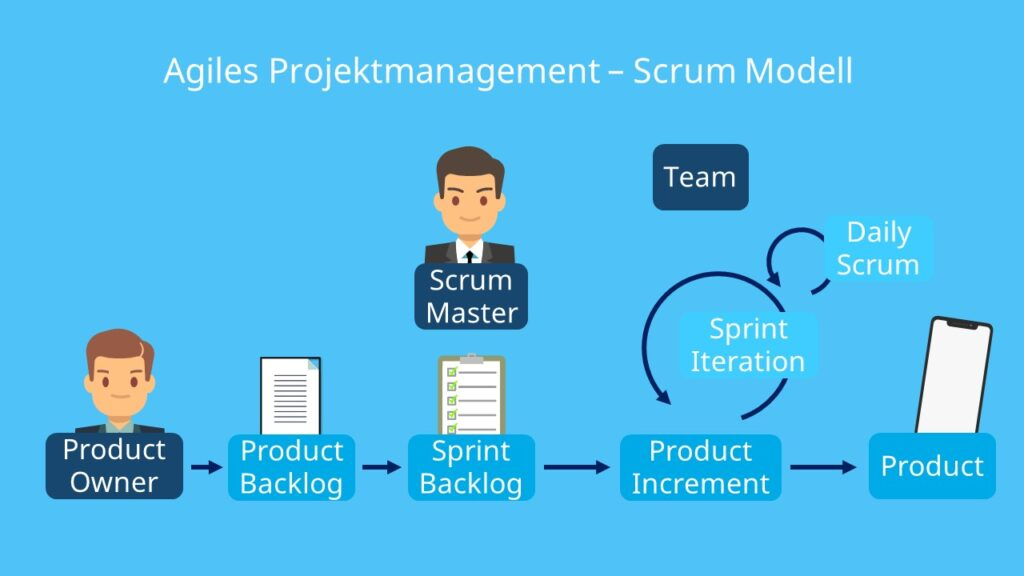
\includegraphics[width=0.9\textwidth]{pics/ScrumAblauf.jpg}
    \centering
    \caption{Veranschaulichung von Scrum https://studyflix.de/wirtschaft/scrum-methode-3426}
    \label{fig:scrum}
\end{figure}

\subsubsection{Product Backlog}
Der Product Backlog enthält sämtliche Anforderungen an das Produkt. Diese Anforderungen werden 
Schritt für Schritt in Sprints bearbeitet. In einem separaten Meeting wird dann entschieden, 
welche Anforderungen aus dem Product Backlog im jeweiligen Sprint abgearbeitet werden. Der Backlog
kann Qualitätsanforderungen, Funktionale Anforderungen, User Stories, Fehler (Bugs) und 
Verbesserungen enthalten. \cite{noauthor_scrum_nodate}

\subsubsection{Burn Down Chart}
Burn Down Charts visualisieren die Arbeit, die zum aktuellen Zeitpunkt noch zu erledigen ist. 
Es lässt sich anhand des Diagrammes die Arbeitsgeschwindigkeit des Teams ableiten.
Das Burn Down Chart eignet sich weiters dafür, die Interaktionen bzw. Sprints zu kontrollieren und 
wenn nötig kontrollierend eingreifen. \cite{noauthor_burn-down-chart_2021}, \cite{noauthor_was_nodate-4}

\subsubsection{GitHub-Tokens}
Persönliche Zugangs-Token (PATs) sind eine Alternative zur Verwendung von Passwörtern für die 
Authentifizierung bei GitHub. Als Sicherheitsvorkehrung entfernt GitHub automatisch persönliche 
Zugangstoken, die seit einem Jahr nicht mehr verwendet wurden. Seit Juli 2020 sind 
Authentifizierungstoken statt Passwörter zu verwenden. \cite{noauthor_token_2020}, \cite{noauthor_creating_nodate}

\section{Problemlösung}
\subsection{GitHub}
Die Wahl Git zur Versionskontrollierung und Kollaboration zu verwenden, ist aus offensichtlichen Gründen der einfachen 
Zusammenarbeit und Codezusammenführung getroffen worden. Für den Provider wurde sich für GitHub entschieden, da das Team 
viel Erfahrung im Umgang mit der Plattform besitzt und daher der Gebrauch naheliegend ist. In Abbildung (siehe Abb. \ref{fig:gituse}) wird die Verwendung 
von GitHub gezeigt. In Abbildung (siehe Abb. \ref{fig:gituse2}) wird die gemeinsame und parallele Arbeit dargestellt. 
Das Zusammenfügen des Quellcodes konnte hauptsächlich durch Git automatisch durchgeführt werden. Einige Zusammenfügungen mussten allerdings 
manuell abgewickelt werden. 

\begin{figure}[H]
    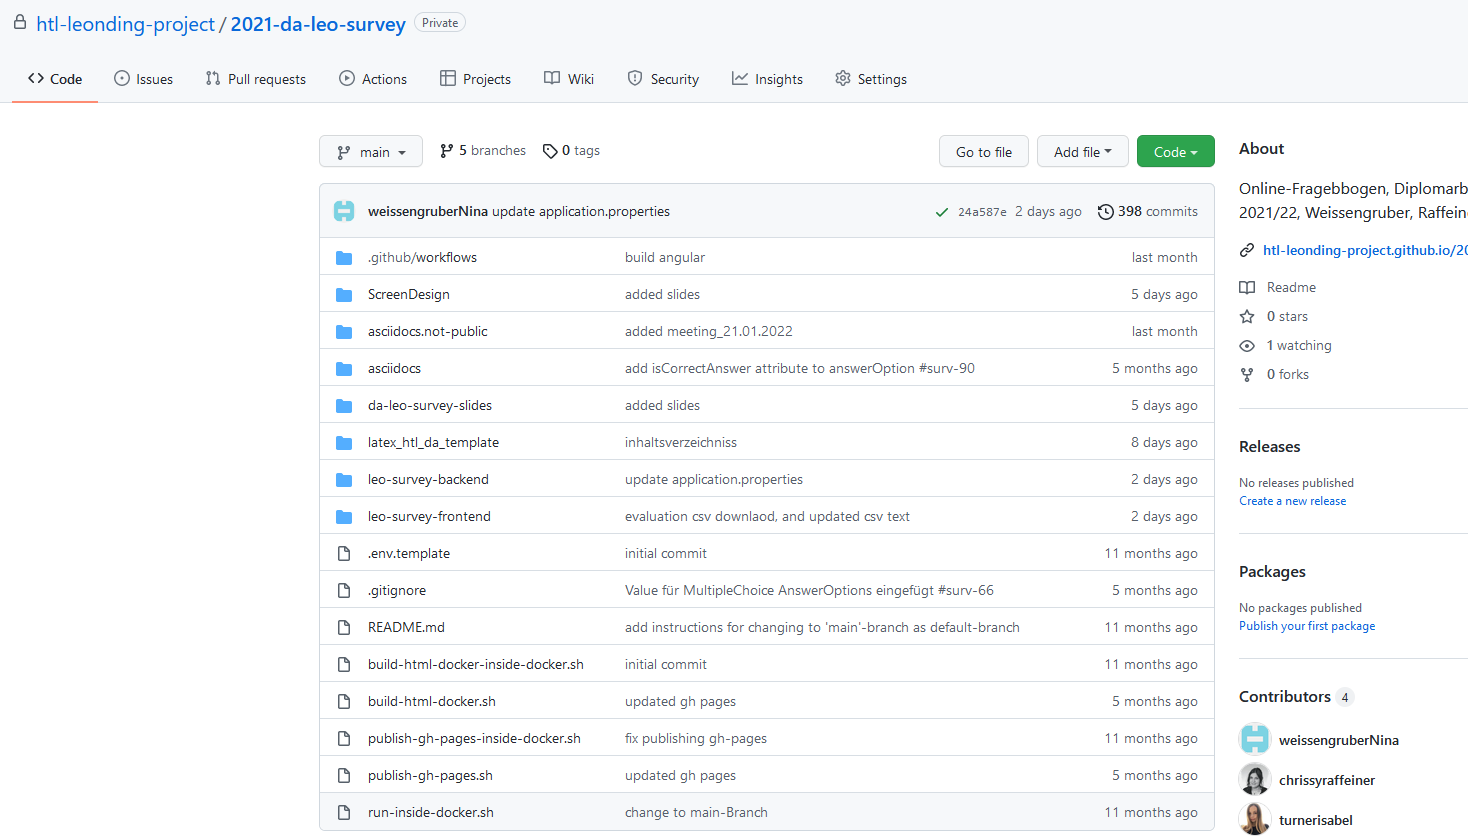
\includegraphics[width=1.0\textwidth]{pics/GitHub.PNG}
    \centering
    \caption{GitHub Repository von Leo-Survey}
    \label{fig:gituse}
\end{figure}

\begin{figure}[H]
    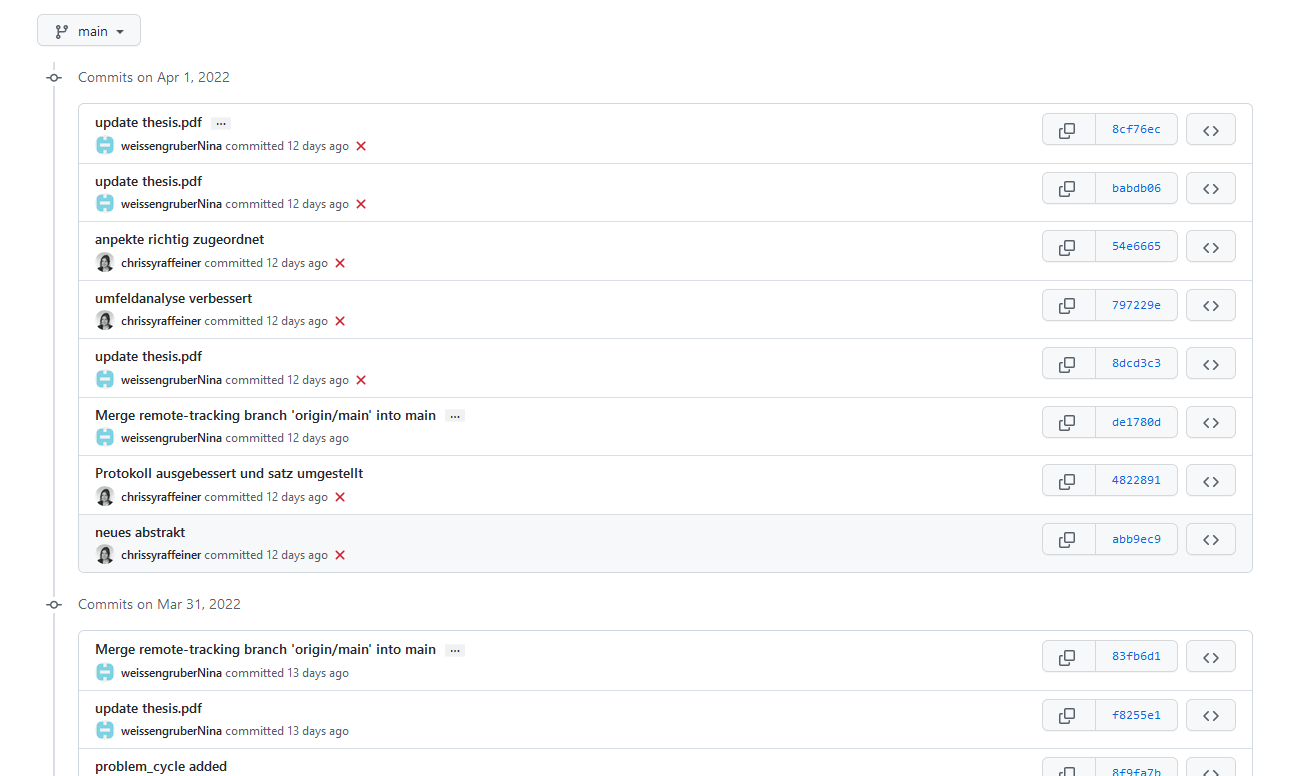
\includegraphics[width=1.0\textwidth]{pics/ComittHistory.PNG}
    \centering
    \caption{GitHub Repository von Leo-Survey Commites}
    \label{fig:gituse2}
\end{figure}

\subsection{GitDesktop}
Die Abbildung (siehe Abb. \ref{fig:git1}) zeigt die Verwendung von GitHub Desktop.
GitHub Desktop wurde hauptsächlich aus dem Grund verwendet, da zwei einzeln geöffnete Anwendungen (IntelliJ für das Backend) 
und (Visual Studio Code für das Frontend) die Änderungen des jeweils 
anderen Programmes nicht erkennen. Durch einen Neustart konnten die Änderungen dann erkannt werden. 
Da dies allerdings mit Aufwand verbunden ist wurde drauf verzichtet und 
GitHub Desktop verwendet. Die Anwendung löste dieses Problem.
\begin{figure}[H]
    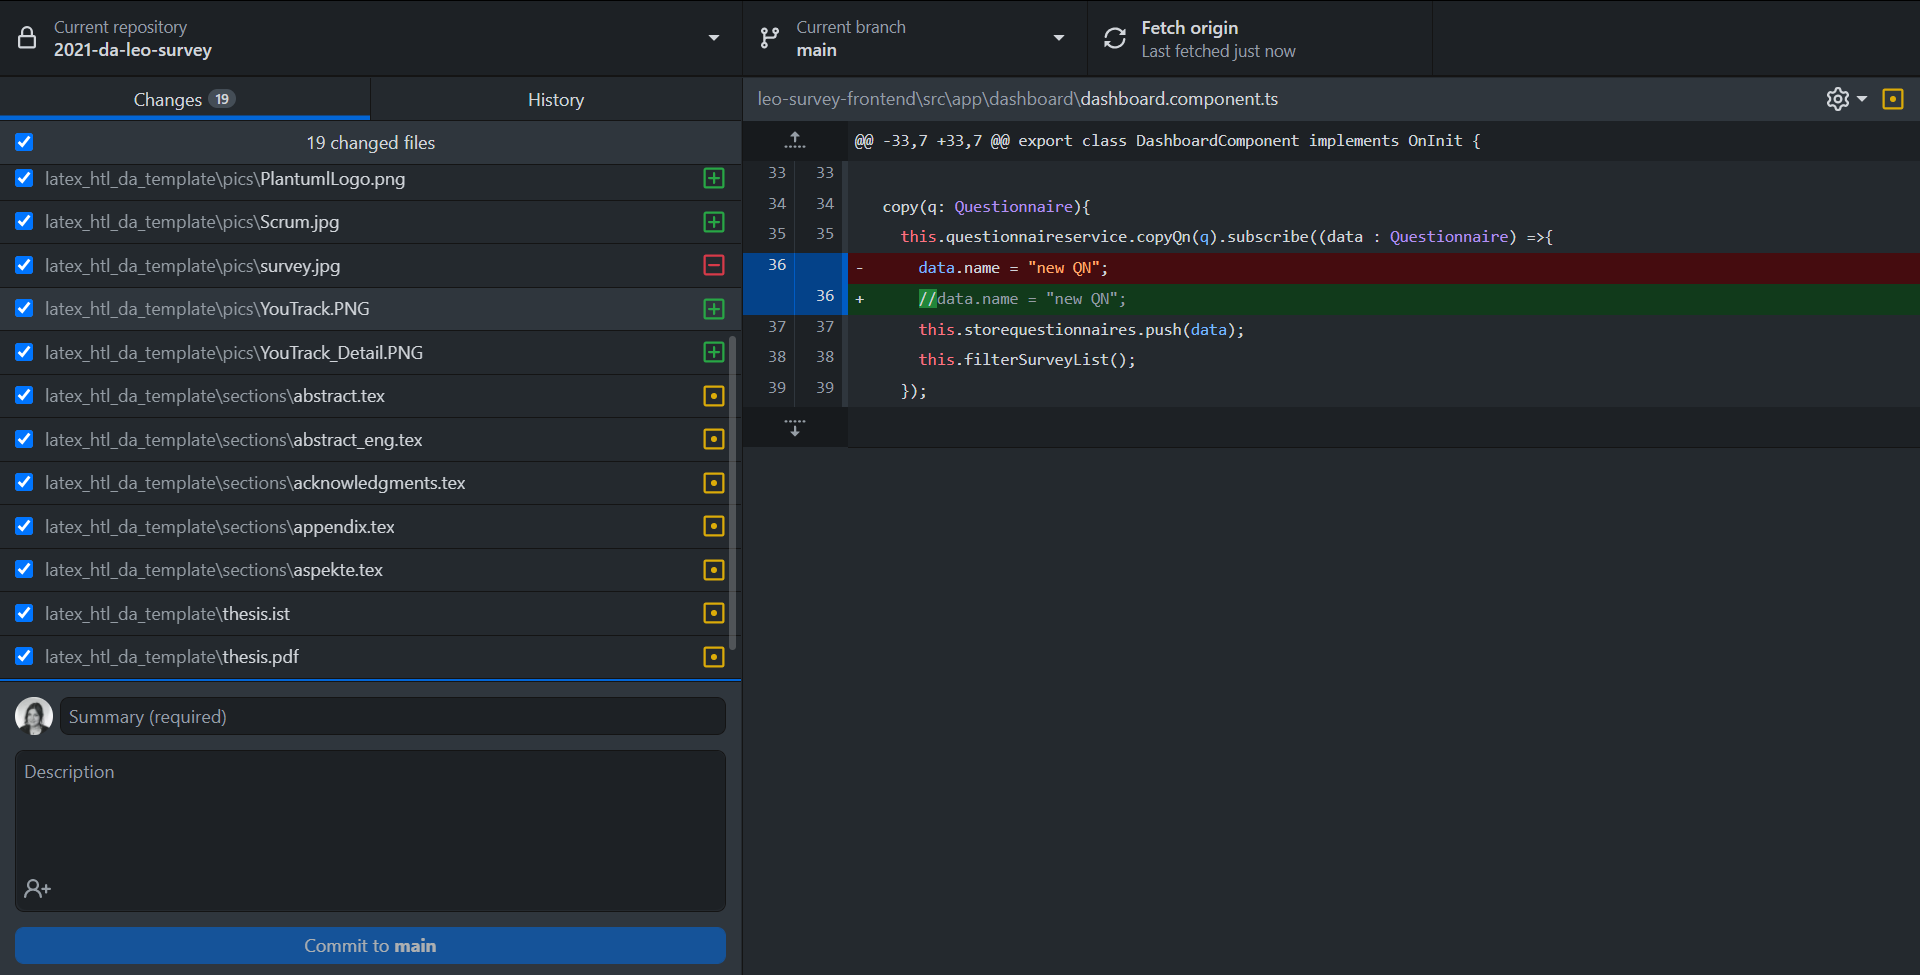
\includegraphics[width=1.0\textwidth]{pics/GitDesktop.PNG}
    \centering
    \caption{GitHub Desktop Beispiel}
    \label{fig:git1}
\end{figure}

\subsection{YouTrack}
Obwohl für das Projekt GitHub verwendet wurde, wurde sich gegen die Verwendung von GitHub Projektboards, Issues und Meilensteine
entschieden und für den Gebrauch von YouTrack. Hauptgrund dafür war, dass im Gegensatz zu GitHub, 
Tasks, Sprints etc. in YouTrack auf einer Seite übersichtlicher dargestellt werden konnten und auch 
zusätzliche Features wie das Burn Down Chart zu Verfügung stehen. Verbindet man YouTrack außerdem 
mit einem GitHub Repository verfügt man über die Funktion von automatisch einzuordnenden
Tasks. Die Projektboards wurden mit der YouTrack-Vorlage Kanban erstellt. 
Diese Vorlage erstellt automatisch 4 Schwimmbahnen (Open, In Progress, To Verify und Done). Die Vorlage kann bearbeitet werden. 
Es wurde allerdings auf eine Änderung verzichtet, da die Vorlage für die vorliegende Arbeit ausgereicht hat.

Die Abbildung (siehe Abb. \ref{fig:youtracksprint}) zeigt beispielhaft einen Sprint der Arbeit.
\subsection{GitHub-Anbindung in YouTrack}
\begin{figure}[H]
    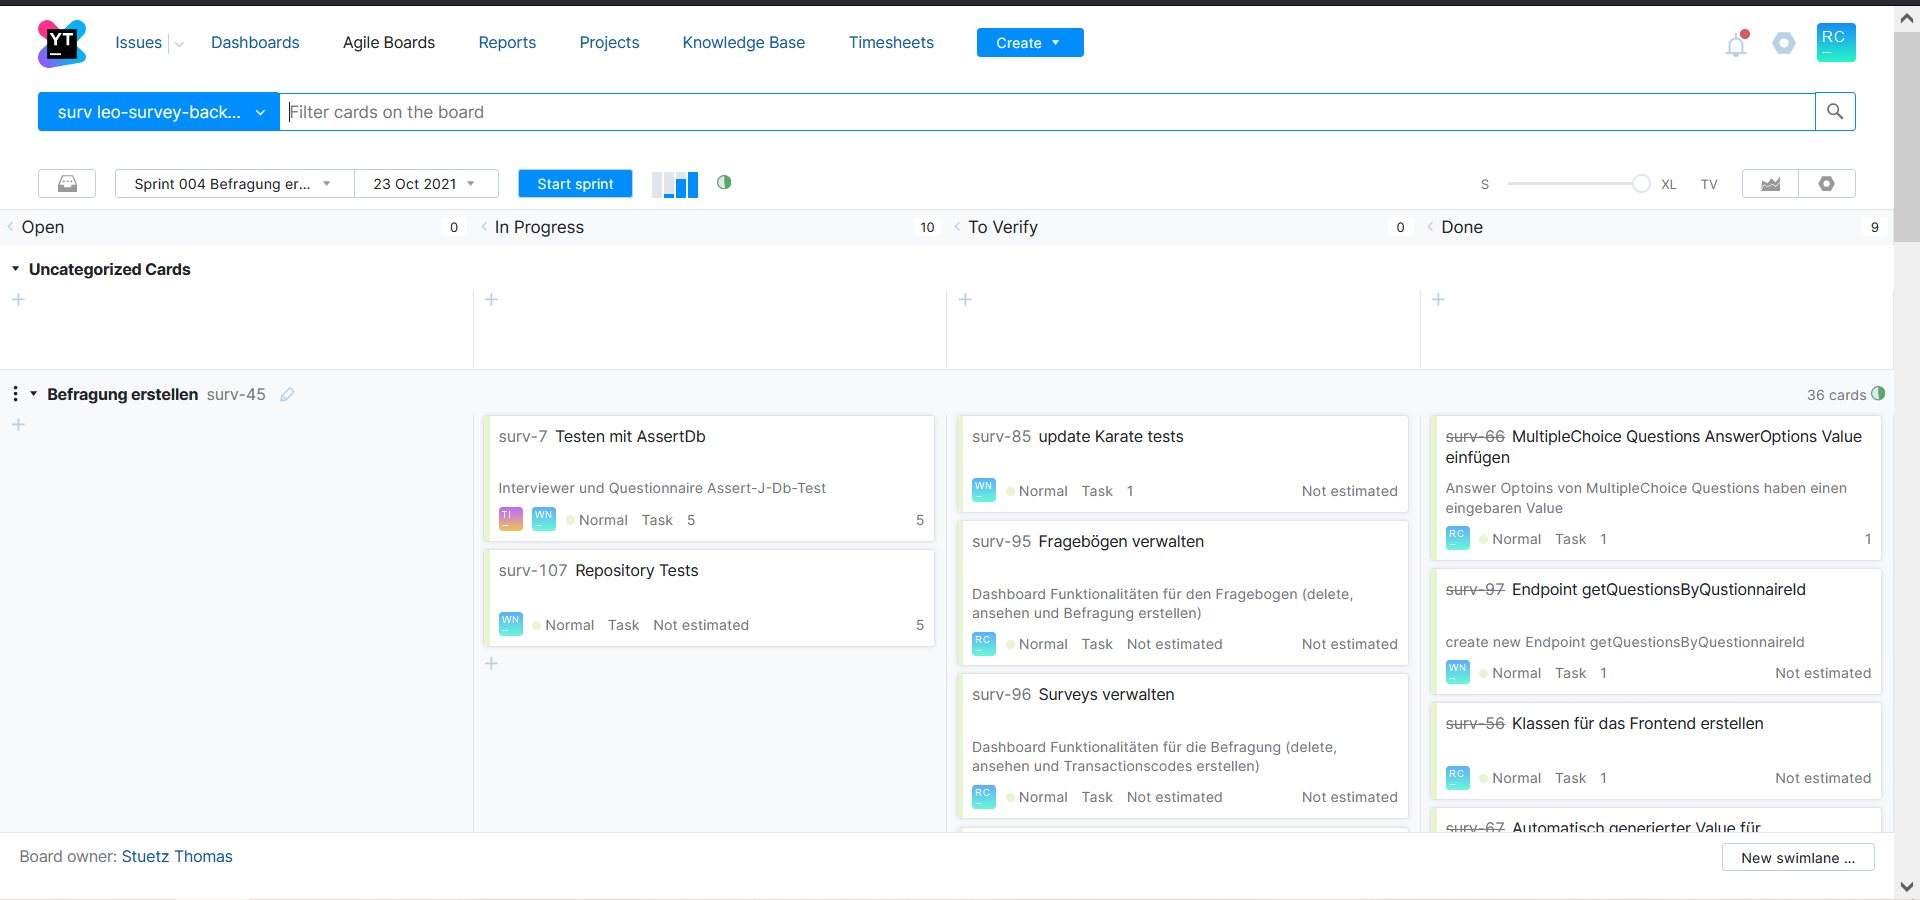
\includegraphics[width=1.0\textwidth]{pics/YouTrack.PNG}
    \centering
    \caption{YouTrack Sprint Beispiel}
    \label{fig:youtracksprint}
\end{figure}

Für designtechnische Aspekte, wie die Erstellung des Logos, Hintergrundbildes und ScreenDesigns wurde ein eigenes Projektboard 
erstellt. (siehe Abb. \ref{fig:youtracksprint2})  
\begin{figure}[H]
    \includegraphics[width=1.0\textwidth]{pics/YouTrackfrontendboard.PNG}
    \centering
    \caption{GitHub-Anbindung in YouTrack}
    \label{fig:youtracksprint2}
\end{figure}

Abbildung (siehe Abb. \ref{fig:burndownchart}) zeigt beispielsweise ein Burn Down Chart aus der vorliegenden Arbeit.
Das Chart zeigt den Arbeitsaufwand des Deployments.  
Die grüne Line gibt den idealen Verlauf des noch zu tätigenden Arbeitsaufwandes an, sodass am Ende des Sprints alle Aufgaben erledigt sind.
Die blaue Line zeigt den tatsächlichen Verlauf des Arbeitsaufwandes und gibt Auskunft darüber, dass bis zum Ende des Sprints noch 
Arbeit zu erledigen ist. Zudem lässt sich daraus schlussfolgern, dass das Team die Vorgaben, bis zu diesem Zeitpunkt, 
eingehalten hat. (blaue Linie verläuft unter der grünen)
\begin{figure}[H]
    \includegraphics[width=1.0\textwidth]{pics/YouTrackBurnDownChart.PNG}
    \centering
    \caption{YouTrack Burn Down Chart Beispiel}
    \label{fig:burndownchart}
\end{figure}

Die Abbildung (siehe Abb. \ref{fig:youtrackGit}) zeigt die Anbindungen von YouTrack an das GitHub Repository, 
die dazu dient, beide Programme miteinander zu vereinen.
Wird ein Task in einer Commit-Message erwähnt, werden diese sonstigen Änderungen in der Detailansicht 
des Tasks angezeigt. Jeder angelegte Task bekommt eine Kennung in der Form \#surv-<zahl> (in diesem Beispiel
\#surv-7) und wird automatisch bei Erwähnung in einer Commit-Nachricht erkannt. Folgt auf die Kennung noch eine 
Bezeichnung einer Schwimmbahn wird der Task automatisiert in die angegebene 
Schwimmbahn geschoben (als Beispiel \#surv-7 To Verify). \cite{noauthor_youtrack_nodate}, \cite{noauthor_agile_nodate}
\begin{figure}[H]
    \includegraphics[width=1.0\textwidth]{pics/YoutrackGitCon.PNG}
    \centering
    \caption{GitHub-Anbindung in YouTrack}
    \label{fig:youtrackGit}
\end{figure}

\begin{spacing}{1}
\chapter{ScreenDesign}\label{chapter:implementation}
\end{spacing}
\section{Handskizzen}
\setauthor{Raffeiner Christine}

Aus den Erkenntnissen der Umfeldanalyse wurden in der ersten Instanz einfache Handskizzen (siehe Abb. \ref{fig:skizzen1} und \ref{fig:skizzen2}) für das Design angefertigt.
Bereits in den ersten Skizzen kristallisierten sich spezielle Ideen, wie zum Beispiel das Dashboard, heraus.

\begin{figure}[H]
    \includegraphics[width=1.0\textwidth]{pics/Handskizze.jpg}
    \centering
    \caption{Skizze Seite 1}
    \label{fig:skizzen1}
\end{figure}

\begin{figure}[H]
    \includegraphics[width=1.0\textwidth]{pics/Handskizze2.jpg}
    \centering
    \caption{Skizze Seite 2}
    \label{fig:skizzen2}
\end{figure}

\newpage

\section{Screendesign Prototyp}
\setauthor{Raffeiner Christine}
Als wichtiger Zwischenschritt zwischen den Skizzen und dem Prototypen wurde ein Moodboard erstellt, dass die grundlegende 
Stimmung der Webseite, wichtige Elemente der zukünftigen Webseite, Schriften und Farben darstellt. Im Moodboard (siehe Abb. \ref{fig:moodboard}) 
wurden die wichtigsten Elemente für die stufenweise Erstellung des Fragebogens, die Fortschrittsanzeige für die 
Beantwortung einer Umfrage und die wichtigsten Funktionen des Dashboard (durch die Icons symbolisiert) erstmals dargestellt.

\begin{figure}[H]
    \includegraphics[width=0.8\textwidth]{pics/Moodboard.png}
    \centering
    \caption{Moodboard Leo-Survey}
    \label{fig:moodboard}
\end{figure}

Nach der Erstellung des Moodboards wurden die Skizzen im Programm Adobe XD umgesetzt. 
Es wurde auf das zukünftige Design mit 
Angular Materials Rücksicht genommen und die Elemente möglichst in dem Design von Materials erstellt.

\begin{figure}[H]
    \includegraphics[width=0.8\textwidth]{pics/Startseite.png}
    \centering
    \caption{ScreenDesign Startseite}
    \label{fig:screenDesign2}
\end{figure}

\begin{figure}[H]
    \includegraphics[width=0.8\textwidth]{pics/Login.png}
    \centering
    \caption{ScreenDesign Login}
    \label{fig:screenDesign1}
\end{figure}
    
\begin{figure}[H]
    \includegraphics[width=0.8\textwidth]{pics/Dashboard.png}
    \centering
    \caption{ScreenDesign Dashboard}
\end{figure}

\begin{figure}[H]
    \includegraphics[width=0.8\textwidth]{pics/Erstellen_Umfarage_1.png}
    \centering
    \caption{ScreenDesign Fragebogen erstellen}
\end{figure}

\begin{figure}[H]
    \includegraphics[width=0.8\textwidth]{pics/Erstellen_Umfarage_2.png}
    \centering
    \caption{ScreenDesign Fragebogen erstellen}
\end{figure}

\begin{figure}[H]
    \includegraphics[width=0.4\textwidth]{pics/Erstellen_Umfarage_2_1.png}
    \centering
    \caption{ScreenDesign Fragebogen erstellen}
\end{figure}

\begin{figure}[H]
    \includegraphics[width=0.4\textwidth]{pics/Erstellen_Umfarage_2_2.png}
    \centering
    \caption{ScreenDesign Fragebogen erstellen}
\end{figure}

\begin{figure}[H]
    \includegraphics[width=0.8\textwidth]{pics/Erstellen_Umfarage_3.png}
    \centering
    \caption{ScreenDesign Fragebogen erstellen}
\end{figure}

\begin{figure}[H]
    \includegraphics[width=0.8\textwidth]{pics/Erstellen_Umfarage_4.png}
    \centering
    \caption{ScreenDesign Fragebogen erstellen}
\end{figure}

\begin{figure}[H]
    \includegraphics[width=0.8\textwidth]{pics/Fargebogen ausfuellen.png}
    \centering
    \caption{ScreenDesign Fragebogen ausfüllen}
\end{figure}

Die Login-Seite (siehe Abb. \ref{fig:screenDesign1}) wurde im Produktivsystem mit der des Keycloaks ersetzt. Auch andere kleinere Elemente wie der 
Footer auf der Startseite (siehe Abb. \ref{fig:screenDesign2}) wurden in der Engversion abgeändert. Die Endversion befindet sich in Kapitel 
\ref{chapter:ergebnis} auf S. \pageref{chapter:ergebnis}.

\begin{spacing}{1}
\chapter{Ergebnis}
\label{chapter:ergebnis}
\end{spacing}
\setauthor{Raffeiner Christine}
\section{Zusammenfassung}
Ergebnis der Arbeit ist eine lauffähige Applikation bestehend aus Frontend, Backend, Keycloak und Datenbank.
Alle Komponenten wurden gelockert und auf eine VM deployed. Für die Sicherheit sorgt eine Sperre der Ports für die VM und der 
Reverse-Proxy Traefik.

\section{Frontend}
Es folgen Abbildung der wichtigsten Unterseiten und Funktionalitäten der Arbeit. \cite{noauthor_felx-box_nodate}, \cite{noauthor_w3schools_nodate}, \cite{noauthor_wait_nodate}
\begin{figure}[H]
    \includegraphics[width=0.9\textwidth]{pics/Ergebnis_Startseite.PNG}
    \centering
    \caption{Startseite}
\end{figure}

\begin{figure}[H]
    \includegraphics[width=0.9\textwidth]{pics/Ergebniss_KC.PNG}
    \centering
    \caption{Login mittels Keycloak}
\end{figure}
Mithilfe des Keycloak können sich die Schüler/innen und Lehrer/innen mit dem gewohnten Anmeldedaten anmelden.   

\begin{figure}[H]
    \includegraphics[width=0.9\textwidth]{pics/Ergebnis_Dashboard.PNG}
    \centering
    \caption{Dashboard}
\end{figure}

Auf dem Dashboard werden alle für den / die Benutzer/in verfügbaren Fragebögen und Umfragen angezeigt.
Alle Fragebögen und Umfragen, die im Besitz einer Person sind, können geändert und gelöscht werden. Von anderen Fragebögen können 
Kopien erstellt werden. Fragebögen können gefiltert werden. Umfragen können erstellt und ausgewertet werden.

\begin{figure}[H]
    \includegraphics[width=0.9\textwidth]{pics/Ergebnis_Erstellen.PNG}
    \centering
    \caption{Fragebogen erstellen}
\end{figure}

\begin{figure}[H]
    \includegraphics[width=0.9\textwidth]{pics/Ergebnis_Erstellen2.PNG}
    \centering
    \caption{Startseite}
\end{figure}

Fragebögen können stufenweise erstellt werden. Es kann zwischen vier verschieden Fragetypen gewählt werden.

\begin{figure}[H]
    \includegraphics[width=0.9\textwidth]{pics/Ergebnis_Antworten.PNG}
    \centering
    \caption{Startseite}
\end{figure}

Das Beantworten der Umfrage erfordert keinen Login und wird mithilfe von Transaktionscodes durchgeführt. 
Fragen werden in kleinen Gruppen zusammengefasst, angezeigt und können optional beantwortet werden. 
Vor dem Abschicken wird dem/er Benutzer/in angezeigt, wie viele Fragen er / sie nicht beantwortet hat.
	
\begin{spacing}{1}
\chapter{Resümee}
\label{chapter:resumme}
\end{spacing}
\setauthor{Weissengruber Nina}
\subsection{Meilensteine}
Für eine Evaluation der Meilensteine siehe Kapitel Meilensten Analyse \ref{meilensteile}.
\subsection{Kommunikation}

Kommunikation ist ein wichtiger Punkt bei Projektarbeiten. Deshalb wurde auch bei dieser Arbeit großer 
Wert auf eine bestmögliche Kommunikation gelegt. 
\newline
\newline
Die Kommunikation im Team ist von beiden Parteien als angenehm empfunden worden.
Man konnte sich immer auf seinen Teampartner verlassen und konnte damit rechnen, dass Aufgaben und Fehler 
schnellstmöglich erledigt, beziehungsweise behoben werden. Bei auftretenden Problemen wurde Kritik immer
objektiv formuliert und angenommen. 
Bei der Vereinbarung von Meetings konnte sich das Team immer rasch auf ein Datum und Uhrzeit einigen.
Auch mit dem Betreuer konnte sich schnell auf einen Zeitpunkt geeinigt werden.
Die Projektkommunikation im Entwicklerteam intern hat primär auf YouTrack stattgefunden, aber auch
persönliche Gespräche waren ein wichtiger Bestandteil. Die wichtigsten Informationen für den Betreuer
wurden per E-Mail übermittelt, aber auch hier wurde großer Wert auf das persönliche Gespräch gelegt.

\subsection{Probleme während der Implementierung}
Wir hatten große Schwierigkeiten bei der Einhaltung des Zeitplans, da wir den Umfang des Projektes falsch eingeschätzt haben.
Außerdem hatten wir Probleme bei den Technologien, bei deren Umsetzung manche Aspekte davon neu erlernt werden mussten.


\appendix
\addchap{Anhang}
\chapter{Teamvorstellung}
\setauthor{Raffeiner Christine, Weissengruber Nina}
\subsection{Team}
\subsubsection{Raffeiner Christine}
\begin{wrapfigure}{r}{0.3\textwidth}
    \begin{center}
      \includegraphics[width=0.3\textwidth]{pics/Chrissy.jpg}
    \end{center}
\end{wrapfigure}
Christine Raffeiner ist eine 20 Jahre junge Musterschülerin, die viel Zeit und Mühe investiert um ihre 
schulischen Ziele zu erreichen. Sie ist bereits das sechste Jahr an der HTL Leonding, jedoch ist sie in 
allen Fächern eine der Besten aus ihrer Klasse und ist auch gerne bereit anderen zu helfen und ihnen 
Fragen zu erklären. Zusätzlich zu ihrer Hilfsbereitschaft strahlt sie Fröhlichkeit aus und ist eine Person 
mit der man gern über alle möglichen Themen spricht, egal ob schulischer oder privater Natur.
\newline
\subsubsection{Weissengruber Nina}
\begin{wrapfigure}{r}{0.3\textwidth}
    \begin{center}
      \includegraphics[width=0.3\textwidth]{pics/nina.jpg}
    \end{center}
\end{wrapfigure}
Nina Weissengruber die perfekte Ergänzung für jedes Team und ein richtiges Energiepacket, die die 
Aufmerksamkeit auf sich zieht.  
Nina ist eine hervorragende Schülerin, die man sich zum 
Vorbild nehmen kann und muss, denn sie schafft es ohne große Hindernisse, zu bestehen. Besonders erwähnenswert sind auch 
ihre ausgezeichneten Kenntnisse in Mathematik und Apex.

\subsubsection{Über Uns}
Zusammenfassend ist noch zu sagen, dass wir ausgezeichnet zusammenarbeiten konnten, obwohl wir uns vor unserem Projekt  nicht wirklich gut kannten. 
Unsere Arbeitsweise betrachtend spielten wir gut zusammen 
und verfolgten ohne viel Absprache die selben Ziele.

\chapter{Wichtige Lektionen}
\setauthor{Raffeiner Christine, Weissengruber Nina}
Die offensichtlichste Lektion die wir gelernt haben, war die Handhabung von längerfristigen Projekten, die 
hohe Priorität und gewisse Eigenverantwortung mit sich ziehen. Um das noch weiter zu führen wurden auch die 
Erfahrungen gemacht, die Projektarbeit völlig außerhalb der Schulstunden neben Schul- und Lernstress mit sich 
bringen. Dazu zählen besonders das Einteilen von Aufgaben und Zeitmanagement. Persönliche Erfahrungen wurden 
besonders im Bereich der Testimplementierung und Wichtigkeit dieser erzielt. Auch wurde außerhalb der 
bereits erlernten Kenntnisse wissen im Bereich des Keycloak und Reverse-Proxy gesammelt. Rückschließend sind 
wir zu dem Entschluss gekommen, dass die stressfreie Zeit während der Sommerferien besser hätten nutzen sollen.

\chapter{Protokolle}
\setauthor{Raffeiner Christine}
Folgend befinden sich sämtliche Gesprächsprotokolle der Meetings, die das Team im Laufe 
der Arbeit mit ihrem Betreuer Herrn Professor Thomas Stütz geführt hat. 
\newline
Die Protokolle stellen eine Zusammenfassung der jeweiligen Meetings dar. \cite{noauthor_asciidock_nodate}

\includepdf{./protocols/meeting_29.04.2021}

\includepdf{./protocols/meeting_01.07.2021}

\includepdf{./protocols/meeting_15.07.2021}

\includepdf{./protocols/meeting_16.07.2021}
\includepdf[page=2]{./protocols/meeting_16.07.2021}

\includepdf{./protocols/meeting_05.08.2021}

\includepdf{./protocols/meeting_09.08.2021}

\includepdf{./protocols/meeting_10.08.2021}

\includepdf{./protocols/meeting_24.08.2021}

\includepdf{./protocols/meeting_31.08.2021}

\includepdf{./protocols/meeting_07.10.2021}

\includepdf{./protocols/meeting_22.10.2021}

\includepdf{./protocols/meeting_21.01.2022}
\includepdf[page=2]{./protocols/meeting_21.01.2022}

\chapter{Meilensteinliste und -analyse}
\label{meilensteile}
\setauthor{Raffeiner Christine}
Die erste Version der Meilensteinliste sah vor, dass die Arbeit innerhalb des Sommers,
während der Sommerferien implementiert und bis zu Schulbeginn fertiggestellt wird. 
\begin{table}[H]
    \centering
    \caption{Meilensteinliste Version 1}
    \label{tab:meilensteine1}
    \begin{tabular}{|c|l|}
        \hline
        05.07.2021 & Datenmodell fertiggestellt \\ \hline
        19.07.2021 & Backend (mit Endpoints) zum Ausfüllen eines vorhandenen Fragebogens erstellt \\ \hline
        02.08.2021 & Frontend zum Ausfüllen eines vorhandenen Fragebogens erstellt \\ \hline
        09.08.2021 & Backend (mit Endpoints) zum Erstellen eines Fragebogens erstellt \\ \hline
        23.08.2021 & Frontend zum Ausfüllen von Fragebögen erstellt \\ \hline
        13.09.2021 & Gesamtsystem mit Benutzerverwaltung und Docker-Deployment fertiggestellt \\ \hline
        \end{tabular}
\end{table}

Im Laufe des Sommers stellte sich bald heraus, dass diese Meilensteine aus vielerlei Gründen 
nicht eingehalten werden konnten. 
Die Meilensteine, (siehe Tabelle \ref{tab:meilensteine1}) (1) Datenmodell fertiggestellt und (2) Backend (mit Endpoints) 
die zum Ausfüllen eines vorhandenen Fragebogens erstellt, 
wurden in den Ferien verspätet fertiggestellt. Daraus folgend hat das Team die Meilensteine angepasst und eine neue
Liste erstellt (siehe Tabelle \ref{tab:meilensteine2}).

\begin{table}[H]
    \centering
    \caption{Meilensteinliste Version 2}
    \label{tab:meilensteine2}
    \begin{tabular}{|l|l|}
        \hline
        05.11.2021 & Backend und Frontend Funktionen zum Fragebogen erstellen fertiggestellt \\ \hline
        10.11.2021 & Frontend Dashboard fertiggestellt \\ \hline
        19.11.2021 & Backend und Frontend Funktionen zum Fragebogen ausfüllen fertiggestellt \\ \hline
        29.11.2021 & Backend zum Fragebogen ausfüllen fertiggestellt \\ \hline
        20.12.2021 & Backend und Frontend Login mittels Keycloak fertiggestellt \\ \hline
        10.01.2022 & Gesamtsystem Docker-Deployment fertiggestellt \\ \hline
    \end{tabular}
\end{table}

Die neue Meilensteinliste verschob die noch nicht erledigten Meilensteine nach hinten - mit dem Datum der 
Erreichung des letzten Meilensteines in den Winterferien. Das Team konnte auch  
diese Meilensteine nicht eingehalten. Da nun die Fertigstellung der Implementierung im Vordergrund 
stand wurden keine neuen Meilensteine mehr definiert und es wurde ohne Meilensteinliste auf die Fertigstellung hingearbeitet.
\newline
\newline
Schlussfolgernd ist zu sagen, dass die ursprünglichen Meilensteine oder zumindest die 2. Version der Liste, eingehalten hätten werden sollen.
Das Team ließ sich viel zu viel Zeit und war auch wenig konsequent mit der Einhaltung der gesetzten Ziele.
Zusätzlich wurde der gesamte Arbeitsumfang der Arbeit stark unterschätzt.

\chapter{Arbeitsverteilung}
\setauthor{Raffeiner Christine, Weissengruber Nina}
Die Arbeitsaufteilung war von Anfang an schnell und ohne Probleme entschieden. 
Die Programmierung des Backend und Testung fiel dabei Nina zu und Implementierung und Erstellung des Designs 
des Frontend wurde Christine überlassen. Außerdem wurde entschieden, dass Nina das Deployment übernimmt und 
Christine den Keycloak implementiert.

\subsection{Schriftliche Arbeitsteilung}
\begin{compactenum}
    \item Danksagung, Zusammenfassung und Inhaltsverzeichnis \big [ R \big ]
    \item Einleitung \big [ R \& W \big ]
    \item Ausgangssituation \big [ W \big ]
    \item Umfeldanalyse \big [ R \big ]
    \begin{compactenum}
        \item Vorgänger Projekte \big [ R \big ]
        \item Online Fragebogenwerkzeuge \big [ R \big ]
    \end{compactenum}
    \item Problembeschreibung \big [ W \big ]
    \item Aufgabenstellung \big [ W \big ]
    \item Ziele \big [ R \& W \big ]
    \item Systemarchitektur \big [ R \& W \big ]
    \item \begin{compactenum}
        \item Aktivitätsdiagramm \big [ W \big ]
        \item Klassendiagramm und Entity-Relationship-Modell \big [ R \big ]
    \end{compactenum}
    \item Technologien \big [ R \& W \big ]
    \begin{compactenum}
        \item Angular \big [ R \big ]
        \item Docker \big [ R \big ]
        \item Keycloak \big [ R \big ]
        \item Traefik \big [ R \big ]
        \item Oracle SQL-Developer \big [ R \big ]
        \item PlantUML \big [ R \big ]
        \item Markdown \big [ R \big ]
        \item Java \big [ W \big ]
        \item Quarkus \big [ W \big ]
        \item PostgreSql \big [ W \big ]
        \item Rest-API \big [ W \big ]
        \item Software Testing \big [ W \big ]
    \end{compactenum}
    \item Ausgewählte Aspekte \big [ R \& W \big ]
    \begin{compactenum}
        \item Besonders gut gelöste Programmteile \big [ R \& W \big ]
        \item Besondere Probleme die gelöst wurden \big [ R \& W \big ]
        \item Entwurfsentscheidung \big [ R \& W \big ]
    \end{compactenum}
    \item Implementierung \big [ W \big ]
    \item Projektorganisation \big [ R \big ]
    \begin{compactenum}
        \item Anforderungen \big [ R \big ]
        \item Mögliche Hilfsmittel \big [ R \big ]
        \item Problemlösung \big [ R \big ]
    \end{compactenum}
    \item ScreenDesign \big [ R \big ]
    \item \begin{compactenum}
        \item Handskizzen \big [ R \big ]
        \item ScreenDesign Prototyp \big [ R \big ]
    \end{compactenum}
    \item Ergebnis \big [ R \big ]
    \item \begin{compactenum}
        \item Zusammenfassung \big [ R \big ]
        \item Frontend \big [ R \big ]
    \end{compactenum}
    \item Resümee \big [ R \& W \big ]
    \item Anhang \big [ R \& W \big ]
    \begin{compactenum}
        \item Teamvorstellung \big [ R \& W \big ]
        \item Wichte Lektionen \big [ R \& W \big ]
        \item Protokolle \big [ R \big ]
        \item Meilensteinliste und -analyse \big [ R \big ]
        \item Arbeitsteilung \big [ R \& W \big ]
    \end{compactenum}
\end{compactenum}

\newpage
\spacing{1}{
%\bibliographystyle{IEEEtran}
\bibliographystyle{ieeetrande}
\bibliography{bib}
}


% Usage:
% \gls{label} lowercase in text
% \Gls{label} Uppercase in text
% \newacronym{label}{abbrev}{full}
% \newglossaryentry{label}{settings}
\printglossary[title=Glossar,toctitle=Glossar] %,style=long]
\listoffigures
\listoftables
\lstlistoflistings
	
\end{document}